%%%%%%%%%%%%%%%%%%%%%%%%%%%%%%%%%%%%%%%%%%%%%%%%%%%%%%%%%%
%
% Vzor pro sazbu kvalifikační práce
%
% Západočeská univerzita v Plzni
% Fakulta aplikovaných věd
% Katedra informatiky a výpočetní techniky
%
% Petr Lobaz, lobaz@kiv.zcu.cz, 2016/03/14
%
%%%%%%%%%%%%%%%%%%%%%%%%%%%%%%%%%%%%%%%%%%%%%%%%%%%%%%%%%%

% Možné jazyky práce: czech, english
% Možné typy práce: BP (bakalářská), DP (diplomová)
\documentclass[czech,DP]{thesiskiv}

% Definujte údaje pro vstupní strany
%
% Jméno a příjmení; kvůli textu prohlášení určete, 
% zda jde o mužské, nebo ženské jméno.
\author{Bc. Ondřej Váně}
\declarationmale

%alternativa: 
%\declarationfemale

% Název práce
\title{Analýza přítomnosti anti-vzorů v datech nástrojů pro řízení projektů}

% 
% Texty abstraktů (anglicky, česky)
%
\abstracttexten{TODO Lorem ksjdfkjdfipsum dolor sit amet, consectetuer adipiscing elit. Curabitur bibendum justo non orci. Etiam quis quam. Proin mattis lacinia justo. In dapibus augue non sapien. Nunc tincidunt ante vitae massa. In rutrum. Fusce consectetuer risus a nunc. Nulla non arcu lacinia neque faucibus fringilla. Praesent dapibus. In laoreet, magna id viverra tincidunt, sem odio bibendum justo, vel imperdiet sapien wisi sed libero. Pellentesque pretium lectus id turpis. Aliquam in lorem sit amet leo accumsan lacinia. Ut enim ad minim veniam, quis nostrud exercitation ullamco laboris nisi ut aliquip ex ea commodo consequat. Integer imperdiet lectus quis justo. Duis condimentum augue id magna semper rutrum.}

\abstracttextcz{TODO Lorem ipsum dolor sit amet, consectetuer adipiscing elit. Curabitur bibendum justo non orci. Etiam quis quam. Proin mattis lacinia justo. In dapibus augue non sapien. Nunc tincidunt ante vitae massa. In rutrum. Fusce consectetuer risus a nunc. Nulla non arcu lacinia neque faucibus fringilla. Praesent dapibus. In laoreet, magna id viverra tincidunt, sem odio bibendum justo, vel imperdiet sapien wisi sed libero. Pellentesque pretium lectus id turpis. Aliquam in lorem sit amet leo accumsan lacinia. Ut enim ad minim veniam, quis nostrud exercitation ullamco laboris nisi ut aliquip ex ea commodo consequat. Integer imperdiet lectus quis justo. Duis condimentum augue id magna semper rutrum.}

% Na titulní stranu a do textu prohlášení se automaticky vkládá 
% aktuální rok, resp. datum. Můžete je změnit:
%\titlepageyear{2016}
%\declarationdate{1. března 2016}

% Ve zvláštních případech je možné ovlivnit i ostatní texty:
%
%\university{Západočeská univerzita v Plzni}
%\faculty{Fakulta aplikovaných věd}
%\department{Katedra informatiky a výpočetní techniky}
%\subject{Bakalářská práce}
%\titlepagetown{Plzeň}
%\declarationtown{Plzni}

%%%%%%%%%%%%%%%%%%%%%%%%%%%%%%%%%%%%%%%%%%%%%%%%%%%%%%%%%%
%
% DODATEČNÉ BALÍČKY PRO SAZBU
% Jejich užívání či neužívání záleží na libovůli autora 
% práce
%
%%%%%%%%%%%%%%%%%%%%%%%%%%%%%%%%%%%%%%%%%%%%%%%%%%%%%%%%%%

% Zařadit literaturu do obsahu
\usepackage[nottoc,notlot,notlof]{tocbibind}

% Umožňuje vkládání obrázků
\usepackage[pdftex]{graphicx}
\usepackage{placeins}
\usepackage{float}
\usepackage{pdflscape}
\floatstyle{plaintop}
\restylefloat{table}

% Přidání znaku checkmark a cross
\usepackage{amssymb}% http://ctan.org/pkg/amssymb
\usepackage{pifont}% http://ctan.org/pkg/pifont
\newcommand{\cmark}{\ding{51}}%
\newcommand{\xmark}{\ding{55}}%


% Odkazy v PDF jsou aktivní; navíc se automaticky vkládá
% balíček 'url', který umožňuje např. dělení slov
% uvnitř URL
\usepackage[pdftex]{hyperref}
\hypersetup{colorlinks=true,
  unicode=true,
  linkcolor=black,
  citecolor=black,
  urlcolor=black,
  bookmarksopen=true}

% Při používání citačního stylu csplainnatkiv
% (odvozen z csplainnat, http://repo.or.cz/w/csplainnat.git)
% lze snadno modifikovat vzhled citací v textu
\usepackage[numbers,sort&compress]{natbib}
\usepackage{listings}
\usepackage{xcolor}

% Definice kódového segmentu 
\definecolor{codegreen}{rgb}{0,0.6,0}
\definecolor{codegray}{rgb}{0.5,0.5,0.5}
\definecolor{codepurple}{rgb}{0.58,0,0.82}
\definecolor{backcolour}{rgb}{0.95,0.95,0.92}

\lstdefinestyle{mystyle}{
    backgroundcolor=\color{backcolour},   
    commentstyle=\color{codegreen},
    keywordstyle=\color{magenta},
    numberstyle=\tiny\color{codegray},
    stringstyle=\color{codepurple},
    basicstyle=\ttfamily\footnotesize,
    breakatwhitespace=false,         
    breaklines=true,                 
    captionpos=b,                    
    keepspaces=true,                 
    numbers=left,                    
    numbersep=5pt,                  
    showspaces=false,                
    showstringspaces=false,
    showtabs=false,                  
    tabsize=2
}

\lstset{style=mystyle}

%%%%%%%%%%%%%%%%%%%%%%%%%%%%%%%%%%%%%%%%%%%%%%%%%%%%%%%%%%
%
% VLASTNÍ TEXT PRÁCE
%
%%%%%%%%%%%%%%%%%%%%%%%%%%%%%%%%%%%%%%%%%%%%%%%%%%%%%%%%%%
\begin{document}
%
\maketitle
\tableofcontents
\chapter{Úvod}
TODO

\chapter{Proces vývoje software}
Vývoj softwaru v dnešní době představuje soubor mnoha různých činností, které napomáhají k úspěšnému dokončení projektu, a tím i uspokojení zákazníka. Mezi tyto aktivity již zdaleka nepatří pouze psaní programového kódu, ale patří sem také například sběr požadavků, kapacitní plánování, návrh architektury, návrh nasazení, testování atd. Všechny tyto činnosti můžeme jednotně nazvat proces vývoje softwaru.
\par
V této kapitole jsou představeny základní pojmy týkající se procesu vývoje softwaru a  jednotlivé metodiky, které se v dnešní době nejčastěji využívají k řízení vývoje softwaru.
\section{Proces}
Proces jsou jednotlivé činnosti, které na sebe navazují a mají určitou posloupnost. Při jednotlivých činnostech dochází k přeměně vstupů na požadované výstupy. Proces se často opakuje a snažíme se ho stále zdokonalovat a optimalizovat.
\par
Proces může být lineární nebo komplikovanější. O lineární proces se jedná, pokud za každou ukončenou činností následuje pouze jedna další činnost nebo konec procesu, tedy výsledek. Oproti lineárnímu procesu může být proces složitější, kde po jedné ukončené činnosti může navazovat několik dalších činností. Dojde tak k větvení procesu, který může být prováděn paralelně několika pracovníky. Následně se opět sbíhá do jednoho výsledku.\cite{ProjektVsProces}
\section{Projekt}
Projekt je jednorázová záležitost, která slouží k vytvoření čí změně něčeho jedinečného, např. vytvoření softwaru, implementace nového informačního systému, uvedení nového výrobku na trh a podobně. Průběh každého projektu bývá unikátní a dopředu ho nelze dokonale popsat a naplánovat. V projektu lze definovat tzv. fáze, které obsahují základní popis, co by se mělo v dané fázi odehrát. Konkrétní činnosti v každé fázi se však mohou v průběhu projektu měnit z důvodu nepředvídatelnosti.
\par
Z tohoto důvodu zavádíme pojem tzv. projektové řízení. Jedná se o činnosti související s plánováním a kontinuálním řízením, jak jednotlivých činností projektu, tak řízení celého projektu. Nejčastěji se projektové řízení využívá při dodávání unikátního softwaru zákazníkům např. implementace informačního systému, vývoj nové podnikové aplikace, konfigurace stávajícího systému dle požadavků zákazníka apod.\cite{ProcesniAProjektoveRizeni}
\section{Prvky softwarového procesu}
V procesu vývoje softwaru se vyskytují čtyři základní prvky, které jsou:
\begin{itemize}
    \item aktivita,
    \item fáze,
    \item artefakt,
    \item role.
\end{itemize}
Celý projekt se rozpadá na jednotlivé činnosti tzv. aktivity. Tyto aktivity můžeme rozdělit do dvou základních skupin. Aktivity technické a podpůrné. Technické aktivity jsou spojeny s přímým vývojem produktu jako například analýza, návrh či kódování. Podpůrné aktivity mají za úkol například řídit celkový vývoj nebo kontrolovat kvalitu produktu.
\par
Dalším základním prvkem jsou fáze projektu. Každá softwarový projekt lze rozdělit na menší části na tzv. fáze. V rámci každé fáze se vykonávají jednotlivé aktivity. Výstupem z každé fáze by měl být jeden nebo více artefaktů.
\par
Artefakt je libovolný objekt, dokument či programový kód, který je zapotřebí pro další pokračování vývoje softwaru. Artefakty můžeme dělit dle jejich účelu na technické, komunikační nebo obchodní.
\par
Každý, kdo se účastní vývoje softwaru by měl mít jasně definovanou roli a k ní odpovídající pracovní náplň. Role můžeme rozdělit do třech základních skupin: technické, manažerské a podpůrné. Pracovníci v technické skupině se starají o analýzu, vývoj, testování a nasazení produktu. Manažerské role se starají o správný průběh celého projektu nebo o ostatní manažerské činnosti ve firmě. Dále je zde skupina podpůrná. Tato skupina se stará například o dokumentaci, mentorování nebo o uživatelskou podporu.
\section{Metodiky vývoje softwaru}
Metologie v oblasti vývoje softwaru představuje soubor doporučených postupů, nástrojů, pravidel a praktik, které pokrývají celkový životní cyklus vývoje softwaru. Zkráceně můžeme metologii vývoje softwaru také nazvat jako vědní obor zabývající se metodami, jejich tvorbou a aplikací. 
\par
Metodika vývoje softwaru je jeden konkrétní postup použitý pro vývoj softwaru. Jedná se například o konkrétní metodiky jako je SCRUM, vodopádový model nebo RUP. Jednotlivé metodiky budou podrobněji představeny dále v této kapitole.
\par
V průběhu let se objevilo spoustu metodik pro vývoj softwaru, ale v dnešní době jsou nejvíce používané tzv. agilní metodiky vývoje softwaru. Tyto metodiky jsou založeny na tzv. Manifestu Agilního vývoje software (Manifesto for Agile Software Development), který byl vydán v roce 2001 několika programátory na základě jejich předchozích zkušeností. Autoři Agilního Manifestu dospěli k následujícím hodnotám:
\begin{itemize}
    \item upřednostnění jednotlivců a interakce před procesy a nástroji,
    \item upřednostnění fungujícího software před vyčerpávající dokumentací,
    \item upřednostnění spolupráce se zákazníkem před vyjednáváním o smlouvě,
    \item upřednostnění reagování na změny před dodržováním plánu. \cite{AgileManifest}
\end{itemize}
Hlavním cílem agilních metodik je rychlé a efektivní reagování na změny zákazníka, časté dodávky produktu v jednotlivých jeho fázích a dobrá komunikace uvnitř týmu i se zákazníkem. Do pozadí jsou postaveny například smlouvy, dokonalá dokumentace a dodržování plánů.
\subsection{Vodopádový model}
Vodopádový nebo také sekvenční přístup představuje přístup k vývoji nebo řízení projektu. U tohoto přístupu se na začátku vytvoří podrobný projektový plán, kterého je následně nutné se držet po celou dobu projektu. Vodopádový model je vhodný použít pro projekty s jasným cílem, jasně definovaným postupem a rozdělenou prací.\cite{vodopad}
\par
Vodopádový přístup lze rozdělit do pěti základních fází:
\begin{itemize}
    \item sběr požadavků,
    \item analýza a návrh,
    \item vývoj a testování,
    \item schválení a předání,
    \item údržba.
\end{itemize}
Jako první fáze je sběr požadavků. V této fázi dochází ke komunikaci se zákazníkem a prioritou je zjistit co nejvíce informací, které poslouží k vytvoření potřebného produktu. Tyto informace a požadavky zákazníka jsou většinou sepsány do závazného dokumentu, jako je například dokument specifikace projektu.
\par
Následuje fáze analýzy a návrhu, ve které se zabýváme návrhem jednotlivých komponent systému, tak aby byl celý systém funkční a použitelný. Využijí se znalosti z předchozí fáze.
\par
Další fází je vývoj a testování, ve které vzniká samotný produkt na základě dokumentace, která byla vytvořena v předchozí části. V průběhu této fáze se také provádí testování jednotlivých funkcí produktu.
\par
Předposlední fáze je schválení a předání hotového produktu. V této fázi opět dochází ke kontaktu se zákazníkem, kdy je mu představen výsledný produkt. Zde může dojít k výhradám ze strany zákazníka, který není s výsledným produktem spokojen. V opačném případě dochází ke konsenzu, předání produktu a uvedení do provozu.
\par
Poslední fází je údržba výsledného systému. Jedná se o nejdelší fázi, kdy je systému plně využíván zákazníkem. Dochází pouze k drobným změnám, opravám chyb nebo k úpravám některých funkcionalit na základě požadavky zákazníka.
\par
Jednotlivé fáze na sebe bezprostředně navazují a jakmile je jedna fáze dokončena, již se k této fázi nevracíme. Jakmile se tedy udělá chyba na začátku projektu, tak je velice těžké nebo dokonce nemožné jí napravit. Vodopádový přístup je zobrazen na obrázku číslo \ref{img:vodopadimg}.
\begin{figure}[!htb]
    \centering
    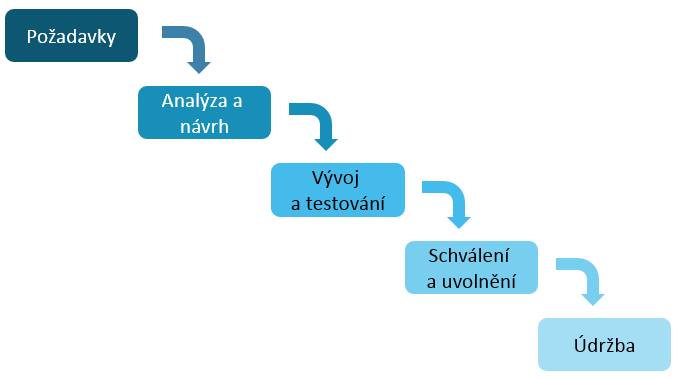
\includegraphics[width=\textwidth]{img/vodopad.png}
    \caption{Vodopádový model \cite{vodopad}}
    \label{img:vodopadimg}
\end{figure}
\FloatBarrier
\subsection{SCRUM}
Metodika s názvem SCRUM je v dnešní době jedna z nejpoužívanějších metodik pro běžný vývoj softwaru. Jedná se o iterativní a inkrementální způsob řízení softwaru, který se řadí mezi agilní metodiky. Jedna z klíčových vlastností je vysoká adaptace na změny zákazníka. Důležitá je také transparentnost. Všichni by měli mít jasný přehled o tom, co a proč se dělá a v jakém je to stavu. Ná obrázku číslo \ref{img:SCRUM} jsou znázorněny hlavní role a činnosti v metodice SCRUM, které budou dále představeny.
\subsubsection{Role}
V metodice SCRUM se vyskytují tři role, které mají za cíl vznik produktu. Při reálném využití SCRUM metodiky mohou být definovány některé další role, ale SCRUM definuje pouze tři následující:
\begin{itemize}
    \item vývojový tým,
    \item vlastníka produktu (product owner),
    \item scrum mastera.
\end{itemize}
Vývojový tým má za úkol dokončit všechny úkoly, které měl v dané iteraci naplánované. Tým musí být soběstačný a každý člen týmu by měl být specialistou na nějakou oblast technologií. Tím je dosaženo, že tým si dokáže poradit s jakýmkoliv problémem. Většinou bývá tým složen z pěti až šesti členů.
\par
Vlastník produktu neboli product owner by měl být zástupce zákazníka. Měl by vědět, co je nutné v další fázi implementovat či změnit. Vlastník produktu je v podstatě komunikační prostředek mezi vývojovým týmem a zákazníkem.
\par
Scrum master je osoba, která dohlíží na správné dodržování metodiky a také má za cíl odstraňování překážek, které brání vývojovému týmu dokončit některé úkoly.\cite{SCRUMImg}
\subsubsection{Události}
V metodice SCRUM se používají čtyři základní události:
\begin{itemize}
    \item iterace,
    \item plánování,
    \item stand-up meeting,
    \item retrospektiva.
\end{itemize}
Iterace nebo také sprint je dopředu ohraničený časový úsek trvající minimálně jeden týden a maximálně jeden měsíc. Nejčastější délka sprintu je okolo dvou týdnů. Za tento časový úsek se snaží vývojový tým vytvořit potencionálně doručitelný produkt (Potentially Shippable Product). Jedná se o produkt, který má alespoň některou svojí část dokončenou a mělo by ho být teoreticky možné zprovoznit v produkčním prostředí zákazníka. Na začátku každé iterace je tzv. plánování a po skončení iterace by měla následovat retrospektiva.
\par
Na začátku každé iterace dochází k tzv. plánování. Jedná se o událost, při které se sejdou všichni členové týmu, scrum master a vlastník produktu. Následně vlastník produktu vybere z backlogu jednotlivé požadavky, které chce v této iteraci dokončit. Backlog je v podstatě soupis všech požadavků, které je nutné zpracovat. Následně vývojový tým konzultuje jednotlivé požadavky vybrané z backlogu a vytváří z nich menší úkoly. Vytvořené úkoly pak ohodnotí časem, jaký by měl stačit k dokončení tohoto úkolu. Po časovém ohodnocení dochází k rozdělení jednotlivých úkolů pro každého člena vývojového týmu.
\par
Stand-up meeting je krátká schůzka vývojového týmu, která se koná každý pracovní den. Délka této schůzky by měla být od 10 do 15 minut. Účelem této schůzky je předat si poznatky mezi celým týmem o rozdělané, hotové či nedokončené práci. Tím se zajistí dostatečná transparentnost ve vývojovém týmu.
\par
Poslední událostí je tzv. retrospektiva. Retrospektiva je schůzka, která se koná po ukončení každé iterace. Na této schůzce probírá tým, jak probíhala práce v uplynulé iteraci, zda je všechno hotové nebo jestli byly nějaké problémy při plnění úkolů. Z retrospektivy mohou vyplynout nějaké další úkoly, které bude nutné v následujících iteracích vyřešit.\cite{SCRUMImg}

\begin{figure}[!htb]
    \centering
    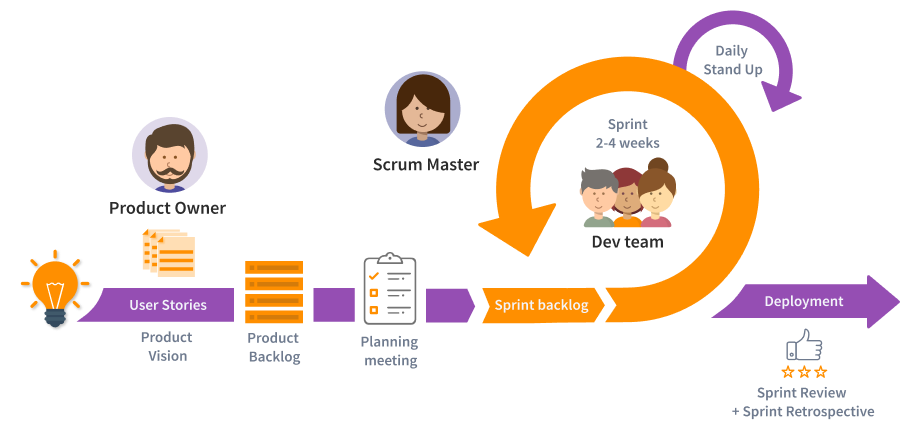
\includegraphics[width=\textwidth]{img/scrum.png}
    \caption{SCRUM proces \cite{SCRUMImg}}
    \label{img:SCRUM}
\end{figure}
\FloatBarrier
\subsection{Extrémní programování}
Extrémní programování je agilní metodikou pro vývoj softwaru, která nespočívá v zavádění nových postupů, ale extremizuje známe postupy či metody, které se osvědčily. Hlavním cílem extrémního programování je co nejrychleji se přizpůsobit na měnící se požadavky ze strany zákazníka, a tím vyvíjet a dodávat kvalitnější software.
\par
V čem spočívá extremizování známých a ověřených postupů? V minulosti se například osvědčila revize programového kódu, tudíž extremizací tohoto postupu je práce ve dvojicích. Ve dvojicích dochází k bezprostřední revizi výsledného kódu, a tím vzniká kvalitnější a lepší programový kód. V minulosti se také osvědčilo testování jednotlivých funkcionalit, takže v extrémním programování dochází k velmi častému testování všeho. V podstatě každý řádek programového kódu by měl být pokrytý testem. Dalším znakem extrémního programování je psát co nejméně složité úseky kódu. Toho lze dosáhnout tím, že implementujeme pouze to, co je v danou chvíli nejdůležitější.\cite{metodiky}
\subsubsection{Postup vývoje}
Extrémní programování funguje podobně jako SCRUM v jednotlivých iteracích. Zákazník může v průběhu iterace doplnit nebo pozměnit požadavky. Pokud k tomuto dojde, tak je prohlášená iterace za ukončenou a začíná se opět od znova. Cyklus vývoje v extrémním programování má nejčastěji následující fáze:
\begin{itemize}
    \item zadávání,
    \item plánování,
    \item designování,
    \item programování,
    \item testování.
\end{itemize}
Nejprve se začne zadáváním, kdy se sepíší jednotlivé případy užití a k tomu odpovídající akceptační scénáře. Jak již bylo zmíněno zákazník může kdykoliv tyto případy užití pozměnit, a tím může dojít k restartu cyklu vývoje.
\par
Další fází je plánování, při kterém se vytvoří časový harmonogram jednotlivých iterací a naplánuje se vydání výsledného produktu.
\par
Fáze designování v sobě zahrnuje návrh jednotlivých funkcionalit, ty se snažíme navrhnout co nejjednodušeji. Nesnažíme se přidávat funkcionality, které zákazník výslovně nepotřebuje.
\par
V fázi programování dochází k implementaci jednotlivých funkcionalit, které se v předchozí fázi navrhnuly. Nejprve dojde k sepsání jednotkových testů a až po té se píše programový kód, který bude testům vyhovovat tzv. vývoj řízený testy (test driven development). Programový kód se píše vždy ve dvojicích, a tím je docíleno jeho vysoké kvality. V rámci této fáze také probíhá integrace jednotlivých částí, kterou provádí vždy pouze jedna dvojice programátorů. Na závěr probíhá optimalizace a úprava vzniklého kódu.
\par
Poslední fází je fáze testování. Jelikož testování je osvědčená metodika pro ověřování kvality softwaru, tak v extrémním programování se testuje všechno a ve velkém množství. Každý úsek programového kódu tedy musí být popsán testem. Pokud se v této fázi vyskytne chyba, tak dojde k opravení a napsání testu na tuto chybu. Dále také vznikají další sady testů, které jsou relevantní pro daný projekt například funkční nebo integrační.\cite{metodiky}
\par
Proces vývoje softwaru pomocí metodiky extrémního programování je zobrazen na obrázku \ref{img:XP}
\begin{figure}[!htb]
    \centering
    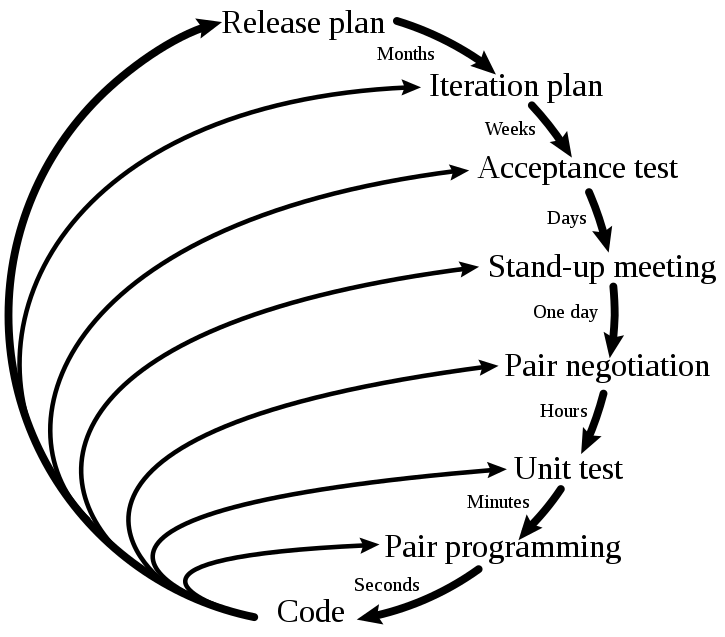
\includegraphics[width=250pt]{img/extremeprogramming.png}
    \caption{Proces vývoje v extrémní programování \cite{metodiky}}
    \label{img:XP}
\end{figure}
\FloatBarrier
\subsection{Kanban}
Kanban je metodika, která se řadí mezi tzv. metody štíhlé výroby. Štíhlá výroba znamená eliminování nadbytečných činností a soustředí se na nejdůležitější faktory, které zákazník opravdu vyžaduje. Tato metoda byla vyvinuta primárně pro výrobní podniky, později se však začala aplikovat i na vývoj softwaru, kde se velice osvědčila. S metodikou SCRUM se řadí mezi nejpoužívanější metodiky v dnešní době.\cite{metodiky}
\subsubsection{Kanban tabule}
V této metodice se klade důraz na vizualizaci. Je tak snadno rozpoznatelné v jaké fázi se nacházejí jednotlivé úkoly. K této vizualizaci se používá tzv. kanban tabule (kanban board). Tato tabule je tvořena jednotlivými sloupci, řádky a úkoly. 
\par
Každý sloupec ukazuje, v jaké fázi se nachází každý úkol. Pokud se změní rozpracovanost daného úkolu, tak se úkol přesune do dalšího sloupce. V této metodice je kladen důraz na omezení počtů úkolů v jednotlivých fázích. V jednom sloupci může být pouze omezený počet úkolů. Tím může nastat problém, že pracovník po dokončení fáze úkolu nemůže přesunout úkol do dalšího sloupce. Avšak díky kanban tabuli je zřejmé, kde nastal problém a mohou pomoci s řešením tohoto problému ostatním členům týmu. 
\par
Řádky na kanban tabuli mohou znázorňovat míru priority jednotlivých úkolů. Čím výše se úkol nachází, tím větší má prioritu a naopak. Úkoly s větší prioritou by měly být plněny přednostně. Prioritu úkolu může určovat nadřízený, ostatní členové týmu nebo přímo zákazník.
\par
Nejčastěji se používá tabule se třemi stavy úkolů: k vyřešení, ve vývoji a dokončené (todo, in progress a done). Avšak tabule může být mnohem složitější a může mít více stavů. Příklad složitější kanban tabule je zobrazena na obrázku číslo \ref{img:kanban_board}. Jednotlivé stavy závisejí na charakteru projektu, který se pomocí kanbanu snažíme dokončit a je možno si je upravovat dle potřeby.
\begin{figure}[!htb]
    \centering
    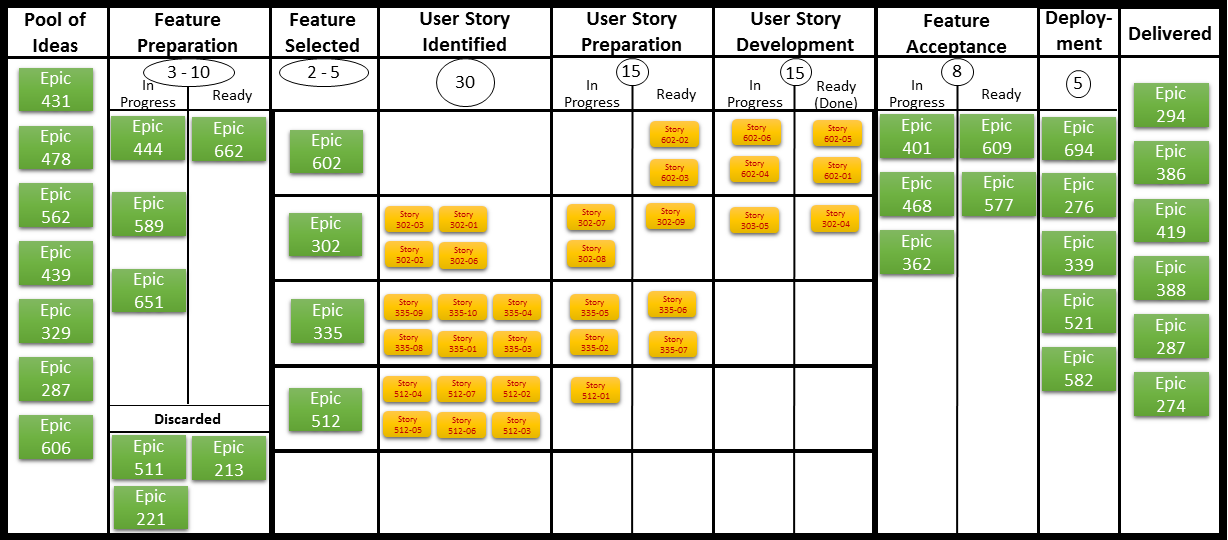
\includegraphics[width=\textwidth]{img/kanban.png}
    \caption{Ukázka kanban nástěnky \cite{metodiky}}
    \label{img:kanban_board}
\end{figure}
\FloatBarrier
\subsection{RUP}\label{sec:rup}
RUP(Rational Unified Process) je metodika vývoje softwaru vyvinutá společností Rational Software Corporation. Tato metodika nebyla vytvořena jako soubor pravidel, která by se měla přísně dodržovat, ale spíše jako soubor doporučení, které si vývojové týmy vybírají podle toho, které odpovídají jejich potřebám. Díky rozsáhlému plánování, analýzám a dokumentaci je vhodnější spíše k řešení větších projektů s velkými týmy. Metodika je velmi komplexní a systematická. Stejně, jako již zmíněný SCRUM, přistupuje k vývoji iterativně, spravuje požadavky zákazníků, ověřuje kvalitu již vytvořených částí softwaru, který vzniká na komponentové architektuře a využívá vizuálního modelování k udržení přehledu nad projektem. \cite{RUPbook}
\subsubsection{Fáze}
Celý proces vývoje softwaru pomocí metodiky RUP můžeme rozdělit do čtyř základních fází:
\begin{itemize}
    \item zahájení,
    \item příprava,
    \item konstrukce,
    \item předávání.
\end{itemize}
Jako první je fáze zahájení. Během počáteční fáze je vytvořen obchodní záměr systému a ohraničen rozsah projektu. K dosažení tohoto cíle musejí být identifikovány všechny externí entity, se kterými bude systém interagovat a
definovat povahu této interakce tzv. případy užití. Definujeme zde kritéria úspěchu, rizika projektu nebo například časový odhad projektu. V této fázi nejvíce komunikujeme se zákazníkem a snažíme se zjistit jeho požadavky.
\par
Hlavním cílem fáze přípravy je analýza problémové oblasti, vytvoření vhodného architektonického návrhu, vypracování projektového plánu. Architektonický návrh musí být navrhnut tak, aby odpovídal jeho rozsahu, hlavním funkcím, ale třeba i mimofunkčním požadavkům, jako jsou
například výkonnostní požadavky.
\par
Během fáze konstrukce jsou implementovány a integrovány všechny komponenty a funkce aplikace, a všechny jeho funkce jsou důkladně otestovány. Jedná se o časově nejnáročnější fázi projektu.
\par
Cílem poslední fáze je předání softwarového produktu zákazníkovi nebo uvedení do provozu. Jakmile je produkt uveden do provozu, tak obvykle vznikají problémy, které vyžadují vývoj opravných verzí.\cite{RUPbook}
\par
Na obrázku číslo \ref{img:RUP} jsou zobrazeny fáze a jednotlivé disciplíny, které se v každé fázi vykonávají a s jakou intenzitou.
\begin{figure}[!htb]
    \centering
    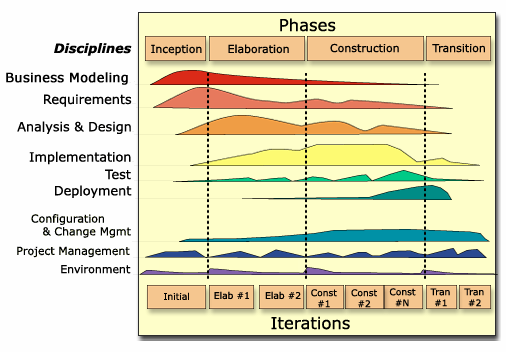
\includegraphics[width=380pt]{img/rup.png}
    \caption{Fáze RUP \cite{RUPbook}}
    \label{img:RUP}
\end{figure}
\FloatBarrier
\subsubsection{Milníky}
Dalším pojmem v metodice RUP jsou tzv. milníky, kterých by se mělo dosáhnout po každé dokončené fází. Jednotlivé milníky jsou:
\begin{itemize}
    \item Lifecycle Objectives,
    \item Lifecycle Architecture,
    \item Initial Operational Capability,
    \item Product Release.\cite{RUPbook}
\end{itemize}
Posloupnost jednotlivých milníků a návaznost na fáze metodiky RUP jsou zobrazeny na obrázku číslo \ref{img:RUP_milestones}.
\begin{figure}[!htb]
    \centering
    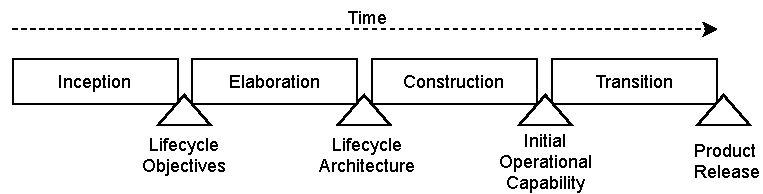
\includegraphics[width=300pt]{img/milestones.pdf}
    \caption{Milníky metodiky RUP}
    \label{img:RUP_milestones}
\end{figure}
\FloatBarrier
% JENDY %
\section{Shrnutí}
V této kapitole byly popsány základní pojmy z oblasti procesu vývoje softwaru. Dále zde byly představeny nejpoužívanější metodiky pro vývoj softwaru. V praxi se často můžeme setkat s některou z uvedených metod, která je však upravena podle potřeb společnosti. Někdy může docházet i ke kombinaci určitých částí jednotlivých metodik.

\chapter{Vzory a Anti-vzory}
Vývoj softwaru je velice složitý a rozmanitý. Při vývoji softwaru můžeme narazit na spoustu problémů, které je nutné pro úspěšné dokončení produktu vyřešit. Jedním z konceptů zabývající se popisem, detekcí a návrhem řešení je problematika tzv. vzorů a anti-vzorů, která je popsána v následující kapitole.

\section{Vzor}\label{sec:pattern}
Ve vývoji softwaru můžeme narazit na spoustu problémů v jednotlivých fázích vývoje. Může se jednat o problém návrhu aplikace, implementace nebo pouze o personální problém. Pokud se tento problém opakuje častěji a je veřejně známý, je možné že existuje nějaké jeho univerzální řešení tzv. vzor. 
\par
Vzor lze definovat jako univerzální řešení známého problému, který můžeme aplikovat stále dokola a tím vyřešit daný problém. Bylo zmíněno, že se jedná o univerzální řešení. Ano v některých případech se může jednat o univerzální řešení, ale ve většině případů je nutné alespoň minimálně daný vzor přizpůsobit naším potřebám.
\par
Vzor lze také definovat jako pojmenovanou dvojici popisu problému a jeho řešení. \cite{antipatterns}

\subsection{Rozdělení vzorů}
Vzory ve vývoji softwaru lze rozdělit do třech základních tříd podle toho, v jaké oblasti problém řeší. Rozdělení je uvedeno v následujícím seznamu:
\begin{enumerate}
    \item architektonické vzory,
    \item designové vzory,
    \item programové vzory.\cite{patterns_classes}
\end{enumerate}
Do první skupiny vzorů můžeme zařadit vzory pro návrh architektury softwaru například přístup klient-server nebo tzv. architektura MVC.
\par
Druhá skupina designové vzory neboli tzv. návrhové vzory, které se využívají k vyřešení známého problému při implementaci softwaru například tzv. singleton (jedináček) nebo factory (tovární metoda).
\par
Poslední skupina vzorů jsou programové vzory, které řeší problémy pro specifické programovací jazyky.
\par
Některé ze zmíněných vzorů jsou popsány v následující sekci číslo \ref{sec:pattern_example}.
\subsection{Příklady vzorů}\label{sec:pattern_example}
\subsubsection{Client-server (klient-server)}
Vzor klient-server řeší problém komunikace a výměny dat mezi jednotlivými instancemi programu. Jedná se v podstatě o síťovou architekturu, která nám definuje několik klientských stanic, které komunikují pomocí různých protokolů se serverem. Server následně řídí komunikaci nebo výměnu dat mezi jednotlivými klienty. Nejčastější klienty si v dnešní době můžeme představit jako webové prohlížeče, kde je zobrazena webová aplikace.
\subsubsection{Factory (tovární metoda)}
Tovární metoda je jeden z nejdůležitějších návrhových vzorů, který umožňuje vyšší abstrakci při vytváření třídy než klasický konstruktor. V praxi se může stát, že potřebujeme vytvořit instanci nějakého objektu a dodatečně ji inicializovat. V tuto chvíli lze využít tzv. tovární metodu, která nám vytvoří instanci daného objektu se základními parametry.
\subsubsection{Singleton (jedináček)}
V programu je někdy nutné sdílet jednu instanci objektu ostatním třídám. Pokud by bylo se v programu vytvářely stále nové instance tohoto objektu, tak by mohlo dojít k přetečení paměti. Proto lze využít vzor s názvem jedináček. Jedináček je tvořen třídou, která se stará o tom, aby instance této třídy existovala pouze jednou. V případě, že je instance této třídy potřeba, nejprve dojde ke kontrole, zda již instance neexistuje. Pokud existuje je vrácena instance této třídy, ale pokud neexistuje vytvoří se nová instance. Praktické využití může být například instance připojení k databázi aplikace.
\section{Anti-vzor}
Pojem anti-vzor (antipattern) lze definovat jako literární forma, která popisuje běžně se vyskytující řešení problému, které má negativní důsledky. Anti-vzor může být špatným výsledkem práce manažera nebo vývojáře, který nemá dostatečné znalosti nebo zkušenosti při řešení daného problému. Špatný výsledek může být také způsoben špatným pochopením řešeného problému.\cite{antipatterns2} Myšlenka anti-vzorů byla zavedena brzy potom, co byl představen koncept vzorů.\cite{antipatterns} V podstatě se jedná o přesný opak vzoru, který byl popsán v předchozí sekci číslo \ref{sec:pattern}.
%\subsection{Struktura anti-vzoru}
%TODO?\cite{antipatterns}
\subsection{Rozdělení anti-vzorů}
Anti-vzory ve vývoji softwaru lze rozdělit opět do třech základních skupin:
\begin{enumerate}
    \item manažerské anti-vzory,
    \item architektonické anti-vzory,
    \item vývojové anti-vzory.
\end{enumerate}
První skupina anti-vzorů je založena na řízení celého projektu, jsou způsobeny jednotlivými manažery nebo vedením. Tyto anti-vzory řeší problémy manažerů, kterým chybí zkušenosti, talent nebo povaha vést
týmy, oddělení nebo organizace. Příklady těchto anti-vzorů jsou například Absentee manager nebo All you have is hammer.\cite{antipatterns}
\par
Další skupinou jsou tzv architektonické anti-vzory, které se zaměřují na nevhodně zvolené strukturu aplikací a jednotlivých komponent. Do této skupiny můžeme zařadit například anti-vzory s názvem Jumble nebo Stovepipe System. \cite{architecture_antipatterns}
\par
Poslední skupinou jsou tzv. vývojové anti-vzory, které se zaměřují přímo na vývoj softwarového produktu. Do této kategorie můžeme zařadit například anti-vzory s názvem Spaghetti Code nebo Big Ball Of Mud.
\subsection{Příklady anti-vzorů}
\subsubsection{Absentee manager}
Tento anti-vzor nastává v případě že má vývojový tým manažera, který není většinu času k dispozici. Pracovníci jsou nucení dělat rozhodnutí bez přítomnosti manažera nebo musejí čekat, až bude k dispozici. Tím může dojít k nejrůznějším problémům jako například opoždění celkového projektu. \cite{antipatterns}
\subsubsection{Stovepipe System}
Anti-vzor který hovoří o špatné integrací více subsystémů. Jednotlivé subsystému jsou napojeny přímo na sebe s žádnou mírou abstrakce. Tím je pak nemožné využít existující rozhraní pro komunikaci s ostatními subsystémy. Navíc je rozhraní silné závislé na dané konfiguraci systému.\cite{architecture_antipatterns}
\subsubsection{Spaghetti Code}
Jedná se o anti-vzor, který označuje nevhodnou strukturu zdrojového kódu, kde každá třída komunikuje s velkým množstvím ostatních tříd. V případě, že uděláme změnu v jedné třídě, dojde k chybám v ostatních třídách. Tím činí výsledný zdrojový kód velice špatně udržitelný a nesrozumitelný.
\section{Shrnutí}
V této kapitole byl představen koncept vzorů a anti-vzorů, jejich základní rozdělení a také některé reálné příklady. Později v práci budou vybrány jednotlivé vhodné anti-vzory, které budou analyzovány. Pro následnou práci je tedy pochopení konceptu anti-vzorů velice důležité.


\chapter{ALM nástroje}
Vysoká konkurence na trhu se softwarovými produkty tlačí jednotlivé dodavatele k co nejrychlejším, bezchybným a kvalitním dodávkám softwaru. K dosažení všech těchto faktorů je možné využít podpůrných nástrojů tzv. ALM (application lifecycle management) nástrojů. Jedná se o nástroje sloužící ke správě životního cyklu aplikace, které zahrnují správu, vývoj a údržbu. Konkrétně se může jednat například o následující činnosti: správa požadavků, návrh softwarové architektury, vývoj, testování, údržba, správa změn, integrace, nasazení nebo správa verzí.
\par
V následující kapitole jsou představeny jednotlivé typy těchto nástrojů a reálné příklady, které se často využívají.
\section{Nástroje pro správu verzí}
Nástroj pro správu verzí nebo také VCS (Version Control System) je systém, který zaznamenává změny souboru nebo sady souborů v čase tak, aby bylo možné se později k potřebné verzi vrátit. Umožní vrátit jednotlivé soubory nebo celý projekt zpět do předchozího stavu, porovnávat změny provedené v průběhu času, zjistit, kdo naposledy upravil něco, co nyní možná způsobuje problémy, kdo a kdy vytvořil diskutabilní část atd.
\par
V dnešní době se můžeme nejčastěji setkat s nástrojem Git. Jedná se o konkrétní systém, sloužící ke správě verzí softwaru. Tento systém se ovládá pomocí příkazového řádku a to může být pro některé uživatele nekomfortní. Často je tedy ovládání integrováno přímo do vývojového prostředí. Další variantou je použití externích nástrojů jako například SourceTree\footnote{\url{http://www.sourcetreeapp.com}}. Dále také existují webové služby, které podporující vývoj softwaru za pomoci verzovacího nástroje Git jako například GitHub\footnote{\url{http://www.github.com}}, GitLab\footnote{\url{http://www.gitlab.com}} atd.
\section{Nástroje pro správu nasazení}
Nástroje pro správu nasazení nové verze produktu jsou převážně označovány zkratkou CI/CD. Tato zkratka představuje spojení kontinuální integrace (continues integration) a kontinuálního doručení (continues delivery). Tyto spojení si lze představit jako dvě fáze.
\par
Fáze kontinuální integrace (CI) je posloupnost kroků, které se provádí při jakékoli změně aplikace. Pokud dojde ke změně v aplikaci, mohlo také dojít k zanesení nových chyb. K ověření správnosti změny dojde v rámci kontinuální integrace k sestavení a otestování všech komponent aplikace. Tím se mohou včasně odhalit jednotlivé chyby a ihned se napravit.
\par
Pokud je ověřena funkčnost výsledné aplikace dochází většinou k nasazení této aplikace do produkčního prostředí. Jedná se často o nahrání nové verze na server, konfiguraci nové verze nebo třeba i o otestování na produkčním prostředí. Je tedy zřejmé, že tato fáze může obsahovat spoustu manuálních kroků, při kterých může vzniknout chyba vlivem lidského faktoru. Nástroje kontinuálního doručení (CD) se snaží všechny kroky spojené s nasazením nové verze automatizovat, a tak i eliminovat možnost vzniku chyb. Proces CI/CD je zobrazen na obrázku číslo \ref{img:cicd}.
\par
K nejčastěji používaným CI/CD nástrojům lze zařadit například Jenkins\footnote{\url{https://www.jenkins.io}}, Travis CI\footnote{\url{https://travis-ci.org}} nebo Circle CI\footnote{\url{https://circleci.com}}. \cite{CICD}
\begin{figure}[!htb]
    \centering
    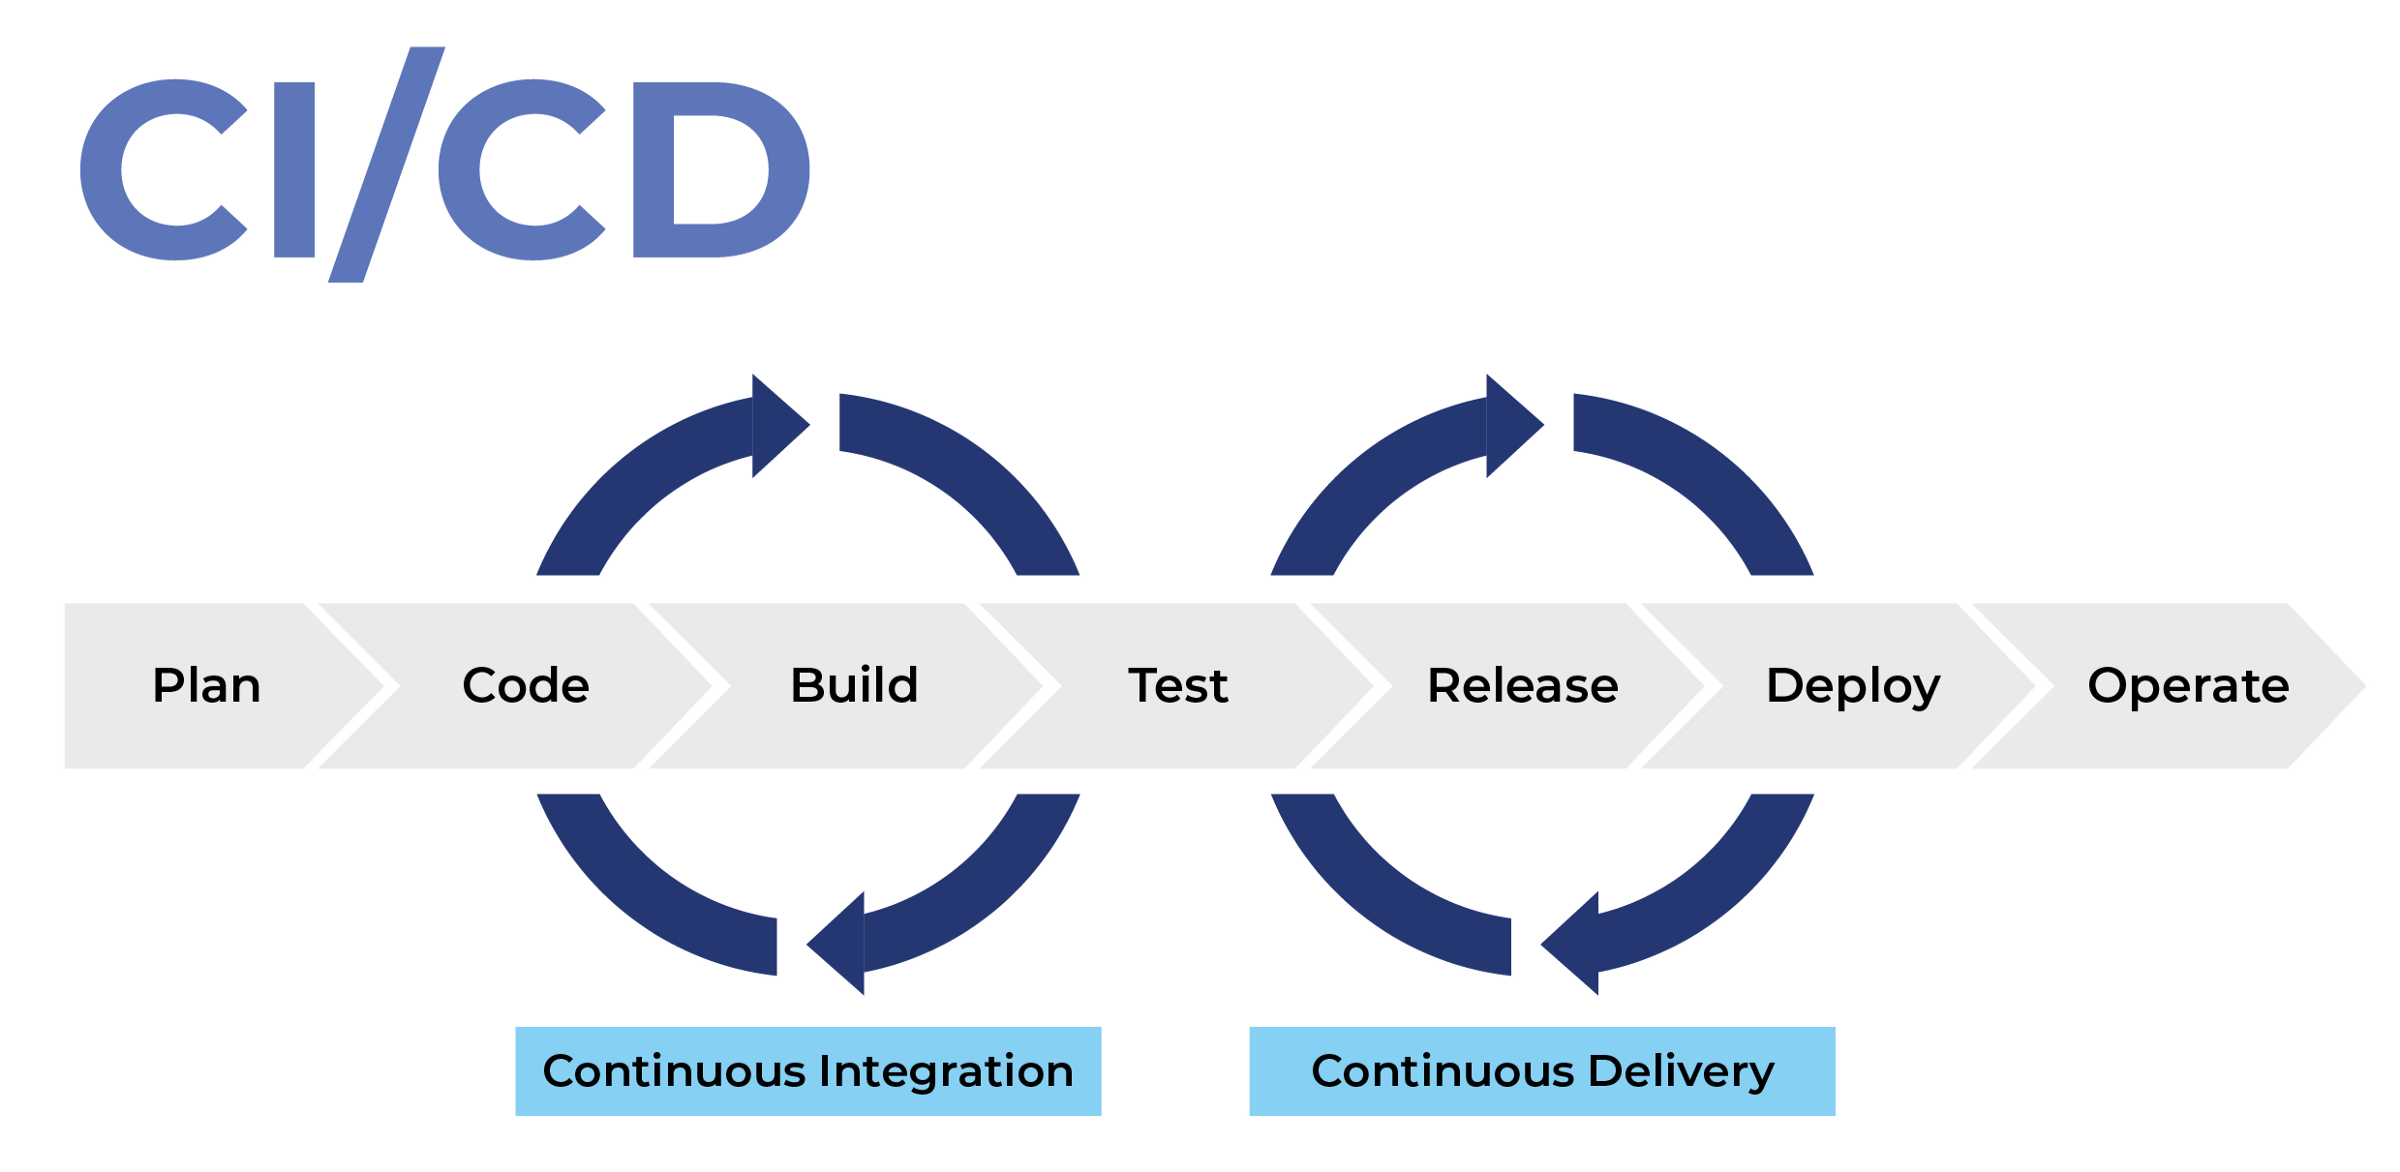
\includegraphics[width=\textwidth]{img/cicd.png}
    \caption{Proces CI/CD \cite{CICD}}
    \label{img:cicd}
\end{figure}
\FloatBarrier
\section{Nástroje pro správu změn a problémů}\label{sec:bugtracker}
Nástroje pro správu změn a problémů se anglicky označují jako issue tracker nebo také bug tracker. Issue lze chápat jako požadavek na změnu, úpravu čí vylepšení produktu. Bug lze chápat jako požadavek na opravu chyby. Tyto nástroje slouží k zajišťování kvality, sledování hlášených softwarových chyb a požadavků při práci programátorů. Tyto nástroje můžeme rozdělit do dvou skupin, a to na veřejné a interní. Do veřejných nástrojů pro správu chyb mohou zadávat chyby koncoví uživatelé. Oproti tomu jsou systémy interní, kam jsou zadávány chyby pouze týmem, který se účastní realizace projektu. Každý záznam se v takovémto systému obvykle nazývá jako tzv. issue, ticket nebo také aktivita.
\par
Aktivita může obsahovat nejrůznější atributy dle povahy projektu. Mezi nejčastější atributy lze zařadit následující:
\begin{itemize}
    \item název,
    \item podrobný popis,
    \item předpokládaná délka řešení aktivity,
    \item dosud odpracovaný čas na aktivitě,
    \item jméno zadavatele,
    \item jméno řešitele,
    \item stav úkolu (např. rozpracovaný, dokončený nebo k řešení).
\end{itemize}
\par
Jedny z hlavních představitelů nástrojů pro správu změn a chyb jsou například Jira\footnote{\url{https://www.atlassian.com/software/jira}}, Redmine\footnote{\url{https://www.redmine.org}} nebo BugZilla\footnote{\url{https://www.bugzilla.org}}. Všechny tyto nástroje obsahují základní správu změn a problémů, ale také obsahují spoustu dalších podpůrných funkcionalit pro komplexní vedení projektu. Mezi tyto funkcionality lze například zařadit tvorbu Gantova diagramu, vedení poznámek o projektu v tzv. wiki, integrace s testovacími nástroji nebo také integrace s nástroji pro správu verzí.
\section{Nástroje pro správu dokumentů}
Jelikož v každém projektu dochází k častým změnám, je zapotřebí tyto změny formálně zanést do příslušných dokumentů.  Pro tento účel by bylo možné využít nástrojů ke správě verzí. Ty jsou však primárně určeny pro programový kód. K tomuto účelu slouží nástroje pro správu dokumentů anglicky označovány jako document management systems zkráceně DMS.
\par
Jedná se o nástroje, které slouží ke správě formálních či neformálních dokumentů souvisejících s projektem.Tyto nástroje lze využít k verzování, úpravě či pouze k nahlížení aktuálně platného dokumentu. V takovýchto systémech jsou také uchovávány informace o tom, kdo dokument, odstavec či úsek textu upravil nebo vytvořil. 
\par
Mezi konkrétní DMS nástroje patří například Google Docs\footnote{\url{https://docs.google.com}}, Dropbox\footnote{\url{https://www.dropbox.com}} nebo Krystal DMS\footnote{\url{https://www.krystaldms.in/}}.
\section{Nástroje pro komunikaci}
Komunikace je jedním ze základních faktorů pro úspěch projektu. Bez dostatečné komunikace se razantně snižuje pravděpodobnost úspěchu projektu. Trendem dnešní doby je řešení většiny problémů distanční formou, tedy za pomocí audio hovorů, video hovorů nebo například pomocí sdílené obrazovky. Tím se dají razantně snížit náklady spojené s cestováním dotyčné osoby.
\par 
Komunikaci můžeme rozdělit na interní a externí. Externí komunikace je prováděna například se zákazníkem nebo dodavatelem. Interní komunikace je prováděna mezi kolegy, v rámci vývojového týmu nebo v rámci celého podniku.
\par
Mezi nejrozšířenější nástroje pro komunikaci patří Microsoft Teams\footnote{\url{https://www.microsoft.com/microsoft-teams}} (nástroj nahrazující Skype), Slack\footnote{\url{https://slack.com}} nebo Google Meet\footnote{\url{https://meet.google.com}}. Nesmíme ale opomenout také elektronickou poštu, která je stále jedním z nejpoužívanějších nástrojů pro komunikaci. Typickým zástupcem nástroje pro elektronickou poštu v podnikové sféře je Microsoft Outlook\footnote{\url{https://www.microsoft.com/microsoft-365/outlook}}.
\section{Shrnutí}
V této kapitole byl představen pojem tzv. ALM nástrojů, základní skupiny těchto nástrojů a konkrétní produkty. 
\chapter{SPADe}\label{sec:spade}
V této kapitole je stručně popsán nástroj SPADe neboli Software Process Anti-pattern Detector, který je vyvíjen na Katedře informatiky a výpočetní techniky (KIV) Fakulty aplikovaných věd (FAV) Západočeské univerzity v Plzni (ZČU). Porozumět tomuto nástroji je z hlediska této práce velice důležité, jelikož bude využit pro analýzu a detekci přítomnosti anti-vzorů v datech nástrojů pro řízení projektů.
\section{Popis nástroje SPADe}
Hlavním cílem nástroje SPADe je dolovat data z různých ALM nástrojů a analyzovat je s ohledem na potenciální přítomnost vzorů a anti-vzorů, jejichž výskyt může negativně ovlivnit průběh projektu nebo výsledného produktu.
\par
V jednotlivých ALM nástrojích jsou uloženy veliké objemy projektových dat, které mezi sebou nejsou vždy logicky propojena. Nástroj SPADe umožňuje dolovat data z jednotlivých ALM nástrojů, následně je mezi sebou logicky uspořádat a uložit do předdefinované struktury ve formě datového skladu. Nad výsledným datovým skladem je lze možno provádět nejrůznější datové analýzy, zobrazovat statistiky projektů nebo například porovnávat vlastnosti podobných projektů, které mohou pomoci ke zvýšení úspěchu daného projektu. Základní struktura nástroje SPADe bude popsána v následující kapitol číslo \ref{sec:spade_struc}.\cite{picha}
\subsection{Struktura nástroje SPADe}\label{sec:spade_struc}
Strukturu nástroje spade lze rozdělit do čtyřech základních částí:
\begin{enumerate}
    \item Dolování dat -- První část pro dolování dat získává z jednotlivých ALM nástrojů pomocí standardního procesu ETL potřebné informace. Každý nástroj má nadefinovaný svůj vlastní proces ETL, jelikož rozhraní jednotlivých ALM nástrojů není jednotné viz podkapitola číslo \ref{sec:datamining}.
    \item Datový sklad -- Pro okamžitou ale i pozdější analýzu získaných dat je zapotřebí uložit výsledná data do datového úložiště. K této funkci slouží datový sklad, který má nadefinovanou strukturu uložených dat a poskytuje získané informace. Struktura datového skladu je popsána v podkapitole číslo \ref{sec:datawarehouse}.
    \item Aplikační vrstva -- Mezivrstva komunikující s prezentační vrstvou a datovým skladem. Zde jsou posílány jednotlivé dotazy do datového skladu a výsledky jsou touto vrstvou následně zpracovány a připraveny pro zobrazení na prezentační vrstvě.
    \item Prezentační vrstva -- S touto částí přímo interaguje uživatel a pomocí této části může uživatel procházet uložená data a zobrazovat si nejrůznější statistiky uložených projektů.
\end{enumerate}
Výše popisovaná struktura nástroje SPADe je graficky zobrazena na obrázku číslo \ref{img:spade_arch}.

\begin{figure}[!htb]
    \centering
    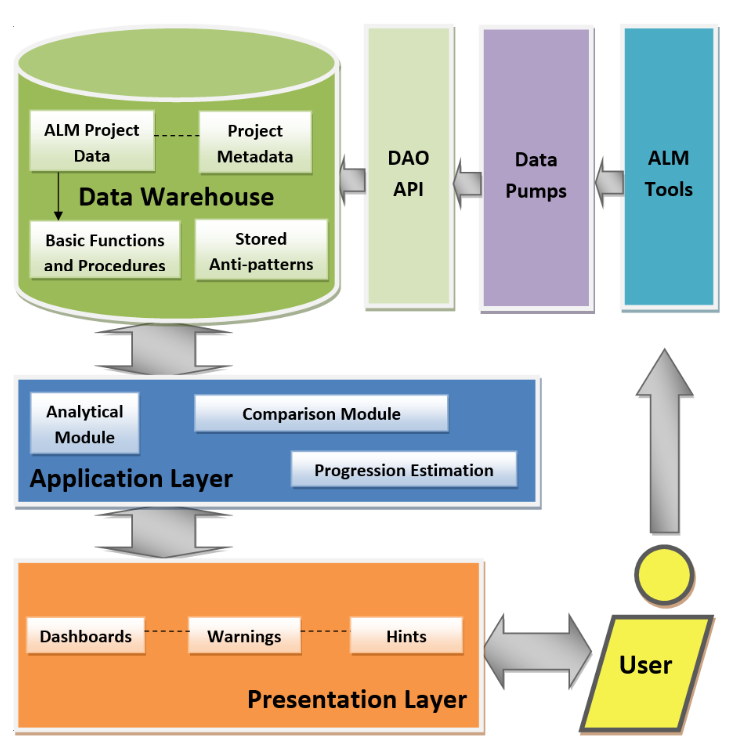
\includegraphics[width=\textwidth]{img/SPADE_arch.png}
    \caption{Architektura nástroje SPADe \cite{picha}}
    \label{img:spade_arch}
\end{figure}
\FloatBarrier
\subsection{Dolování dat}\label{sec:datamining}
Data o každém projektu jsou rozprostřena v různých ALM nástrojích, ze kterých je nutno tyto data získat, zpracovat a uložit do datového skladu nástroje SPADe. Nástroj SPADe umožňuje dolovat data z následujících nástrojů:
\begin{itemize}
    \item Git a SVN,
    \item GitHub,
    \item Bugzilla,
    \item Redmine,
    \item Jira a Assembla.\cite{picha}
\end{itemize}
Dolování dat z jednotlivých nástrojů není vždy unifikované a nelze využít stejný přístup u všech nástrojů. Nejjednodušší přístup dolování dat je přímé připojení do databáze, kde si nástroj ukládá informace. Dalším přístupem je použít tzv. API a pomocí různých dotazů získat potřebná data. Předposledním přístupem je export dat z jednotlivých nástrojů do různých datových formátů (JSON, XML). Následně pak dat zpracovat a uložit do datového skladu. Posledním a nejsložitějším přístupem je přímo přistupovat na uživatelské rozhraní webových ALM nástrojů a pomocí tzv. web crawlingu dolovat potřebná data.\cite{picha}
\section{Datový sklad}\label{sec:datawarehouse}
Datový sklad je systém správy dat, který je navržen k uchovávání velkého množství dat tzv. big data z různých zdrojů. Datový sklad lze následně použít k nejrůznější datovým analýzám. Jeden z největších rozdílů od klasické relační databáze, je že v datovém skladu jsou uloženy i historická data například změny dané instance v průběhu času. \cite{datawarehouse}
\par
Datový sklad nástroje SPADe obsahuje celkem 47 entit, které obsahují komplexní data o jednotlivých projektech získaná z ALM nástrojů zmíněných v kapitole číslo \ref{sec:datamining}. Základní struktura datového skladu je vyobrazena pomocí doménového metamodelu datového skladu nástroje SPADe na obrázku číslo \ref{img:spade_datawarehouse}.
\begin{figure}[!htb]
    \centering
    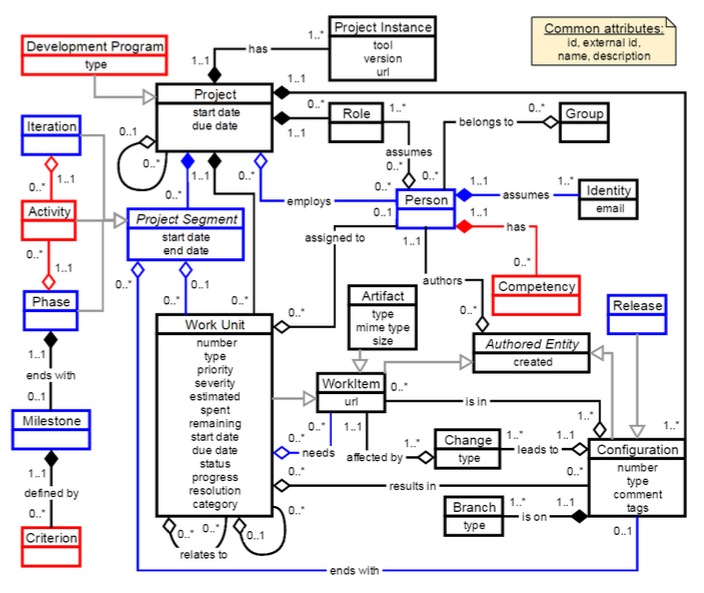
\includegraphics[width=\textwidth]{img/spade_data_model.png}
    \caption{Doménový metamodel datového skladu nástroje SPADe \cite{picha}}
    \label{img:spade_datawarehouse}
\end{figure}
\FloatBarrier
\subsection{Entity}\label{sec:spade_entity}
Jak již bylo zmíněno, v předchozí podkapitole, datový sklad obsahuje celkem 47 entit. Některé nejdůležitější entity jsou popsány v následujícím seznamu:
\begin{itemize}
    \item \texttt{activity} -- Entita obsahující skupinu \texttt{work\_unit}, které spolu souvisí a slučuje je do větších celků s jedním větším cílem.
    \item \texttt{artifact} -- Entita obsahující základní informace o souborech čí adresářích uložených v nástroji pro správu verzí nebo o wiki stránku.
    \item \texttt{configuration} -- Entita obsahující jakýkoliv stav entity \texttt{workItem}, který vyplývá z jakékoli změny entity \texttt{workUnit}. Například commit, nahrání souboru nebo úprava wiki stránky.
    \item \texttt{iteration} -- Entita obsahující informace o jednotlivých iteracích daného projektu. Obsahuje například název iterace, popis iterace, začátek a konec iterace.
    \item \texttt{person} -- Entita obsahující informace o osobě pracující na daném projektu. Dále zde máme entitu \texttt{person\_role}, která udává vztah mezi osobou o rolí v daném projektu.
    \item \texttt{project} -- Entita představující základní informace o jednotlivých projektech. Na tuto entitu je přímo čí nepřímo napojena většina entit v datovém skladu. Obsahuje například název projektu, popis projektu, začátek nebo konec projektu.
    \item \texttt{work\_item} -- Rodičovská entita pro entity \texttt{artifact} a \texttt{work\_unit}. Obsahuje přímou url adresu pro daný záznam například wiki stránku nebo soubor v nástroje pro správu verzí.
    \item \texttt{work\_unit} -- Entita obsahující informace o aktivitě získané z ALM nástrojů. Zde jsou uloženy základní údaje o aktivitě jako například název, autor, odhadovaný a strávený čas. 
\end{itemize}
\subsection{Pohledy}
Samotný datový sklad obsahuje spoustu entit, viz předchozí kapitola \ref{sec:spade_entity}, které jsou mezi sebou propojeny mnoha vazbami. Pro zjednodušení a přehlednější práci obsahuje datový sklad osm pohledů, které spojují několik tabulek do logických celků. Jednotlivé pohledy jsou popsány v následující seznamu.
\begin{itemize}
    \item \texttt{artifactView} -- Data, která zobrazuje tento pohled lze rozdělit na dvě třídy dle atributu s názvem \texttt{artifactClass}. První větší část (\texttt{artifactClass} = "FILE") obsahuje záznamy všech souborů, které byly uloženy v repozitáři příslušného projektu. Druhá menší část (\texttt{artifatClass} = "WIKIPAGE") záznamů obsahuje všechny tzv. wiki stránky\footnote{Jednoduché textové stránky umožnující týmu zaznamenávat potřebné údaje například poznámky ze schůzek.} projektu. U každého záznamu je dále uvedeno například kdo je autorem, k jakému projektu záznam patří, velikost nebo obsah. Kompletní výpis jednotlivých atributů pohledu je zobrazen v tabulce číslo \ref{tab:artifactview}.
    \begin{table}[]
        \begin{tabular}{|l|l|l|}
        \hline
        \textbf{Název atributu} & \textbf{Datový typ} & \textbf{Popis atributu}                              \\ \hline \hline
        \texttt{id}             & bigint(20)          & jednoznačný identifikátor záznamu           \\ \hline
        \texttt{name}           & varchar(255)        & název daného artefaktu                      \\ \hline
        \texttt{description}    & longtext            & obsah daného artefaktu                      \\ \hline
        \texttt{create}         & datetime            & datum a čas vytvoření artefaktu             \\ \hline
        \texttt{url}            & varchar(255)        & umístění artefaktu v projektovém repozitáři \\ \hline
        \texttt{artifactClass}  & varchar(255)        & zda se jedná o soubor nebo o wiki stránku   \\ \hline
        \texttt{mimeType}       & varchar(255)        & typ souboru (php, png, text, html,...)      \\ \hline
        \texttt{size}           & bigint(20)          & velikost artefaktu                          \\ \hline
        \texttt{authodId}       & bigint(20)          & id autora, který artefakt vytvořil          \\ \hline
        \texttt{authorName}     & varchar(255)        & jméno autora, který artefakt vytvořil       \\ \hline
        \texttt{projectId}      & bigint(20)          & reference na projekt                        \\ \hline
        \end{tabular}
        \caption{\label{tab:artifactview}Atributy pohledu \texttt{artifactView}}
    \end{table}

    \item \texttt{personView} -- Pohled umožňující zobrazit jména lidí, která pracují na daném projektu. Kompletní výpis jednotlivých atributů je zobrazen v tabulce číslo \ref{tab:personview}.
    \begin{table}[]
        \begin{tabular}{|l|l|l|}
        \hline
        \textbf{Název atributu} & \textbf{Datový typ} & \textbf{Popis atributu}           \\ \hline \hline
        \texttt{id}             & bigint(20)          & jednoznačný identifikátor záznamu \\ \hline
        \texttt{name}           & varchar(255)        & jméno osoby                       \\ \hline
        \texttt{projectId}      & bigint(20)          & reference na projekt              \\ \hline
        \end{tabular}
        \caption{\label{tab:personview}Atributy pohledu \texttt{personView}}
    \end{table}

    \item \texttt{personWithRolesView} -- Pohled je stejný jako předchozí pohled \texttt{personView}, ale navíc je zde uvedena role každé osoby. Například vývojář, mentor nebo zákazník. Kompletní výpis jednotlivých atributů je zobrazen v tabulce číslo \ref{tab:personroleview}.
    \begin{table}[]
        \begin{tabular}{|l|l|l|}
        \hline
        \textbf{Název atributu} & \textbf{Datový typ} & \textbf{Popis atributu}           \\ \hline \hline
        \texttt{id}             & bigint(20)          & jednoznačný identifikátor záznamu \\ \hline
        \texttt{name}           & varchar(255)        & jméno osoby                       \\ \hline 
        \texttt{projectId}      & bigint(20)          & reference na projekt              \\ \hline
        \texttt{role}           & varchar(255)        & název role dané osoby             \\ \hline
        \texttt{roleClass}      & varchar(255)        & třída role dané osoby             \\ \hline
        \texttt{roleSuperClass} & varchar(255)        & nadřazená třída role dané osoby   \\ \hline
        \end{tabular}
        \caption{\label{tab:personroleview}Atributy pohledu \texttt{personWithRolesView}}
    \end{table}

    \item \texttt{workUnitView} -- Nejdůležitějším pohledem je \texttt{workUnitView}. Tento pohled zobrazuje všechny aktivity, které byly v rámci každého procesu vykonány. Je zde uveden název, popis, autor, řešitel nebo také odhadovaný a skutečný čas aktivity. Výpis nejdůležitějších atributů je zobrazen v tabulce číslo \ref{tab:workunitview}.
    \begin{table}[]
        \begin{tabular}{|l|l|l|}
        \hline
        \textbf{Název atributu} & \textbf{Datový typ} & \textbf{Popis atributu}                         \\ \hline \hline
        \texttt{id}             & bigint(20)          & jednoznačný identifikátor záznamu               \\ \hline
        \texttt{name}           & varchar(255)        & jméno osoby                                     \\ \hline
        \texttt{description}    & longtext        & popis aktivity                                  \\ \hline
        \texttt{dueDate}        & date                & předpokládané datum splnění aktivity            \\ \hline
        \texttt{estimatedTime}  & double              & odhadovaný čas aktivity v hodinách              \\ \hline
        \texttt{spentTime}      & double              & strávený čas na aktivitě v hodinách             \\ \hline
        \texttt{projectId}      & bigint(20)          & reference na projekt                            \\ \hline
        \texttt{autorId}        & bigint(20)         & id autora aktivity                              \\ \hline
        \texttt{assigneeId}     & bigint(20)         & id vykonavatele aktivity                        \\ \hline
        \texttt{iterationName}  & varchar(255)        & název iterace, ve které je aktivita naplánována \\ \hline
        \texttt{statusName}     & varchar(255)        & status dané aktivity                            \\ \hline
        \texttt{priorityName}   & varchar(255)        & název priority dané aktivity                    \\ \hline
        \end{tabular}
        \caption{\label{tab:workunitview}Atributy pohledu \texttt{workUnitView}}
    \end{table}

    \item \texttt{configurationView} -- Pohled poskytující informace o konfiguracích v jednotlivých projektech a o tom, kdo změnu konfigurace provedl. Kompletní výpis jednotlivých atributů je zobrazen v tabulce číslo \ref{tab:configurationview}.
    \begin{table}[]
        \begin{tabular}{|l|l|l|}
        \hline
        \textbf{Název atributu} & \textbf{Datový typ} & \textbf{Popis atributu}           \\ \hline \hline
        \texttt{id}             & bigint(20)          & jednoznačný identifikátor záznamu \\ \hline
        \texttt{name}           & varchar(255)        & název konfigurace                              \\ \hline
        \texttt{type}           & varchar(31)         & o jaký typ konfigurace se jedná                         \\ \hline
        \texttt{description}    & longtext            & popis provedené konfigurace                              \\ \hline
        \texttt{created}        & datetime            & čas a datum vytvoření záznamu                              \\ \hline
        \texttt{authorId}       & bigint(20)          & cizí klíč představující id autora                              \\ \hline
        \texttt{authorName}     & varchar(255)        & jméno autora                              \\ \hline
        \texttt{relationName}   & varchar(255)        & vztah mezi \texttt{authorName} a \texttt{relatedName}                              \\ \hline
        \texttt{relatedId}      & bigint(20)          & identifikátor odpovídající osoby                              \\ \hline
        \texttt{relatedName}    & varchar(255)        & jméno odpovídající osoby                              \\ \hline
        \texttt{projectId}      & bigint(20)          & přiřazení konfigurace k projektu                              \\ \hline
        \end{tabular}
        \caption{\label{tab:configurationview}Atributy pohledu \texttt{configurationView}}
    \end{table}

    \item \texttt{commitedConfigView} -- Tento pohled rozšiřuje předchozí zmíněný pohled \texttt{configurationView} o atribut s názvem \texttt{commited}, který udává, kdy byla konfigurace upravena. Kompletní výpis jednotlivých atributů je zobrazen v tabulce číslo \ref{tab:commitedconfigview}.
    \begin{table}[]
        \begin{tabular}{|l|l|l|}
        \hline
        \textbf{Název atributu} & \textbf{Datový typ} & \textbf{Popis atributu}           \\ \hline \hline
        \texttt{id}             & bigint(20)          & jednoznačný identifikátor záznamu \\ \hline
        \texttt{name}           & varchar(255)        & název konfigurace                              \\ \hline
        \texttt{type}           & varchar(31)         & o jaký typ konfigurace se jedná                              \\ \hline
        \texttt{description}    & longtext            & popis provedené konfigurace                              \\ \hline
        \texttt{created}        & datetime            & čas a datum vytvoření záznamu                              \\ \hline
        \texttt{authorId}       & bigint(20)          & cizí klíč představující id autora                              \\ \hline
        \texttt{authorName}     & varchar(255)        & jméno autora                              \\ \hline
        \texttt{relationName}   & varchar(255)        & vztah mezi \texttt{authorName} a \texttt{relatedName}                              \\ \hline
        \texttt{relatedId}      & bigint(20)          & identifikátor odpovídající osoby                              \\ \hline
        \texttt{relatedName}    & varchar(255)        & jméno odpovídající osoby                              \\ \hline
        \texttt{projectId}      & bigint(20)          & přiřazení konfigurace k projektu\\ \hline
        \texttt{commited}       & datetime            & datum uložení konfigurace tzv. \uv{commit}                              \\ \hline
        \end{tabular}
        \caption{\label{tab:commitedconfigview}Atributy pohledu \texttt{commitedConfigView}}
    \end{table}
    
    \item \texttt{commitView} -- Pohled, který rozšiřuje předchozí pohled \texttt{commitedConfigView}. Pohled obsahuje informace o všech změnách, které byly provedeny v repozitáři každého projektu. U každého záznamu je uvedeno například popis změny (commit message), autor změny nebo do jaké větve (branche) byla změna provedena. Kompletní výpis jednotlivých atributů je zobrazen v tabulce číslo \ref{tab:commitview}.
    \begin{table}[]
        \begin{tabular}{|l|l|l|}
        \hline
        \textbf{Název atributu}& \textbf{Datový typ} & \textbf{Popis atributu}                                  \\ \hline \hline
        \texttt{id}             & bigint(20)      & jednoznačný identifikátor záznamu                             \\ \hline
        \texttt{type}			& varchar(31)  & o jaká typ záznamu se jedná                                                             \\ \hline
        \texttt{name}           & varchar(255)    & jednoznačný idetifikátor commitu                              \\ \hline
        \texttt{description}  	& longtext     & popis daného commitu                                             \\ \hline
        \texttt{created}        & datetime        & datum a čas vytvoření záznamu                                 \\ \hline
        \texttt{authorId}     	& bigint(20)   & id autora commitu                                                \\ \hline
        \texttt{authorName}     & varchar(255)    & jméno autora commitu                                          \\ \hline
        \texttt{relationName} 	& varchar(255) & jméno odpovídající osoby                                                             \\ \hline
        \texttt{relatedId}      & bigint(20)      & identifikátor odpovídající osoby                                                          \\ \hline
        \texttt{relatedName}  	& varchar(255) & vztah mezi \texttt{authorName} a \texttt{relatedName}                                                             \\ \hline
        \texttt{projectId}      & bigint(20)      & reference na projekt                                          \\ \hline
        \texttt{committed}    	& datetime     & datum a čas provedení commitu                                    \\ \hline
        \texttt{isRelease}      & bit(1)          & příznak udávající uvolnění nové verze produktu \\ \hline
        \texttt{tag}          	& varchar(255) & pokud má daný comit tag, tak je uložený zde                      \\ \hline
        \texttt{branch}         & varchar(255)    & název větvě, do které je comitováno                           \\ \hline
        \texttt{main}         	& bit(1)       & příznak udávájící comit do main větve        \\  \hline
        \end{tabular}
        \caption{\label{tab:commitview}Atributy pohledu \texttt{commitView}}
    \end{table}
    
    \item \texttt{fieldChangeView} -- Poslední pohled vychází z pohledu \texttt{configurationView} a obsahuje informace tom, kdy byla konfigurace upravena, jaká byla stará a nová hodnota a jaký \texttt{work\_item} se upravil. Výpis nejdůležitějších atributů je zobrazen v tabulce číslo \ref{tab:fieldchangeview}.
    \begin{table}[]
    	\begin{tabular}{|l|l|l|}
    	\hline
    	\textbf{Název atributu} & \textbf{Datový typ} & \textbf{Popis atributu}           \\ \hline \hline
    	\texttt{id}             & bigint(20)          & jednoznačný identifikátor záznamu \\ \hline
    	\texttt{type}           & varchar(31)         & typ popisující, co bylo změněno                              \\ \hline
    	\texttt{description}    & longtext            & popis příslušné změny                              \\ \hline
    	\texttt{field}          & varchar(255)            & jaké pole bylo změněno                              \\ \hline
    	\texttt{itemId}         & bigint(20)          & id udávající k jaké položce se změna váže                              \\ \hline
    	\texttt{newValue}       & longtext            & nová hodnota příslušného pole                              \\ \hline
    	\texttt{oldValue}       & longtext            & stará hodnota příslušného pole                              \\ \hline
    	\texttt{projectId}      & bigint(20)          & jednoznačný identifikátor projektu                              \\ \hline
    	\texttt{changeName}      & bigint(20)          & popis změny (vytvoření, úprava apod.)                              \\ \hline
    	\end{tabular}
        \caption{\label{tab:fieldchangeview}Atributy pohledu \texttt{fieldChangeView}}
    \end{table}
    
\end{itemize}
\newpage
\section{Shrnutí}
V této kapitole byl popsán nástroj SPADe, jeho struktura, datový sklad atd. Pochopení tohoto nástroje a struktury uložených dat je pro tuto práci velice důležitý, jelikož s využitím tohoto nástroje budou detekovány jednotlivé anti-vzory. V dalších části práce se bude nejčastěji pracovat s jednotlivými pohledy, které zde byly popsány.

\chapter{Návrh detekce anti-vzorů}\label{sec:analyze_detection}
V této kapitole jsou nejprve popsány základní faktory pro výběr vhodných anti-vzorů, které by bylo možné detekovat pomocí nástroje SPADe. Na základě těchto faktorů je vybrána vhodná sada kandidátních anti-vzorů. Jednotlivé anti-vzory jsou zde podrobně popsány a analyzovány pro jejich detekci v projektových datech později v práci.
\section{Výběr vhodných anti-vzorů}
V literatuře lze nalézt veliké množství nejrůznějších anti-vzorů a jejich definic. Nejdůležitějším faktorem pro výběr vhodných anti-vzorů je přítomnost potřebných dat v nástroji SPADe. V případě že nástroj SPADe neobsahuje potřebné informace k vybranému anti-vzoru, je nemožné ho detekovat. Jako příklad zde může sloužit anti-vzor s názvem \textit{Absentee manager}. Tento anti-vzor popisuje negativní dopady absence nebo nedostatečnou komunikaci projektového manažera. Následně mohou nastat situace, kdy musí samotný vývojový tým rozhodovat o něčem, na co nemá kvalifikaci nebo zkušenosti. \cite{antipatterns} Pro detekci tohoto anti-vzoru by bylo nutné mít v datovém skladu uložena data z komunikačních nástrojů.
\par
Dalším faktorem mohou být nekonzistentní data u jednotlivých projektů. Každý tým si v rámci projektu volí své vlastní konvence například používání kategorií, tagů, popis aktivit a pod. Může tedy dojít ke kolizi při používání některých atributů, které jednotlivé týmy používají. Jako příklad zde poslouží anti-vzor s názvem \textit{Indeferent specialist} známý také jako \textit{Domain specialist}. Anti-vzor popisuje člena týmu, který je specialistou pouze na jednu věc a nechce se učit novým věcem mimo jeho specializaci. Často znevažuje ostatní technologii a snižují vážnost věcí, které se nezaobírají jeho specializací. \cite{indiferent_specialist} V tomto případě je velice těžké rozřadit jednotlivé aktivity do doménových specializací, jelikož většina týmů nepoužívá jakékoliv rozřazení.
\par
Dalším faktorem pro výběr vhodných anti-vzorů je absence potřebných dat nejen v nástroji SPADe ale v jakémkoliv jiném ALM nástroji. Jedná se zde o anti-vzory, které lze zařadit do skupiny tzv. osobnostních anti-vzorů (Human anti-patterns). Toto je skupina anti-vzorů, které popisují špatné či nevhodné osobnostní vlastnosti nebo předpoklady dané osoby.\cite{antipatterns} Pro detekci takovýchto anti-vzorů/osob by bylo zapotřebí využít některých sociologických metod a analýzu těchto výsledků pro zjištění takovéto osoby a detekci anti-vzoru.
\par
Dle analýzy známých anti-vzorů na základě předchozích faktorů byla vybrána sada sedmi anti-vzorů, které se budou dále analyzovat v rámci této práce. Sada vybraných anti-vzorů je zobrazena v následujícím seznamu:
\begin{itemize}
    \item Business As Usual,
    \item Long Or Non-Existant Feedback Loops,
    \item Ninety-Ninety Rule,
    \item Road To Nowhere,
    \item Specify Nothing,
    \item Too Long Sprint,
    \item Varying Sprint Length.
\end{itemize}
\section{Popis a návrh detekce pro vybrané anti-vzory}\label{sec:antipattern_analyzation}
V rámci této části bude popsána základní charakteristika každého anti-vzoru, jeho následky a poté bude popsána jeho možná detekce v projektových datech. V rámci každého návrhu detekce bude vždy uvedena jedna či více prahových hodnot. Prahové hodnoty si lze představit jako nastavení striktnosti detekce. Dále bude u každé detekce zobrazen stavový diagram, který přehledně znázorňuje postup detekce daného anti-vzoru.
\subsection{Business As Usual (No Sprint Retrospective)}
\subsubsection{Popis}
Anti-vzor s názvem Business as usual také známý jako No sprint retrospective se zabývá absencí týmové schůzky tzv. retrospektivy po každé iteraci. Po uplynulé a před plánováním následující iterace by mělo dojít ke schůzce celého týmu, kde se celý tým zamyslím na minulou iterací a vytvoří návrhy na zlepšení. Zlepšení jsou představena při plánování následující iterace a na závěr iterace jsou opět vyhodnoceny. \cite{scrum_but_anti_patterns}
\subsubsection{Následky}
Pokud nedochází k retrospektivám po každé iterací, tak nemůže docházet k žádnému vylepšení a změnám při vývoji softwaru. Tím se nemůže zvýšit produktivita vývojového týmu, naopak může spíše klesat. Dále se eliminuje jedna ze základních složek agilního vývoje a to je přizpůsobivost. V případě výskytu tohoto anti-vzoru může vést k několika dalším anti-vzorům, jelikož neexistuje žádný systematický způsob, jak zjisti co funguje a co nefunguje. \cite{scrum_but_anti_patterns}
\subsubsection{Detekce}
Pro detekci tohoto anti-vzoru je nutné se zaměřit na informace o konaných retrospektivách v daném projektu. První variantou je zjistit konání jednotlivých retrospektiv pomocí jednotlivých aktivit. Budeme tedy hledat aktivity, které mohou představovat revizní schůzku týmu pomocí příslušných podřetězců v názvu aktivity. Dále by se dalo zjistit, jestli si na dané aktivitě zaznamenávají čas všichni členové a zda je tato aktivita bez commitu do repozitáře. Na základě další analýzy sady projektových dat však bylo zjištěno, že každý tým má zvolené jiné konvence a zaznamenávat čas na aktivitě může pouze jeden člen týmu za všechny. Tím by se docílilo velkého množství falešných negativních nálezů anti-vzoru. Proto byla zvolena varianta pouze s hledáním retrospektiv pomocí podřetězce v názvu aktivity.
\par
Dále si může tým zaznamenávat poznámky z jednotlivých retrospektiv pouze do wiki stránek. Je tedy zapotřebí nalézt všechny wiki stránky, které v sobě obsahují zmínku o retrospektivě. Jedna wiki stránka může obsahovat poznámky z jedné nebo více retrospektiv. Je tedy nutné se zaměřit na to, kdy byla daná stránka upravena. Tím eliminujeme problém s jednou stránkou pro více retrospektiv.
\par
Nalezené aktivity a wiki stránky následně přiřadíme do jednotlivých iterací. Aktivity jsou přiřazeny podle toho, na jakou iteraci byly naplánovány a wiki stránky jsou přiřazeny k jednotlivým iteracím podle toho, kdy byly upravovány. V ideálním případě by každá iterace měla obsahovat alespoň jednu zmínku o konání retrospektivy. Dále musí být zvolena prahová hodnota (s označením \texttt{X}), která bude představovat minimální počet iterací s detekovanou retrospektivou. Pokud bude minimální počet iterací menší než prahová hodnota je anti-vzor detekován. V opačném případě není detekován. Sekvenční diagram detekce je zobrazen na obrázku číslo \ref{img:business_as_usualas}.
\subsubsection{Prahové hodnoty}
\begin{itemize}
    \item \texttt{X} -- minimální počet iterací s retrospektivou
\end{itemize}
\begin{figure}[!htb]
    \centering
    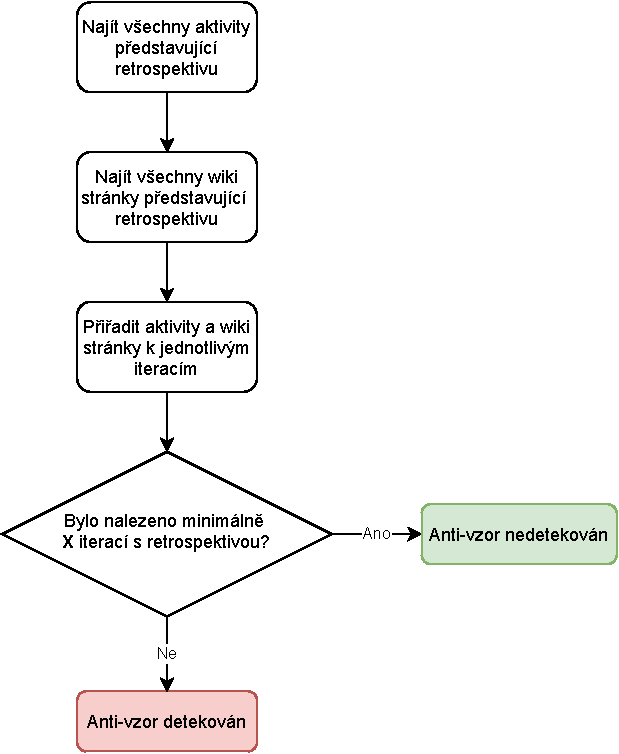
\includegraphics[width=200pt]{img/business_as_usual.pdf}
    \caption{Stavový diagram návrhu detekce pro anti-vzor Business As Usual}
    \label{img:business_as_usualas}
\end{figure}
\FloatBarrier
\subsection{Long Or Non-Existant Feedback Loops}
\subsubsection{Popis}
Tento anti-vzor se zabývá příliš dlouhou nebo vůbec žádnou zpětnou vazbou od zákazníka. Zpětná vazba je jednou z nejdůležitějších faktorů pro úspěšný softwarový produkt. Zpětná vazba by měla být ideálně prováděna po dokončení nějaké větší ucelené části. Nejčastěji může docházet ke komunikaci se zákazníkem po každé vykonané iteraci. Tento problém může být způsoben zhotovitelem nebo zadavatelem projektu. Ze strany zhotovitele se jedná o nedostatečnou nebo nedbalou iniciativu jednotlivých schůzek se zákazníkem. Ze strany zadavatele může nastat problém, kde zadavatel projektu nemá čas nebo zájem vykonávat jakoukoliv zpětnou vazbu zhotoviteli projektu. \cite{scrum_but_anti_patterns}
\subsubsection{Následky}
V případě dlouhé nebo žádné zpětné vazby může docházet k velkým změnám v pozdní fázi vývoje, jelikož zadavatel není s výslednou prací spokojen. Detekce tohoto anti-vzoru může potenciálně představovat spoustu přepracování produktu z důvodu špatného pochopení zákazníka na začátku projektu. Také může vést k vytvoření nesprávných funkcí, které pro zákazníka nemají žádnou hodnotu.
\subsubsection{Detekce}
Pro detekci tohoto anti-vzoru je nutné určit, kdy byly konány schůzky se zákazníkem. Schůzky lze detekovat ze dvou zdrojů. Prvním zdrojem jsou aktivity a druhým zdrojem jsou wiki stránky.
\par
Nejprve jsou nalezeny všechny aktivity, které mohou představovat, dle názvu, schůzku se zákazníkem. Dále tyto aktivity přiřadíme k jednotlivým iteracím. Pokud každá iterace obsahuje alespoň jednu schůzku se zákazníkem, tak není anti-vzor detekován. Toto je ideální případ. V případě že nemá každá iterace detekovanou schůzku se zákazníkem, tak mohou nastav dva případy. Prvním případ je, že tým nezaznamenává schůzky do aktivit a druhý případ je, že se schůzky konaly s velkými rozestupy. Je tedy nutné se rozhodnout od jakého počtu nalezených aktivit se bude hledat ve wiki stránkách a kdy budeme měřit rozestupy mezi schůzkami. Pro tento účel bude sloužit prahová hodnota s označením \texttt{Y1}. Pokud alespoň v \texttt{Y1} iteracích nastala schůzka se zákazníkem, tak dojde k měření rozestupů těchto aktivit. Rozestupy jednotlivých aktivit nesmějí přesáhnout prahovou hodnotu s označením \texttt{Y2}. Stejný rozestup je kontrolovaný mezi začátkem projektu a první schůzkou se zákazníkem. Pokud je překročen tento rozestup, tak je anti-vzor detekován.
\par
V případě že nastala schůzka méně jak v \texttt{Y1} iteracích, dojde k hledání ve wiki stránkách. Musíme tedy najít všechny wiki stránky, které by mohly představovat záznam ze schůzky se zákazníkem (pomocí názvu a obsahu). Jednotlivé wiki stránky přiřadíme k iterací podle data vytvoření nebo upravení. Pokud je u každé iterace nalezena alespoň jedna wiki stránka, není anti-vzor detekován. Dále se zjistí, zda byly nalezeny wiki stránky alespoň v \texttt{Y1} iteracích. Pokud nebyl nalezen dostatečný počet wiki stránek, tak je anti-vzor detekován. Poku byl nalezen dostatečný počet wiki stránek, přichází na řadu měření časového rozestupu mezi úpravami nalezených wiki stránek. Pokud tyto rozestupy nepřesahují délku \texttt{Y2} dní,není anti-vzor detekován.
\par
Sekvenční diagram detekce je zobrazen na obrázku číslo \ref{img:long_or_non_existent_feedback_loops}.
\subsubsection{Prahové hodnoty}
\begin{itemize}
    \item \texttt{Y1} -- minimální počet iteraci, kde se konala alespoň jedna schůzka se zákazníkem,
    \item \texttt{Y2} -- maximální rozestup schůzek se zákazníkem (počet dní).
\end{itemize}
\begin{figure}[!htb]
    \centering
    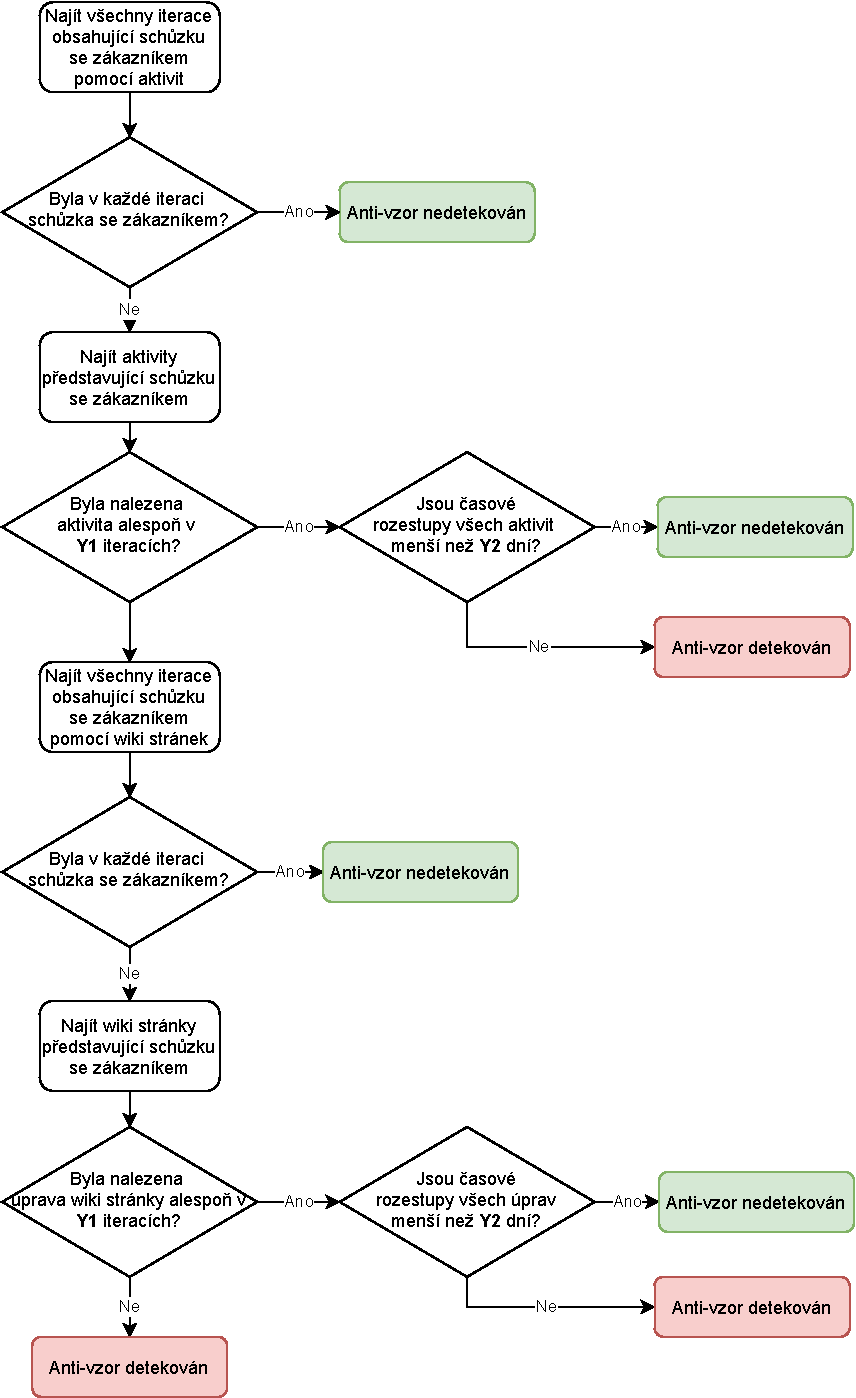
\includegraphics[width=230pt]{img/long_or_non_existent_feedback_loops.pdf}
    \caption{Stavový diagram návrhu detekce pro anti-vzor Long Or Non-Existant Feedback Loops}
    \label{img:long_or_non_existent_feedback_loops}
\end{figure}
\FloatBarrier
\subsection{Ninety-Ninety Rule}
\subsubsection{Popis}
Anti-vzor zabývající se množstvím stráveného času na hotových aktivitách v závislosti na množství času pro dokončení zbylých aktivit. Konkrétní definice tohoto anti-vzoru říká, že 90\% implementačních úkolů zabere 90\% času a zbývajících 10\% implementačních úkolů zabere další 90\% času. Může také nastat situace, že funkcionalita už je skoro hotová, některé aktivity už jsou uzavřené ale stále se čeká pouze na uzavření jedné aktivity, která je však dlouhou dobu otevřena.\cite{ninety_ninety}
\par
Tento anti-vzor může nastat v projektech, kde byla na začátku projektu podceněna nebo chybně provedena analýza náročnosti implementace jednotlivých funkcionalit. Implementace jednotlivých funkcionalit zabere tedy mnohem více, než bylo odhadováno.
\subsubsection{Následky}
Z definice tohoto anti-vzoru vyplývá, že pro finální dokončení produktu bude zapotřebí přibližně o 80\% více času, než bylo plánováno (90\% + 90\% - 100\%). Následkem toho dojde tedy k masivnímu opoždění projektu.
\subsubsection{Detekce}
Detekci tohoto anti-vzoru můžeme rozdělit na dvě části. První částí je analýza stráveného času na implementačních aktivitách na základě definici tohoto anti-vzoru. Konkrétně dochází k rozdělení všech implementačních aktivit (aktivity, které mají commity do repozitáře) v poměru 9:1 dle termínu ukončení. Následně dojde ke spočtení stráveného času u těchto dvou kategoriích, které následně porovnáme. V případě že strávený čas u kategorie s 10\% implementačních aktivit přesáhne strávený čas u kategorie s 90\% implementačních aktivit je anti-vzor detekován.
\par
V opačném případě dochází ke druhému kroku detekce anti-vzoru. Tato detekce je založena na analýze následků tohoto anti-vzoru. Konkrétně následku, který založen na špatných odhadech složitosti jednotlivých implementačních aktivit. Nejprve nalezneme všechny implementační aktivity, které přiřadíme do jednotlivých iterací. Následně spočteme poměr stráveného a odhadovaného času na těchto aktivitách. V průběhu projektu by se měly odhady zpřesňovat a blížit s k hodnotě jedna. Pokud dochází v průběhu projektu spíše ke zhoršování odhadů, je anti-vzor detekován. V opačném případě není anti-vzor detekován.
\par
Sekvenční diagram detekce je zobrazen na obrázku číslo \ref{img:ninety_ninety_rule}.
\begin{figure}[!htb]
    \centering
    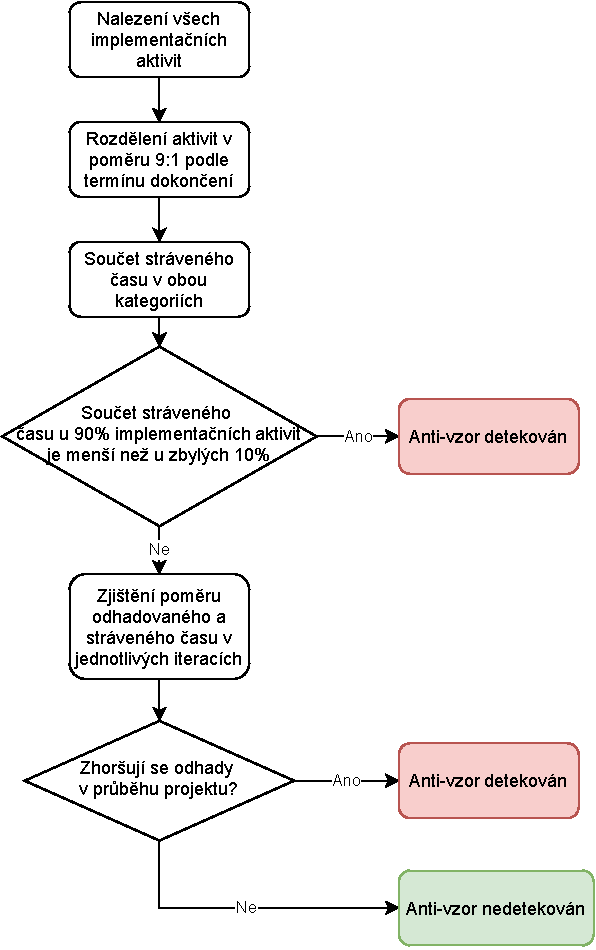
\includegraphics[width=200pt]{img/ninety_ninety_rule.pdf}
    \caption{Stavový diagram návrhu detekce pro anti-vzor Ninety-Ninety Rule}
    \label{img:ninety_ninety_rule}
\end{figure}
\FloatBarrier
\subsection{Road To Nowhere}
\subsubsection{Popis}
Jedná se o anti-vzor, který se zabývá absencí projektového plánu a samotného plánování. \cite{antipatterns2} Projektový plán je dokument, který se sepisuje ve většině případů na začátku projektu. Dokument obsahuje jednotlivé cíle, výstup projektu a jak se k těmto výstupům máme dostat. Projektový plán lze sepsat podle jasně definovaných standardů například PMBOK nebo PRINCE2. Hlavně by měl obsahovat čtyři základní otázky důležité pro projekt a jeho řízení:
\begin{enumerate}
    \item Proč se daný projekt realizuje?
    \item Co je výstupem nebo cílem projektu?
    \item Kdo se na realizaci projektu bude podílet a jaké povinnosti?
    \item Kdy by měl být projekt dokončen a jaké budou jednotlivé milníky? \cite{project_plan}
\end{enumerate}
\subsubsection{Následky}
V případě absence projektového plánu nebo jakéhokoliv plánování může v průběhu projektu docházet ke zmatkům a krizím ve vedení. Pokud není jasně definovaný projektový plán s průběžnými termíny, nejsme schopni vyhodnotit, zda je projekt ve skluzu nebo není. Tím může následně docházet k velikému zpoždění v závěru projektu. Dalším problémem, který může nastat při absenci projektového plánu, je zmatek při vedení projektu. Projektový management neví v jaké části se projekt nachází a na čem se v dané fází má pracovat. Zmatek a chaos se následně může přenést i na vývojový tým, který neví co má dělat a tím klesá i produktivita práce. \cite{antipatterns2}
\subsubsection{Detekce}
Hlavním zdrojem informací pro detekci tohoto anti-vzoru budou informace o aktivitách a wiki stránkách. V prvním kroku detekce je třeba nalézt všechny wiki stránky, které by mohli obsahovat projektový plán. Toho docílíme prohledáváním názvu a obsahu wiki stránek, kde budeme hledat podřetězce připomínající projektový plán. Pokud počet nalezených wiki stránek, představující projektový plán, bude větší nebo rovno prahové hodnotě s názvem \texttt{I1}, není anti-vzor detekován.
\par
Může také nastat situace, kde tým neuložil projektový plán do wiki stránek a vede ho v nějakém externím nástroji. Musíme tedy zjisti, zda existuje nějaká aktivita, která by představovala vytvoření projektového plánu. Projektový plán by měl být ideálně vytvořený na začátku projektu, takže se zaměříme na aktivity v prvních dvou iteracích, které obsahují podřetězec představující vytvoření projektového plánu. Pokud bude počet nalezených aktivit, připomínající vytvoření projektového plánu, větší nebo rovno prahové hodnotě s názvem \texttt{I2}, není anti-vzor detekován. V opačném případě je anti-vzor detekován. Sekvenční diagram detekce je zobrazen na obrázku číslo \ref{img:road_to_nowhere}.
\subsubsection{Prahové hodnoty}
\begin{itemize}
    \item \texttt{I1} -- minimální počet wiki stránek obsahující projektový plán,
    \item \texttt{I2} -- minimální počet aktivit obsahující projektový plán. 
\end{itemize}
\begin{figure}[!htb]
    \centering
    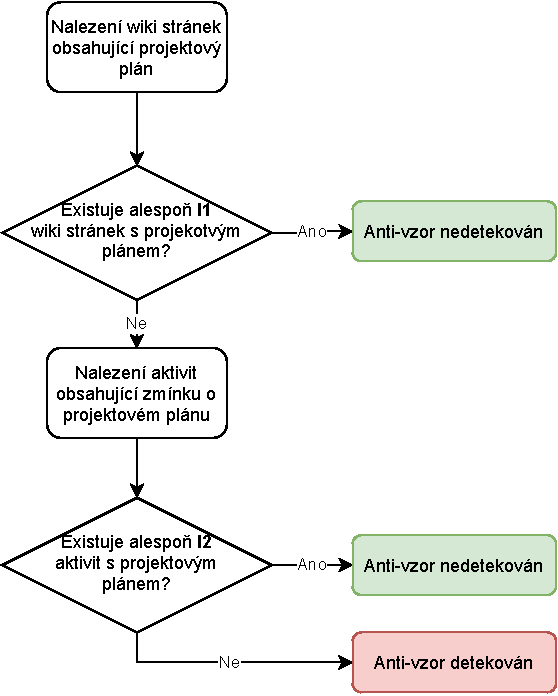
\includegraphics[width=200pt]{img/road_to_nowhere.pdf}
    \caption{Stavový diagram návrhu detekce pro anti-vzor Road To Nowhere}
    \label{img:road_to_nowhere}
\end{figure}
\FloatBarrier
\subsection{Specify Nothing}
\subsubsection{Popis}
Tento anti-vzor se zaobírá problematikou písemné specifikace projektu. V některých organizacích jsou považovány písemné specifikace projektu za naprosto nedůležité a předpokládá se, že členové týmu znají specifikaci projektu zpaměti a není jí nutné sepisovat. V rámci malých projektů a vývojových týmů může tento přístup fungovat. Pokud se však jedná o rozsáhlejší produkty či vývojové týmy, je zcela nemožné vést specifikaci projektu pouze v hlavách členů projektového týmu. \cite{specify_nothing} V některých případech je navíc specifikace projektu závazným dokumentem, na kterém se shodne zadavatel a dodavatel projektu. Proto je písemná forma tohoto dokumenty velice považována za velice důležitou.
\subsubsection{Následky}
Při absenci písemné verze dokumentu specifikace projektu může docházek k rozporům v názorech jednotlivých členů týmu na implementaci dané části produktu. Jelikož neexistuje žádná centrální verze tohoto dokumentu, není možné určit, kdo má pravdu. Výsledkem může být implementace části produktu, která není pro zákazníka vůbec důležitá nebo si ji zákazník představoval jinak.
\par
Dalším problémem, který může nastat jsou personální změny v týmu. Pokud zná specifikaci pouze jeden člen týmu, který se rozhodne tým opustit, je nutné specifikaci předat někomu jinému. Pokud k předání nedojde musí dojít ke schůzce se zákazníkem a specifikaci znovu nadefinovat. Pro zákazníka to může značil neprofesionalitu dodavatele produktu.
\subsubsection{Detekce}
Detekce tohoto anti-vzoru bude rozdělena do třech hlavních částí. V první části se pokusíme nalézt wiki stránky, které představují specifikaci projektu. Toho docílíme hledáním různých podřetězců v názvu či obsahu stránky. Pokud bude počet nalezených aktivit větší nebo roven prahové hodnotě s označením \texttt{J1}, není anti-vzor detekován.
\par
V další části se zaměříme na jednotlivé aktivity projektu. V datovém skladu SPADe nejsou uloženy informace z modulu DMS (Document Management System). Je tedy možné, že byla specifikace vytvořena, ale není o ní žádná zmínka ve wiki stránkách. Toto je možné zjisti pomocí aktivit. Budeme hledat aktivity, které by mohli představovat vytvoření dokumentu specifikace projektu. Specifikace by měla být vytvořena na začátku projektu, omezíme se tedy pouze na aktivity v první a druhé iteraci. Pokud je počet nalezených aktivit větší nebo roven prahové hodnotě s označením \texttt{J2}, není anti-vzor detekován.
\par
V poslední části se zaměříme na průměrnou délku popisu jednotlivých aktivity. Je možné, že si tým nevede strukturovaný dokument, ale specifikaci si uchovává v podobě popisu jednotlivých aktivit. Pokud tedy průměrná délka popisu všech aktivit překročí prahovou hodnotu s označením \texttt{J3}, není anti-vzor detekován, v opačném případě bude detekován. Sekvenční diagram detekce je zobrazen na obrázku číslo \ref{img:specify_nothing}.
\subsubsection{Prahové hodnoty}
\begin{itemize}
    \item \texttt{J1} -- minimální počet wiki stránek představující specifikaci projektu,
    \item \texttt{J2} -- minimální počet aktivit představující tvorbu specifikace projektu,
    \item \texttt{J3} -- minimální průměrná délka popisku aktivity (počet znaků).
\end{itemize}
\begin{figure}[!htb]
    \centering
    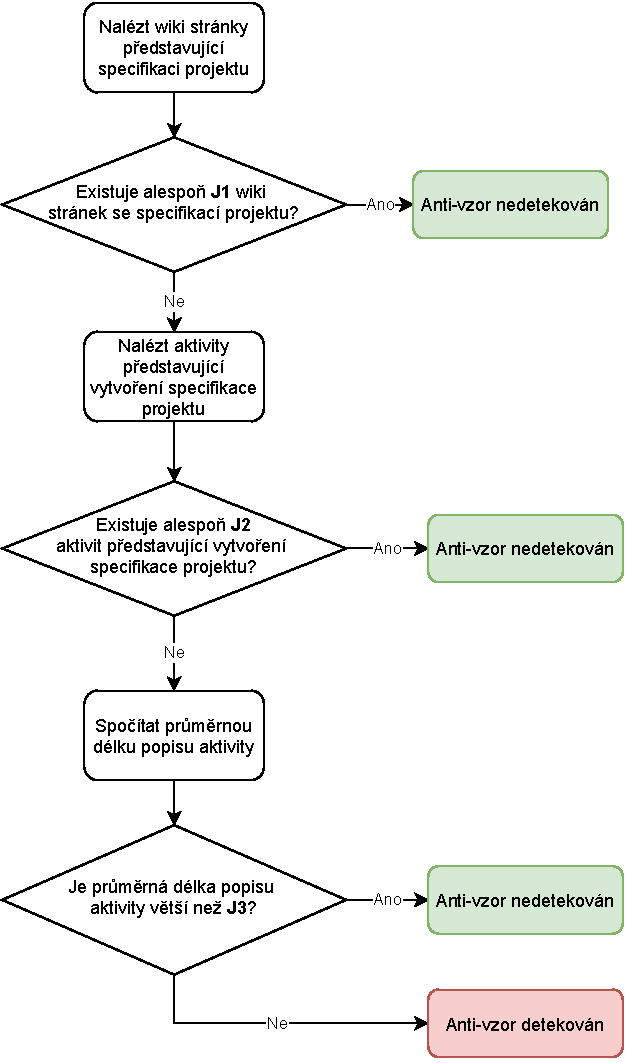
\includegraphics[width=250pt]{img/specify_nothing.pdf}
    \caption{Stavový diagram návrhu detekce pro anti-vzor Specify nothing}
    \label{img:specify_nothing}
\end{figure}
\FloatBarrier
\subsection{Too Long Sprint}
\subsubsection{Popis}
Anti-vzor s názvem Too long sprint se zabývá příliš dlouhými iteracemi. Dle doporučení metodiky SCRUM by měla být délka iterací od dvou do čtyřech týdnů. Pokud bude tato délka překročena, je anti-vzor detekován. \cite{scrum_but_anti_patterns}
\subsubsection{Následky}
Příliš dlouhé iterace svádí k odkládání jednotlivých úkolů na pozdější fázi iterace. Následně je možné, že se na konci iterace nahromadí velké množství nedokončených úkolů, které již není možné dokončit. Další problémem může být špatné dekompozice jednotlivých úkolů. Pro delší iterace se naplánují velké úkoly, které s v průběhu dlouhých iteracích špatně korigují. Na konci iterace se může stát, že byla vytvořena funkcionalita, která neodpovídá zadání od zákazníka. Posledním zásadním problémem může být, pomalá reakce na měnící se priority zákazníka v průběhu projektu. \cite{scrum_but_anti_patterns}
\subsubsection{Detekce}
Pro detekci tohoto anti-vzoru bude pracovat s informacemi o jednotlivých iteracích daného projektu. Nejprve je nutné nalézt všechny iterace pro daný projekt. Dále odebereme první a poslední iteraci z důvodů výkyvů na začátku a na konci projektu. K těmto výkyvům může dojít z časových možností vývojového týmu nebo zadavatele. Výkyvy na začátku a na konci projektu jsou v rámci tohoto anti-vzoru přípustné.
\par
Následně spočteme délku všech iterací pomocí rozdílu data konce a začátku iterace. Pokud jedna ze spočtených délek iterací překročí prahovou hodnotu s označením \texttt{K1}, je inkrementována proměnná pro počet příliš dlouhých iterací. Pokud počet příliš dlouhých iterací přesáhne prahovou hodnotu \texttt{K2}, je anti-vzor detekován. Sekvenční diagram detekce je zobrazen na obrázku číslo \ref{img:too_long_sprint}.
\subsubsection{Prahové hodnoty}
\begin{itemize}
    \item \texttt{K1} -- maximální délka iterace,
    \item \texttt{K2} -- maximální počet příliš dlouhých iterací.
\end{itemize}
\begin{figure}[!htb]
    \centering
    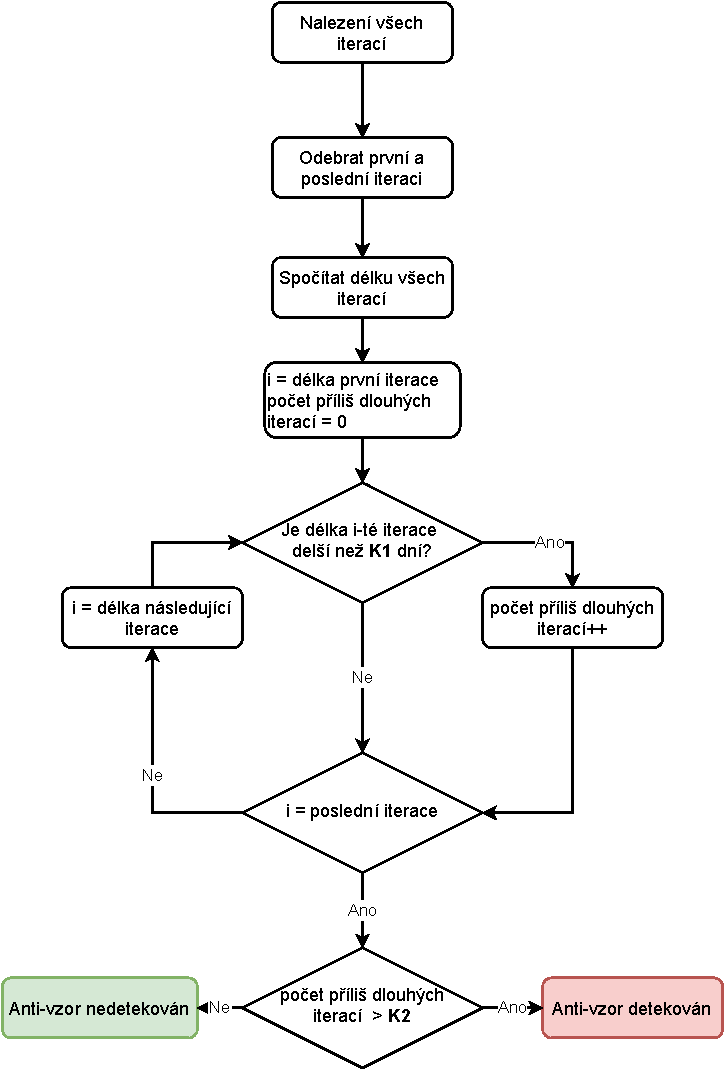
\includegraphics[width=300pt]{img/too_long_sprint.pdf}
    \caption{Stavový diagram návrhu detekce pro anti-vzor Too Long Sprint}
    \label{img:too_long_sprint}
\end{figure}
\FloatBarrier
\subsection{Varying Sprint Length}
\subsubsection{Popis}
Anti-vzor s názvem Varying sprint length se zabývá proměnlivou délkou iterace/sprintu. Délka iterace se v průběhu projektu může měnit, například na základě požadavku vývojového týmu z retrospektivy. Například může dojít k příliš krátké iteraci při inicializaci projektu. Po dokončení první iterace tým následně zjistí, že je iterace příliš krátká a bude lepší jí prodloužit. Toto se může zejména vyskytnou v raných fázích projektu. Opačný případ může nastat před ukončením projektu. Tým zjistí, že dle plánu nestíhá dodat výsledný produkt a dojde ke zkrácení délky iterací. Délka iterace by se však neměla měnit příliš často v průběhu projektu (mimo začátek a konec). \cite{scrum_but_anti_patterns}
\subsubsection{Následky}
Pokud dochází k příliš častým změnám délky jednotlivých iterací v průběhu projektu, je velice obtížné identifikovat dosažení pokroku. Délka jednotlivých iterací může být také prodlužována z důvodu dosažení cílů dané iterace, to může vést ke zpoždění dodání části nebo celého produktu. Zákazník tedy přesně neví, kdy dostane slíbenou část produktu. 
\par
Následek proměnlivé délky iterace také může být odlišná doba konání retrospektivy a plánování iterace. To způsobuje zbytečný čas navíc, které bychom mohli věnovat vývoji samotného produktu. \cite{scrum_but_anti_patterns}
\subsubsection{Detekce}
Pro detekci tohoto anti-vzoru se nejprve naleznou všechny iterace pro daný projekt. Následně se odebere první a poslední iterace, kvůli výkyvům ,které mohou nastat na začátku a na konci projektu. 
\par
Pro zbylé iterace se spočte délka pomocí rozdílu dat konce a začátku iterace. Poté se zkontrolují vždy dvě po sobě jdoucí iterace, pokud bude jejich rozdíl délek větší než prahová hodnota s označení \texttt{L1}, tak dojde k navýšení proměnné pro počet signifikantních změn délek iterace. Po porovnání všech po sobě jdoucích iteracích dojde ke kontrole proměnné pro počet změn. Pokud překročí počet změn prahovou hodnotu s označení \texttt{L2}, je anti-vzor detekován. Sekvenční diagram detekce je zobrazen na obrázku číslo \ref{img:varying_sprint_length}.
\subsubsection{Prahové hodnoty}
\begin{itemize}
    \item \texttt{L1} -- maximální rozdíl délek dvou po sobě jdoucích iteracích (počet dní),
    \item \texttt{L2} -- maximální počet signifikantních změn délek iterace. 
\end{itemize}
\begin{figure}[!htb]
    \centering
    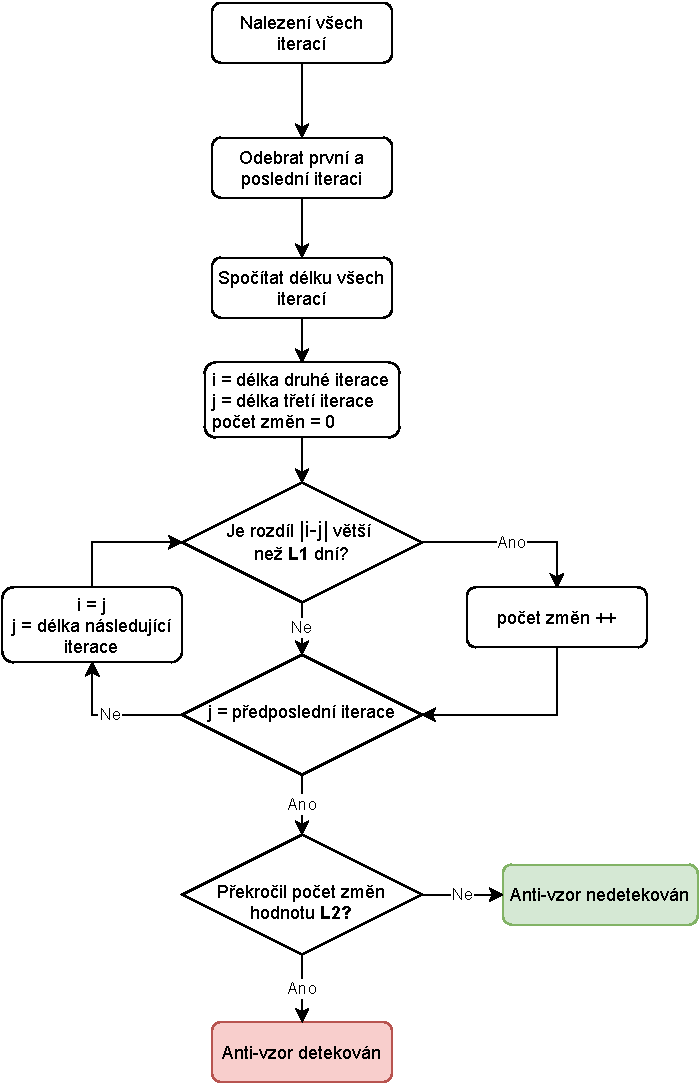
\includegraphics[width=250pt]{img/varying_sprint_length.pdf}
    \caption{Stavový diagram návrhu detekce pro anti-vzor Varying Sprint Length}
    \label{img:varying_sprint_length}
\end{figure}
\FloatBarrier
\section{Návrh pomocné aplikace}\label{sec:app_design}
V rámci detekce jednotlivých anti-vzorů budou získána data z datového skladu SPADe pomocí standardního dotazovacího jazyka SQL. V některých případech by bylo obtížné nebo dokonce i nemožné se omezit pouze na dotazování pomocí SQL. Proto bude detekce anti-vzorů probíhat vždy ve dvou fázích:
\begin{enumerate}
    \item získání potřebných informací z datového skladu SPADe pomocí SQL,
    \item procedurální vyhodnocení získaných informací.
\end{enumerate}
Pro sjednocení rozhraní detekcí všech anti-vzorů a přehledné zobrazení výsledků detekce bude vytvořena pomocná aplikace. Návrh této pomocné aplikace bude popsán v této části.
\subsection{Klíčové vlastnosti}\label{sec:key_properties}
\subsubsection{Čtení z datového skladu SPADe}
Pro detekci jednotlivých anti-vzorů bude zapotřebí získat data, která jsou uložena v datovém skladu. Data budou získávána za pomocí standardních SQL dotazů. Za tímto účelem bude muset být vytvořená komponenta, která zasílá potřebné dotazy do datového skladu a následně zpracuje výsledky dotazů pro následnou analýzu.
\subsubsection{Snadná rozšiřitelnost o další anti-vzory}
V rámci této práce bude implementována detekce pro sedm vybraných anti-vzorů. Cílem vytvoření tohoto nástroje je však snadná rozšiřitelnost o další možné anti-vzory v budoucnu. Proto musí být docíleno co nejsnadnější rozšiřitelnosti o další případné anti-vzory.
\subsubsection{Načítání SQL dotazů ze souborů}
Pro zajištění přehlednosti aplikace bude vhodné SQL dotazy uchovávat v samostatných souborech, které budou součástí výsledné aplikace. Při spuštění detekce dojde k načtení jednotlivých SQL dotazů, do kterých se vloží potřebné atributy. Po připravení dotazu pro detekci dojde k odeslání pomocí modulu pro komunikaci s datovým skladem SPADE.  
\subsubsection{Výběr anti-vzorů a projektů pro analýzu}
Pomocí uživatelského rozhraní přehledně zobrazit všechny dostupné projekty, které jsou uložené v datovém skladu SPADE a všechny implementované anti-vzory. Následně umožnit vybrat uživateli kombinaci projektů a anti-vzorů, které chce detekovat.
\subsubsection{Přehledné zobrazení výsledků}
Hlavním účelem, je přehledně zobrazit výsledky detekce implementovaných anti-vzorů u jednotlivých projektů do tabulky. Dále bude vhodné u každé detekce zobrazit podrobnější informace, na základě kterých byl anti-vzor detekován či nedetekován.
\subsubsection{Nastavení prahových hodnot}
U každého anti-vzoru lze konfigurovat prahové hodnoty, které udávají práh detekce daného anti-vzoru. Nastavení těchto prahových hodnot se může měnit v závislosti na charakteru projektu, aplikace by tedy měla umožňovat jednoduše měnit nastavení těchto hodnot pomocí uživatelského rozhraní nebo pomocí konfiguračního souboru.  
\subsection{Struktura aplikace}
Struktura samotné aplikace byla rozdělena do šesti hlavních částí, které se starají o jednotlivé funkce aplikace.
\par
První část je uživatelské rozhraní, pomocí kterého bude umožněno vybírat jednotlivé projekty a anti-vzory. Následně bude zobrazovat výsledky detekce uživateli.
\par
Druhá část aplikace je tzv. kontrolér, který zpracovává požadavky jednotlivých uživatelů a komunikuje s ostatními moduly. Připravuje data, která budou zobrazena v uživatelské rozhraní.
\par
Další části je modul pro načítání a přípravu sql dotazů. Tento modul zajišťuje načítání potřebných SQL dotazů z příslušných souborů pro detekci. Po načtení vloží do dotazů potřebné atributy jako například identifikační číslo analyzovaného projektu apod.
\par
Po načtení SQL dotazů ze souboru budou zpracovány a odeslány do datového skladu pomocí modulu pro komunikaci s datovým skladem SPADe.
\par
Další část aplikace je modul pro zpracování výsledků jednotlivých dotazů. Tento modul bude transformovat příchozí dat z datového skladu do přívětivějšího formátu, který bude využit dále v aplikaci.
\par
Poslední části aplikace bude modul pro detekci anti-vzorů, který analyzuje výsledná data přijatá od modulu pro zpracování výsledku dotazů. Na základě analýzy získaných dat bude modul rozhodovat o výskytu příslušného anti-vzoru v projektových datech.
\par
Výsledná struktura pomocné aplikace pro detekci anti-vzorů je zobrazena na obrázku číslo \ref{img:app_structure}.
\begin{figure}[!htb]
    \centering
    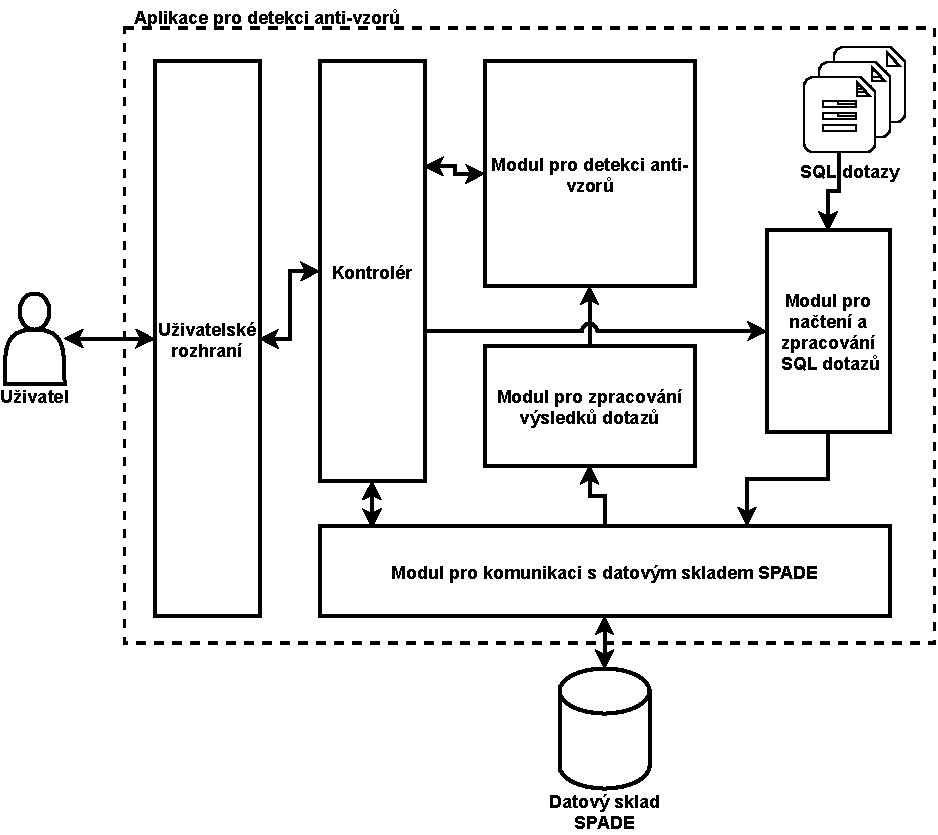
\includegraphics[width=400pt]{img/app_structure.pdf}
    \caption{Návrh struktury aplikace}
    \label{img:app_structure}
\end{figure}
\FloatBarrier
\chapter{Implementace}
V této kapitole bude popsána implementace detekce jednotlivých anti-vzorů na základě analýzy v kapitole číslo \ref{sec:analyze_detection}. Dále zde bude stručně popsána implementace pomocné aplikace pro detekci anti-vzorů.
\section{Implementace detekce anti-vzorů}
Jak již bylo zmíněno v sekci číslo \ref{sec:app_design} detekce anti-vzorů bude probíhat ve dvou krocích:
\begin{enumerate}
    \item získání potřebných informací z datového skladu SPADe pomocí SQL,
    \item procedurální vyhodnocení získaných informací pomocí jazyka Java.
\end{enumerate}
V této části bude popsáno jaké konkrétní pohledy nebo tabulky z datového skladu (popsány v sekci číslo \ref{sec:datawarehouse}) jsou k detekci využívána a k jakému následnému zpracování informací dochází.
\subsubsection{Business As Usual}
Pro detekci tohoto anti-vzoru je nejprve nutné spočíst počet iterací daného projektu. Počet iterací lze zjistit z tabulky s názvem \texttt{iteration}. Jednotlivé iterace jsou vybírány pomocí atributu \texttt{superProjectId}, který odpovídá identifikátoru daného projektu.
\par
V dalším kroku se použije pohled \texttt{workUnitView}, kde jsou vybrány pouze ty aktivity, které mají v názvu podřetězec připomínající retrospektivu například \uv{retr}, \uv{revi} nebo \uv{week scrum}. Následně jednotlivé nalezené aktivity seskupíme pomocí atributu \texttt{iterationName}. Tím dostaneme seznam všech iterací, ve kterých byly nalezeny aktivity připomínající retrospektivu a jejich počet v každé iteraci.
\par
Dalším krokem je pokusit se nalézt jednotlivé wiki stránky, které by mohli obsahovat záznamy z retrospektiv. K tomu budeme zapotřebí pohled \texttt{artifactView}, tabulka \texttt{iteration} a pro detekci změn v jednotlivých wiki stránkách bude zapotřebí pohled \texttt{fieldChangeView}, který je propojen s pohledem pomocí cizího klíče \texttt{itemId}. Artefakty týkající se pouze wiki stránek lze vyfiltrovat pomocí atributu \texttt{artifactClass}, který se rovná hodnotě \uv{WIKIPAGE}. Všechny wiki stránky, které by se mohly týkat retrospektiv jsou detekovány stejným způsobem jako aktivity, s rozdílem, že dochází i ke kontrole obsahu wiki stránky. Tím dostaneme seznam všech změn ve wiki stránkách, které připomínají retrospektivu. Následně pomocí atributu \texttt{fieldChangeView.created} přiřadíme změny k jednotlivým iteracím. Opět tedy získáme seznam všech iterací, ve kterých byla nalezena změna wiki stránky připomínající retrospektivu a počet těchto nálezu v každé iteraci. 
\par
Následně jsou oba výsledně seznamy sloučeny do jednoho. V ideálním případě by každá iterace měla obsahovat alespoň jeden záznam retrospektivy. Počet iterací ve výsledném seznamu je následně porovnám s prahovou hodnotou, která udává minimální počet iterací s retrospektivou. Pokud je počet nalezených iterací s retrospektivou menší než prahová hodnota, je anti-vzor detekován. V opačném případě není detekován.
\subsubsection{Long Or Non-Existant Feedback Loops}
V první kroku detekce dojde k hledání všech iterací, ve kterých proběhla schůzka se zákazníkem. Nejprve jsou nalezeny všechny aktivity pomocí pohledu \texttt{workUnitView}, které by mohly představovat schůzku se zákazníkem. Detekce aktivit probíhám pomocí hledání různých podřetězců v názvu aktivity například \uv{zákazn}, \uv{zadavatel} apod. Následně jsou aktivity seskupeny pomocí atributu \texttt{workUnitView.iterationName}. Pokud byla nalezena aktivita představující schůzku se zákazníkem ve všech iteracích, není anti-vzor detekován.
\par
Pokud nebyla nalezena schůzka se zákazníkem ve všech iteracích, ale alespoň v \texttt{Y1} (minimální počet iterací, kde se konala alespoň jedna schůzka se zákazníkem) iteracích, dochází ke kontrole rozestupů těchto aktivit/schůzek. U první a poslední a první nalezené schůzky ještě probíhá kontrola rozestupu od začátku a konce projektu. Začátek a konec projektu je zjištěn z tabulky \texttt{iteration}. Začátek projektu je detekován pomocí atributu \texttt{iteration.startDate} u první iterace a konec projetu je detekován pomocí atributu \texttt{iteration.endDate} u poslední iterace. Pokud překročí rozestup schůzek se zákazníkem prahovou hodnotu \texttt{Y2} (maximální rozestup schůzek se zákazníkem), tak je anti-vzor detekován.
\par
Pokud není nalezen potřebný počet aktivit, je možné, že tým zaznamenává schůzky pouze do wiki stránek. Za pomocí pohledu \texttt{artifactView} jsou nalezeny všechny aktivity, které by mohly připomínat schůzku se zákazníkem. V případě, že má tým vytvořenou pouze jednu wiki stránku pro všechny schůzky, je navíc využito pohledu \texttt{fieldChagneView}, pomocí kterého lze zjistit změny v nalezených wiki stránkách v průběhu projektu. Akceptovatelné změny jsou pouze ty, kde je délka nového obsahu wiki stránky delší než starého obsahu (\texttt{length(newValue) > length(oldValue)}).
\par
Pokud jsou nalezené wiki stránky ve všech iteracích, není anti-vzor detekován. V opačném případě dochází ke kontrole rozestupů úprav jednotlivých wiki stránek. Kontrola rozestupu opět probíhá i s porovnám vůči začátku a konci projektu. V případě, že některý rozestup překročí prahovou hodnotu \texttt{Y2} (maximální rozestup schůzek se zákazníkem), je anti-vzor detekován.
\subsubsection{Ninety-Ninety Rule}
TODO
\subsubsection{Road To Nowhere}
Pro detekci tohoto anti-vzoru je nejprve nutné u každého projektu nalézt první dvě iterace. Toho docílíme pomocí tabulky \texttt{iteration}, kde jednotlivé iterace seřadíme pomocí atributu \texttt{iteration.startDate} a po té vybere operátorem \texttt{LIMIT} a \texttt{OFFSET} první dvě iterace.
\par
Dalším krokem je nalezení všech wiki stránek představující projektový plán, který byl vytvořen v první nebo druhé iteraci. S využitím pohledu \texttt{artifactView} nalezneme všechny wiki stránky pomocí atributu \texttt{artifactClass} = \uv{WIKIPAGE}. Následně dojde k hledání podřetězce v názvu nebo obsahu wiki stránky představující projektový plán.
\par
V dalším kroku je nutné nalézt všechny aktivity, které byly dokončeny v první nebo druhé iteraci a mohly by představovat vytvoření projektového plánu. Pomocí pohledu \texttt{workUnitView} nalezneme všechny aktivity v první a druhé iteraci. Pohled \texttt{workUnitView} neobsahuje id iterace, kontrola, zda aktivita spadá do první nebo druhé iterace, je tedy prováděna za pomocí atributu \texttt{workUnitView.iterationStartDate}. Dále je zapotřebí detekovat aktivity týkající se projektového plánu. Tyto aktivity jsou detekovány pomocí hledání podřetězce v názvu nebo popisku.
\par
V poslední fázi dochází nejprve k porovnání počtu nalezených wiki stránek s prahovou hodnotou, která udává minimální počet těchto stránek. Pokud není nalezena žádná stránka, je porovnán počet nalezených aktivit s prahovou hodnotu, která udává minimální počet těchto aktivit. Pokud není ani v jednom případě detekován potřebný počet, je anti-vzor detekován. V opačném případě není detekován.

\subsubsection{Specify Nothing}
Detekci anti-vzoru Specify nothing lze rozdělit do čtyřech hlavních části. V první části je nutné zjistit, zda se v projektových datech vyskytuje samotný dokument specifikace projektu. Toho můžeme docílit pomocí pohledu \texttt{artifactView}, pomocí kterého vyhledáme všechny wiki stránky potenciálně představující specifikaci projektu. Wiki stránky jsou detekovány pomocí podřetězce v názvu například \uv{DSP} nebo \uv{specification}.
\par
Jak již bylo zmíněno v analýze, samotný dokument specifikace projektu může být veden v některém externím nástroji pro správu dokumentů. Proto je nutné se dále zaměřit na pohled \texttt{workUnitView}, který představuje aktivity projektu. Je nutné detekovat aktivity, které by mohly představovat vytvoření specifikačního dokumentu.
\par
Dále je nutné se zaměřit na průměrnou délku popisku jednotlivých aktivit. Popisky aktivit jsou uloženy v atributu \texttt{workUnitView.description} a pomocí standardní SQL funkce \texttt{AVG()} je spočtena průměrná délka popisku.
\par
Po získání všech potřebných informací z datového skladu jsou jednotlivé počty nalezených wiki stránek, aktivit a průměrné délky textu popisku aktivit porovnány s prahovými hodnotami. V případě že jsou všechny nalezené položky pod prahovými hodnotami, je anti-vzor detekován.
\subsubsection{Too Long Sprint}
Pro detekci tohoto anti-vzoru je zapotřebí pouze jedné tabulky s názvem \texttt{iteration}. Nejprve dojde k detekci první a poslední iterace, které v detekci nebudou figurovat z důvodu možných výkyvů na začátku a konci projektu.
\par
Následně dojde ke spočtení délek všech zbylých iterací pomocí atributů \texttt{iteration.startDate} a \texttt{iteration.endDate} s využitím standardní SQL funcke \texttt{DATEDIFF()}. Tím získáme délku jednotlivých iterací ve dnech.
\par
Dále dochází ke kontrole každé délky iterace a pokud překročí délka jedné iterace prahovou hodnotu (prahová hodnotu udává maximální délku iterace), je navýšena proměnná \texttt{numberOfLongIterations}. Pokud překročí proměnná \texttt{numberOfLongIterations} prahovou hodnotu udávající maximální počet příliš dlouhých iterací, je anti-vzor detekován.
\subsubsection{Varying Sprint Length}
K detekci tohoto anti-vzoru bude zapotřebí získat informace o délkách jednotlivých iteracích. Proto bude první fáze implementace detekce tohoto anti-vzoru totožná s detekcí anti-vzoru Too long sprint.
\par
Po získání délek všech iteracích (kromě první a poslední) dochází k porovná vždy dvou po sobě jdoucích iteracích. Pokud rozdíl jejich délek překročí prahovou hodnotu (maximální změna délky iterace) je navýšena proměnná \texttt{iterationLengthChanged} o jedničku. Pokud po porovnání všech dvou po sobě jdoucích iterací bude proměnná \texttt{iterationLengthChanged} větší než prahová hodnota udávající maximální počet změn délek iterací, je anti-vzor detekován. V opačném případě není detekován.
\section{Implementace pomocné aplikace}
V této části bude popsána implementace pomocné aplikace pro detekci anti-vzorů, která byla navrhnuta v předchozí kapitole.
\subsection{Zvolené technologie}
Aplikace pro detekci anti-vzorů je implementována jako jednoduchá webová aplikace. Důvody pro vytvoření webové aplikace byly následovné:
\begin{itemize}
    \item trend dnešní doby,
    \item snadný přístup k aplikaci bez nutnosti instalace na každé zařízení,
    \item snadná implementace REST API v případě potřeby propojení aplikace s ostatními webovými službami. 
\end{itemize}
Jelikož se jedná o velmi malou aplikaci je implementována monolitickou architekturou (uživatelské rozhraní není samostatně stojící služba).
\par
Pro implementaci bylo využito populárního open-source frameworku s názvem Spring. Jedná se o aplikační rámec neboli framework pro vývoj J2EE aplikací. Uživatelské rozhraní je implementováno pomocí jednoduchého šablonovacího systému s názvem Thymeleaf.
\par
Pro komunikaci s datovým skladem, který je uložen v MySQL databázi bylo využito standardního JDBC konektoru pro komunikaci s MySQL databázemi.
\subsection{Struktura projektu}
Struktura a popis jednotlivých složek či souborů aplikace je zobrazen v tabulce číslo \ref{table:struktura_aplikace}. Znak * nahrazuje cestu \texttt{src/main} a znak \texttt{\#} nahrazuje složku \texttt{resources} z důvodu úspory místa v tabulce.
\begin{table}[ht]
	\caption{Struktura projektu aplikace} % title of Table
	\centering % used for centering table
	\begin{tabular}{l l } % centered columns (4 columns)
		\textit{Složka/Soubor} &  \textit{Obsah}  \\ [0.5ex] % inserts table
		%heading
		\hline % inserts single horizontal line
		\texttt{*/java} & zdrojové kódy aplikace,  \\
		\texttt{*/\#/application.properties} & nastavení aplikace,  \\
		\texttt{*/webapp/queries} & definice dotazů pro anti-vzory,  \\
		\texttt{*/webapp/WEB-INF/templates} & html šablony uživatelského rozhraní,  \\
		\texttt{pom.xml} & soubor pro sestavení aplikace,  \\	
		\texttt{db\_dump.sql} &  soubor pro obnovu datového skladu,  \\
		\texttt{docker-compose.yml} & soubor pro spuštění aplikace v Dockeru.  \\	
		\hline %inserts single line
	\end{tabular}
	\label{table:struktura_aplikace} % is used to refer this table in the text
\end{table}
\FloatBarrier
\subsection{Balíky tříd}
Jednotlivé třídy jsou děleny do tzv. balíků. Balíky tříd jsou umístěny ve složce \texttt{cz.zcu.fav.kiv.antipatterndetectionapp}. V této složce je také umístěna hlavní třída s názvem \texttt{AntiPatternDetectionAppApplication}, která zajišťuje spuštění celé aplikace. Třídy jsou do jednotlivých balíků rozděleny podle funkce dané třídy. Celkem je projekt tvořen sedmi balíky, které jsou níže popsány.
\begin{itemize}
    \item \texttt{controller} -- Balík obsahuje pouze jednu třídu, která představuje kontrolér aplikace. Tento kontrolér zpracovává požadavky jednotlivých uživatelů a následně zobrazuje data do uživatelského rozhraní.
    \item \texttt{detecting} -- Balík obsahující všechny potřebné třídy pro detekci jednotlivých anti-vzorů a připojení k datovému skladu SPADe.
    \item \texttt{model} -- Balík obsahující modelové třídy nebo také tzv. přepravky pro snadné předávání dat v rámci jednotlivých komponent aplikace.
    \item \texttt{repository} -- Balík obsahující jednotlivé komponenty, které se starají načítání a ukládání načtených SQL dotazů ze souborů a inicializaci jednotlivých detektorů anti-vzorů.
    \item \texttt{service} -- Balík obsahující jednotlivé služby pro práci s instancemi jednotlivých projektů a anti-vzorů.
    \item \texttt{spring} -- Třídy obsahující konfiguraci frameworku Spring pro korektní fungování webové aplikace. Například ve třídě \texttt{AppConfig} je definováno, kde jsou uloženy šablony pro uživatelské rozhraní.
    \item \texttt{utils} -- Balík obsahující pouze jednu třídu \texttt{Utils}, která obsahuje pomocné statické metody používané na různých místech v aplikaci.
\end{itemize}

\subsection{Rozšíření o další anti-vzory}
Pro zajištění co nejjednoduššího rozšíření o další detekce anti-vzorů jsou pomocí reflexe automaticky načítány všechny třídy, které implementují rozhraní s názvem \texttt{AntiPatternDetector}. Poté je volána přímo metoda s názvem \texttt{analyze}, která analyzuje vybraný antivzor.
\par
Pro rozšíření aplikace o další anti-vzor je nutné provést následující dva kroky:
\begin{enumerate}
    \item implementovat rozhraní \texttt{AntiPatternDetector} a všechny jeho metody,
    \item vytvořit soubor s SQL dotazy ve složce \texttt{/src/main/webapp/queries}.
\end{enumerate}
Rozhraní obsahuje čtyři metody, které je nutné implementovat. Funkce jednotlivých metod je popsána v následujícím seznamu:
\begin{itemize}
    \item \texttt{getAntiPatternModel} -- metoda vracející instanci modelové třídy anti-vzoru pro zobrazení v uživatelském rozhraní (v této modelové třídě lze také definovat prahové hodnoty daného anti-vzoru),
    \item \texttt{getAntiPatternSqlFileName} -- metoda, která vrací název souboru s sql dotazy pro daný anti-vzor,
    \item \texttt{setSqlQueries} -- motoda, která nastavuje SQL dotazy načtené ze souboru k tomuto anti-vzoru (k načítání dochází pouze jednou a to pří startu aplikace), 
    \item \texttt{analyze} -- metoda, která pracuje s výsledky SQL dotazů a provádí konečnou detekci anti-vzoru.
\end{itemize}
Pro správné fungování detekce je nutné zachovat jednotnou formu souborů s SQL dotazy. Každý dotaz musí být na samostatné řádce a musí být ukončen středníkem.
\chapter{Experiment}
V této kapitole je proveden experiment detekce implementovaných anti-vzorů na vybrané sadě projektových dat. Výsledky jsou následně diskutovány a jsou zde uvedeny možná rozšíření jednotlivých detekcí.
\section{Postup experimentu}
Experiment bude rozdělen do následujících částí:
\begin{enumerate}
    \item výběr vhodné sady projektů,
    \item nastavení prahových hodnot pro jednotlivé anti-vzory,
    \item provedení detekce,
    \item vyhodnocení výsledků,
    \item diskuze výsledků.
\end{enumerate}
\section{Výběr vhodné sady projektů}
Výběr vhodných projektů je pro úspěch detekce anti-vzorů velice důležitý. Musí být k dispozici dostatečné množství informací o každém projektu, o jednotlivých aktivitách, iteracích ale také o různých artefaktech. V případě, že by projektová data obsahovala malé množství těchto informací, může dojít ke špatné detekci jednotlivých anti-vzorů. K dispozici se nabízejí tři varianty zdrojů projektů, respektive projektových dat:
\begin{enumerate}
    \item komerční projekty,
    \item open source projekty,
    \item interní projekty Katedry informatiky a výpočetní techniky na ZČU.
\end{enumerate}
První zmíněnou skupinou jsou komerční projekty. Jedná se o softwarové projekty tvořené softwarovými společnostmi, které produkují buď vlastní produkty nebo produkty na základě zákaznické poptávky. Každá softwarová společnost používá některé metodiky pro vývoj softwaru, které si přizpůsobuje svým vlastním potřebám. Tím si v podstatě tvoří svoje vlastní know-how pro vývoj softwaru. Tímto know-how si vytváří konkurenční výhodu oproti ostatní společnostem, které jsou na trhu. Proto je velice složité tyto data od komerčních společností získat a pro účely této práce nebudou využita.
\par
Další skupinou jsou tzv. open source projekty. Jedná se o projekty s veřejně přístupným zdrojový kódem a každý vývojář může buď přispět k vývoji tohoto produktu nebo si může produktu upravit pro své vlastní potřeby. Tento typ projektů je sice veřejně dostupný, ale ve většině případů je dostupný pouze zdrojový kód aplikace. V lepším případě je dostupný přímo repozitář daného projektu, takže můžeme vidět jednotlivé změny v průběhu času tzv. commity. Z těchto informací by bylo možné detekovat jen velice malou omezenou část anti-vzorů a proto nebudou pro detekci v této práci vybrána. K potřebám této práce bychom potřebovali znát více informací z dalších ALM nástrojů, jako například z nástrojů pro správu změn a problémů popsané v kapitole číslo \ref{sec:bugtracker}.
\par
Poslední skupinou jsou interní projekty, které jsou vytvářeny na Katedře informatiky a výpočetní techniky Fakulty aplikovaných věd Západočeské univerzity v Plzni. Konkrétně se jedná o projekty, které jsou vytvářeny v rámci předmětu pokročilého softwarového inženýrství (ASWI). V rámci těchto projektů se využívá metodika přizpůsobena pro tyto krátké projekty, ale je založená na metodice RUP, která byla představena v sekci číslo \ref{sec:rup}. Modifikovaná metodika pro projekty v rámci předmětu ASWI je představena v další sekci číslo \ref{sec:aswi_proces}. Informace o jednotlivých aktivitách, iteracích a artefaktech se zaznamenávají do nástroje Redmine, která je zdrojem největšího množství informací pro detekci anti-vzorů. Tyto projekty jsou nejvhodnějším kandidátem z důvodu velkého množství informací, které jsou o nich uchovávány. 
\subsection{ASWI projekty}
Jak již bylo zmíněno, pro detekci anti-vzorů budou využity data z projektů vytvářených v rámci předmětu ASWI. V rámci této práce se budou analyzovat projektová data za poslední dva roky (2019 a 2020) z důvodu konzistence dat. Všechny tyto projektová data jsou uložena v nástroji SPADe, který byl popsán v kapitole \ref{sec:spade}.  
Výsledná sada projektů z předmětu ASWI se základními informacemi jsou zobrazeny v tabulce číslo \ref{tab:aswi_projects}.
\begin{center}
    \begin{table}[!htb]
    \caption{\label{tab:aswi_projects}Výsledná sada projektů}
    \begin{tabular}{|c|c|c|c|c|}
    \hline
    \textbf{Id} & \textbf{Počet členů týmu} & \textbf{Počet iterací} & \textbf{Začátek} & \textbf{Konec} \\ \hline \hline
1           & 4                         & 5                      & 13.3.2019        & 14.6.2019      \\ \hline
2           & 4                         & 7                      & 5.4.2019         & 9.6.2019       \\ \hline
3           & 4                         & 7                      & 18.3.2019        & 3.6.2019       \\ \hline
4           & 4                         & 7                      & 19.3.2019        & 14.6.2019      \\ \hline
5           & 4                         & 6                      & 3.3.2020         & 18.5.2020      \\ \hline
6           & 4                         & 6                      & 21.3.2020        & 29.5.2020      \\ \hline
7           & 2                         & 4                      & 12.3.2020        & 11.5.2020      \\ \hline
8           & 5                         & 6                      & 5.3.2020         & 5.6.2020       \\ \hline
9           & 4                         & 6                      & 19.3..2020       & 7.8.2020       \\ \hline
\end{tabular}
\end{table}
\end{center}

\subsection{ASWI proces}\label{sec:aswi_proces}
Softwarový proces pro studentské projekty ASWI je iterativní, agilně orientovaný proces pro řízení tvorby malých až středně velkých softwarových systémů. Je založený na kombinaci některých praktik z metodik SCRUM a RUP. Délka projektu je odvozena od délky jednoho semestru, projekt tedy většinou trvá od dvou do třech měsíců.
\par
Celý proces vývoje probíhá v jednotlivých iteracích. Délku jednotlivých iteracích si tým zvolí na základě jejich zkušeností čí preferencích. Standardně, jako v metodice SCRUM, by mělo probíhat na začátku každé iterace plánování a na konci retrospektiva, kde by měly být přítomní všichni členové týmu. Výjimkou, oproti metodice SCRUM, je schůzka stand-up, která se nekoná každý den ale pouze jednou za týdně.
\par
Celý projekt se řídí čtyrmi základními fázemi, které jsou definované v metodice RUP (kapitola číslo \ref{sec:rup}). V rámci každé fáze by měl tým dokončit odpovídající milník. Jednotlivé milníky jsou definovány následovně:
\begin{itemize}
    \item Lifecycle Objectives (LCO) — ukončuje fázi zahájení projektu a stanovení jeho vize,
    \item Lifecycle Architecture (LCA) — ukončuje fázi určení architektury řešení,
    \item Initial Operational Capability (IOC) — ukončuje hlavní realizační práce,
    \item Product Release (REL) — završuje předání produktu do rutinního provozu a celý semestrální projekt.
\end{itemize}
\par
 Celý projektový tým se skládá z tzv. interních a externích rolí. Mezi externí role patří mentor a zákazník. Mentor pomáhá s nejasnostmi ohledně vývojového procesu a práce s podpůrnými nástroji, provádí pedagogický dohled nad týmem. Zákazník se podílí se na tvorbě vize produktu, definuje jeho požadavky a hodnotí jejich splnění. Částečně odpovídá roli Product Owner, která je definovaná v metodice SCRUM. Mezi interní role patří analytik, architekt, systémový inženýr, tester, vedoucí a vývojář. Rozdělení interních rolí mezi jednotlivé osoby v projektovém týmu je v pravomoci samotných členů týmu. Velikost projektového týmu (bez externích rolích) je většinou okolo čtyřech až pěti členů. Průběh popisovaného projektu je zobrazen na obrázku číslo \ref{img:aswi_proces}.
 \begin{figure}[!htb]
    \centering
    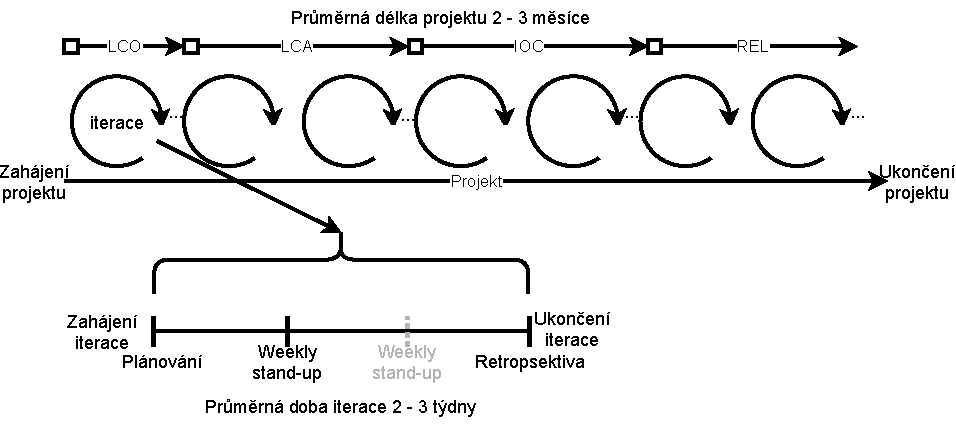
\includegraphics[width=400pt]{img/aswi_proces.pdf}
    \caption{Schéma průběhu ASWI procesu}
    \label{img:aswi_proces}
\end{figure}
\FloatBarrier
\section{Nastavení prahových hodnot}
Některé prahové hodnoty lze nastavit na konkrétní hodnotu, jelikož nejsou závislé na vlastnostech jednotlivých projektů. Avšak většina prahových hodnot je určena výrazem, jehož výsledek určí prahovou hodnotu pro každý projekt individuálně, na základě jeho pozorovaných vlastností. Nastavení prahových hodnot bude probíhat na základě charakteru ASWI procesu popsaného v sekci \ref{sec:aswi_proces}.
\subsubsection{Business As Usual}
\begin{itemize}
    \item X – minimální počet iterací s retrospektivou = \textit{2/3 * počet iterací}
\end{itemize}
Každý projekt může mít jiný počet iterací, je nutné, aby byl minimální počet iterací s retrospektivou závislý na celkovém počtu. Prahová hodnota udávající minimální počet iterací s retrospektivou je vypočtena pomocí vztahu výše. Tato prahová hodnota vyžaduje retrospektivu alespoň u 66,6\% iterací.
\subsubsection{Long Or Non-Existant Feedback Loops}
\begin{itemize}
    \item \texttt{Y1} -- minimální počet iterací, kde se konala alespoň jedna schůzka se zákazníkem = \textit{1/2 * počet iterací}
\end{itemize}

\begin{itemize}
    \item \texttt{Y2} -- maximální rozestup schůzek se zákazníkem (počet dní) = \textit{2 * průměrná délka iterace}
\end{itemize}
V ideálním případě by měla schůzka se zákazníkem probíhat každou iteraci. V některých případech však může dojít k odložení schůzky z důvodu malého posunu v implementaci projektu nebo z časového, proto byla zvolena maximální hodnota rozestupu jako dvojnásobek průměrné délky iterace projektu.
\subsubsection{Ninety-Ninety Rule}
TODO
\subsubsection{Road To Nowhere}
\begin{itemize}
    \item \texttt{I1} -- minimální počet wiki stránek obsahující projektový plán = \textit{1}
\end{itemize}
Většina dostupných projektů vede projektový plán ve wiki stránkách pouze na jedné stránce, je tedy postačující nalézt pouze jednu wiki stránku s projektovým plánem.
\begin{itemize}
    \item \texttt{I2} -- minimální počet aktivit obsahující projektový plán = \textit{1}
\end{itemize}
Projektový plán může vzniknout na základě jedné aktivit, je tedy postačující nalézt pouze jednu aktivitu s projektovým plánem.
\subsubsection{Specify Nothing}
\begin{itemize}
    \item \texttt{J1} -- minimální počet wiki stránek představující specifikaci daného projektu = \textit{1}
    \end{itemize}
V případě vedení specifikace projektu ve wiki stránkách je vedena pouze na jedné stránce. Proto je postačující nalézt jednu wiki stránku představující specifikaci.
    \begin{itemize}
    \item \texttt{J2} -- minimální počet aktivit představující tvorbu specifikace daného projektu = \textit{1}
    \end{itemize}
Specifikaci projektu většinou vytváří samotný projektový tým a následně konzultuje se zadavatelem. Je tedy možné, že bude specifikace vytvářena/upravována vícekrát. Může však dojít k tomu, že je specifikace vytvořena podle představ zákazníka ihned na poprvé. Proto je postačující nalézt alespoň jednu aktivitu, která zmiňuje vytvoření specifikace projektu.  
    \begin{itemize}
    \item \texttt{J3} -- minimální průměrná délka popisku aktivity (počet znaků) = \textit{150}
\end{itemize}
Aby představoval popisek aktivity nějakou vypovídající hodnotu o daném úkolu musí mít alespoň délku 150 znaků. Tato hodnota byla zvolena na základě analýzy délek popisků jednotlivých aktivit, které jsou uloženy ve SPADe.
\subsubsection{Too Long Sprint}
\begin{itemize}
    \item \texttt{K1} -- maximální délka iterace = \textit{21 dní}.
\end{itemize}
V agilní komunitě neexistuje shoda ohledně ideální délky iterace. Metoda Scrum navrhuje délku iterace 3–4 týdny, zatímco Extrémní programování navrhuje délku iterace na 1–2 týdny. \cite{sprint_length} Délka iterace je závislá nejen na dané procesu vývoje softwaru, ale také na velikosti, délce nebo složitosti projektu. Na základě projektů v rámci ASWI procesu, který trvá v průměru 2 - 3 měsíce zvolíme maximální délku iterace na 3 týdny (21 dní). Pokud by byly v rámci těchto projektů nastaveny délky iterací na 4 týdny, došlo by v některých případech pouze ke dvěma iteracím, což je pro velice málo.
\begin{itemize}
    \item \texttt{K2} -- maximální počet příliš dlouhých iterací = \textit{0}.
\end{itemize}
Dle charakteru anti-vzoru Too long sprint byla zvole hodnota této prahové hodnoty na nulu. Jakmile bude jedna iterace (vyjma první a poslední) delší než prahová hodnota, je anti-vzor detekován.
\subsubsection{Varying Sprint Length}
\begin{itemize}
    \item \texttt{L1} -- maximální rozdíl délek dvou po sobě jdoucích iteracích = \textit{7 dní}
\end{itemize}
Pro detekci rozdílných délek iterací je nutné počítat například s výkyvy v řádech jednotek dnů (státní svátek apod.), které mohou ovlivnit délku iterace. Proto byla zvolena jako signifikantní změna délky iterace jeden týden.
\begin{itemize}
    \item \texttt{L2} -- maximální počet signifikantních změn délek iterace. 
\end{itemize}
V rámci projektu je přirozené občas i žádané měnit délku iterace, jelikož prvotní délka iterace nebyla vhodně zvolena. Z tohoto důvodu byla pro detekci odebrána první iterace. Dále byla odebrána poslední iterace, kde může docházet ke zkrácení či prodloužení iterace z důvodu termínu odevzdání projektu. Po odebrání těchto iterací zůstaly iterace z prostředku projektu, kde by měla být délka relativně stálá. Prahová hodnot tedy byla zvolena na hodnotu dvě.
\section{Výsledky}
Úspěšnost implementovaného systému pro detekci anti-vzorů bude vypočtena následujícím vztahem číslo \ref{math:senzitivita}.
\begin{center}
    \label{math:senzitivita}
    \caption{Senzitivita:}
    \begin{equation}
        P(A^{+}|H^{+}) = \frac{a}{a+c}
    \end{equation}
\end{center}
\begin{center}
    \label{math:specificita}
    \caption{Specificita:}
    \begin{equation}
        P(A^{-}|H^{-}) = \frac{d}{b+d}
    \end{equation}
\end{center}
\begin{center}
    \label{math:prediktivní_pozitivní}
    \caption{Prediktivní hodnota pozitivního testu:}
    \begin{equation}
        P(A^{-}|H^{-}) = \frac{d}{b+d}
    \end{equation}
\end{center}
\begin{center}
    \label{math:prediktivní_negativní}
    \caption{Prediktivní hodnota negativního testu:}
    \begin{equation}
        P(A^{-}|H^{-}) = \frac{d}{b+d}
    \end{equation}
\end{center}
Procenta
Výsledky automatické detekce implementovaných anti-vzorů je zobrazen na obrázku č. Výsledky 
\begin{landscape}
\begin{table}[]
\caption{\label{tab:table_result} Výsledky detekce anti-vzorů pomocí realizovaného nástroje}
\begin{tabular}{|l||c|c|c|c|c|c|c|c|c|}
\hline
Anti-vzor& Proj. 1 & Proj. 2 & Proj. 3 & Proj. 4 & Proj. 5 & Proj. 6 & Proj. 7 & Proj. 8 & Proj. 9 \\ \hline \hline
Business As Usual&\xmark&\xmark&\cmark&\xmark&\xmark&\xmark&\cmark&\xmark&\xmark\\ \hline
Long Or Non-Existant Feedback Loops&\cmark&\xmark&\cmark&\cmark&\xmark&\xmark&\xmark&\xmark&\xmark\\ \hline
Ninety-Ninety Rule&TODO&&&&&&&&\\ \hline
Road To Nowhere&\xmark&\xmark&\xmark&\xmark&\xmark&\xmark&\xmark&\xmark&\xmark\\ \hline
Specify Nothing&\cmark&\xmark&\xmark&\cmark&\xmark&\xmark&\xmark&\xmark&\xmark\\ \hline
Too Long Sprint&\cmark&\xmark&\cmark&\xmark&\xmark&\xmark&\xmark&\cmark&\cmark\\ \hline
Varying Sprint Length&\xmark&\xmark&\xmark&\xmark&\xmark&\xmark&\xmark&\cmark&\xmark\\ \hline
\end{tabular}
\end{table}
\textbf{Legenda:}
\begin{itemize}
    \item \cmark -- anti-vzor detekován
    \item \xmark -- anti-vzor nedetekován
\end{itemize}
\FloatBarrier
\newpage
\begin{table}[]
\caption{\label{tab:table_result} Výsledky detekce anti-vzorů pomocí realizovaného nástroje}
\begin{tabular}{|l||c|c|c|c|c|c|c|c|c|}
\hline
Anti-vzor& Proj. 1 & Proj. 2 & Proj. 3 & Proj. 4 & Proj. 5 & Proj. 6 & Proj. 7 & Proj. 8 & Proj. 9 \\ \hline \hline
Business As Usual&\xmark&\xmark&\cmark&\xmark&\xmark&\xmark&\cmark&\xmark&\xmark\\ \hline
Long Or Non-Existant Feedback Loops&\cmark&\xmark&\cmark&\cmark&\xmark&\xmark&\xmark&\xmark&\xmark\\ \hline
Ninety-Ninety Rule&TODO&&&&&&&&\\ \hline
Road To Nowhere&\xmark&\xmark&\xmark&\xmark&\xmark&\xmark&\xmark&\xmark&\xmark\\ \hline
Specify Nothing&\cmark&\xmark&\xmark&\cmark&\xmark&\xmark&\xmark&\xmark&\xmark\\ \hline
Too Long Sprint&\cmark&\xmark&\cmark&\xmark&\xmark&\xmark&\xmark&\cmark&\cmark\\ \hline
Varying Sprint Length&\xmark&\xmark&\xmark&\xmark&\xmark&\xmark&\xmark&\cmark&\xmark\\ \hline
\end{tabular}
\end{table}
\textbf{Legenda:}
\begin{itemize}
    \item \cmark -- anti-vzor detekován
    \item \xmark -- anti-vzor nedetekován
\end{itemize}
\FloatBarrier
\end{landscape}
\section{Diskuze}
TODO
\section{Možná rozšíření}
TODO
\chapter{Závěr}
TODO
 
\bibliographystyle{csplainnatkiv}
{\raggedright\small
\bibliography{literatura}
}
\addcontentsline{toc}{chapter}{Seznam zkratek}
\chapter*{Seznam zkratek}
\begin{itemize}
    \item \textbf{ALM} -- Application Lifecycle Management -- jedná se o nástroje, které jsou využívány k podpoře vývoji softwaru;
    \item \textbf{API} -- Application Programming Interface -- rozhraní pro programování aplikací;
    \item \textbf{CI/CD} -- Continuous Integration/Continuous Deployment -- představuje nástroje a postupy pro správné dodání nové verze softwaru;
    \item \textbf{CVS} -- Concurrent Version System -- systém sloužící ke správě verzí projektu;
    \item \textbf{DMS} -- Document management system -- systém určený ke správě elektronických dokumentů;
    \item \textbf{ETL} -- Extract, transform, load -- proces extrakce, transformace a nahrání dat z jednoho či více zdrojů do datového skladu;
    \item \textbf{JDBC} -- Java Database Connectivity -- rozhraní pro přístup k relačním databázím pomocí jazyka Java;
    \item \textbf{JSON} -- JavaScript Object Notation -- působ zápisu dat nezávislý na počítačové platformě, určený pro přenos dat;
    \item \textbf{J2EE} -- Java 2 Enterprise Edition -- nástroj součástí platformy Java určený pro vývoj a provoz podnikových aplikací a informačních systémů;
    \item \textbf{MVC} -- Model, view, controller -- softwarová architektura, která rozděluje datový model aplikace, uživatelské rozhraní a řídicí logiku do tří nezávislých komponent;
    \item \textbf{PMBOK} -- Project Management Body of Knowledge -- mezinárodně uznávaný standard řízení projektů;
    \item \textbf{PRINCE2} -- Projects in Controlled Environments 2nd version --  flexibilní metodika pro řízení projektů
    \item \textbf{REST} -- Representational state transfer -- architektura rozhraní navržená pro distribuované systémy;
    \item \textbf{SQL} -- Structured Query Language -- standardizovaný strukturovaný dotazovací jazyk, který je používán pro práci s daty v relačních databázích;
    \item \textbf{RUP} -- Rational Unified Process -- metodiky vývoje softwaru pro rozsáhlejší projekty a větší vývojové týmy;
    \item \textbf{XML} -- Extensible Markup Language -- obecný značkovací jazyk, který se používá pro přenos a serializaci dat;
\end{itemize}
\addcontentsline{toc}{chapter}{Seznam obrázků}
\listoffigures
\addcontentsline{toc}{chapter}{Seznam tabulek}
\listoftables
\appendix 
\chapter{Obsah CD}
Popis adresářové struktury a obsahu přiloženého CD:
\begin{itemize}
    \item \texttt{readme.txt} -- Textový soubor popisující obsah cd a adresářovou strukturu.
    \item\texttt{text} -- Složka obsahující text diplomové práce a zdrojové kódy textu
v \LaTeX u.
    \item \texttt{zdrojove\_kody} -- Složka obsahující zdrojové kódy aplikace.
    \item \texttt{Poster} -- Adresář obsahující výsledný poster ve formátu \texttt{pdf} a \texttt{pub.}
\end{itemize}
Základní adresářová struktura je zobrazena na obrázku číslo \ref{img:cd_content}.
\begin{figure}[!htb]
    \centering
    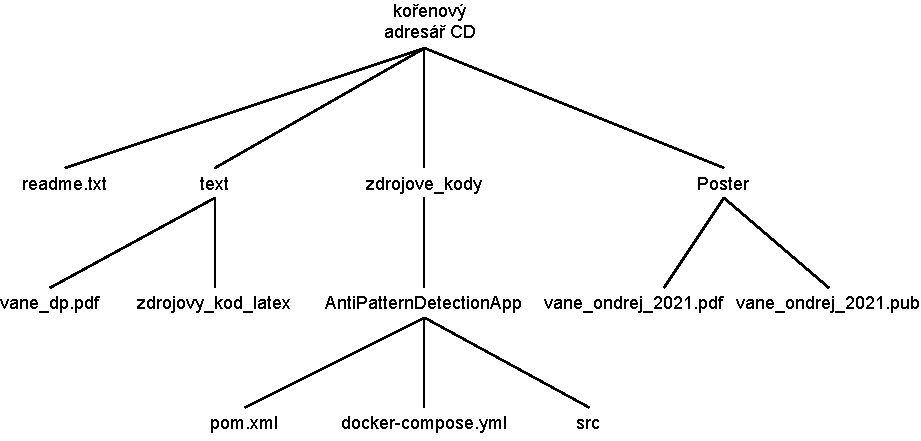
\includegraphics[width=400pt]{img/cd_content.pdf}
    \caption{Adresářová struktura přiloženého CD}    
    \label{img:cd_content}
\end{figure}
\FloatBarrier
\chapter{Příručka nasazení}
Pro usnadnění nasazení aplikace je celkový projekt nakonfigurován pro spuštění v Dockeru. V této příručce je popsáno jak, pomocí nástroje Docker, spustit tuto aplikaci.
\section{Potřebné nástroje}
Ke spuštění aplikace jsou zapotřebí následující nástroje:
\begin{itemize}
    \item Docker \footnote{Příručku pro instalaci nástroje Docker naleznete na adrese \url{https://docs.docker.com/get-docker/}}
    \item Docker Compose \footnote{Příručku pro instalaci nástroje Docker Compose naleznete na adrese \url{https://docs.docker.com/compose/install/}}
    \item GIT \footnote{Příručku pro instalaci nástroje GIT naleznete na adrese \url{https://git-scm.com/book/en/v2/Getting-Started-Installing-Git}} (pouze v případě absence přiloženého CD)
\end{itemize}
\section{Postup spuštění aplikace}
Postup jednotlivých kroků ke spuštění aplikace je popsán v následujícím seznamu: 
\begin{enumerate}
    \item Zkopírovat obsah složky \texttt{AntiPatternDetectionApp} z přiloženého CD nebo pomocí nástroje GIT udělat klon veřejně dostupného repozitáře pomocí následujícího příkazu.
    \newline
    \newline
    \verb|git clone https://github.com/OndrejVane/AntiPatternDetectionApp.git|
    
    \item Otevřít příkazový řádek a přesunout se do kořenové složky projektu s názvem \texttt{AntiPatternDetectionApp}. V této složce by se měl nacházet soubor \texttt{docker-compose.yml}.
    \item V této složce spustit následující příkaz.
    \begin{center}
    \verb|docker-compose build|    
    \end{center}
    Tento příkaz vytvoří potřebné komponenty aplikace, které se v terminologii Dockeru nazývají jako tzv. image.
    \item Po vytvoření potřebných komponent aplikace spustit následující příkaz. \begin{center}
    \verb|docker-compose up -d|    
    \end{center}
    Tento příkaz spustí aplikaci na portu \texttt{8080}. Dále také spustí MySQL databázi na portu \texttt{3306} a rozhraní phpMyAdmin pro administraci databáze na portu \texttt{8082}. Pro správnou funkčnost aplikace je ještě zapotřebí obnovit databázi ze zálohy a databázi nakonfigurovat. Pro obnovení databáze ze zálohy pokračujte do sekce s \ref{section:db_restore} s názvem obnova databáze ze zálohy a konfigurace
\end{enumerate}
\section{Obnova a konfigurace databáze}\label{section:db_restore}
V této části jsou popsány dva postupy pro nastavení a obnovení databáze ze zálohy.
\subsection{Pomocí phpMyAdmin}
\begin{enumerate}
    \item Otevřít rozhraní phpMyAdmin, které běží na portu \texttt{8082}.
    \item Přihlásit se do rozhraní phpMyAdmin pomocí následujících údajů.
    \begin{center}
    Jméno: \verb|root|
    a
    Heslo: \verb|testtest|
    \end{center}
    \item Vytvořit novou databázi s názvem \texttt{spade} a kódováním \texttt{utf8\_unicode\_ci} viz obrázek číslo \ref{img:deploy_php_1}.
    
\begin{figure}[!htb]
    \centering
    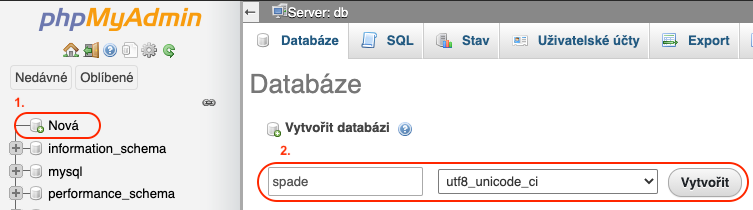
\includegraphics[width=400pt]{img/deploy_php_1.png}
    \caption{Vytvoření databáze}    
    \label{img:deploy_php_1}
\end{figure}
\FloatBarrier
\item Otevřít vytvořenou databázi a přejít do sekce \textit{Import}. Na této obrazovce stisknout tlačítko \textit{Vybrat soubor}. Soubor se zálohou databáze je uložen v kořenové složce projektu s názvem \texttt{db\_dump.sql}. Po vybrání souboru se zálohou stisknout tlačítko \textit{Proveď} v pravém dolním rohu. Postup je znázorněn na obrázku číslo \ref{img:deploy_php_2}. Tím dojde k vytvoření všech potřebných tabulek a pohledů. Pozor tato akce může trvat i několik minut.
\begin{figure}[!htb]
    \centering
    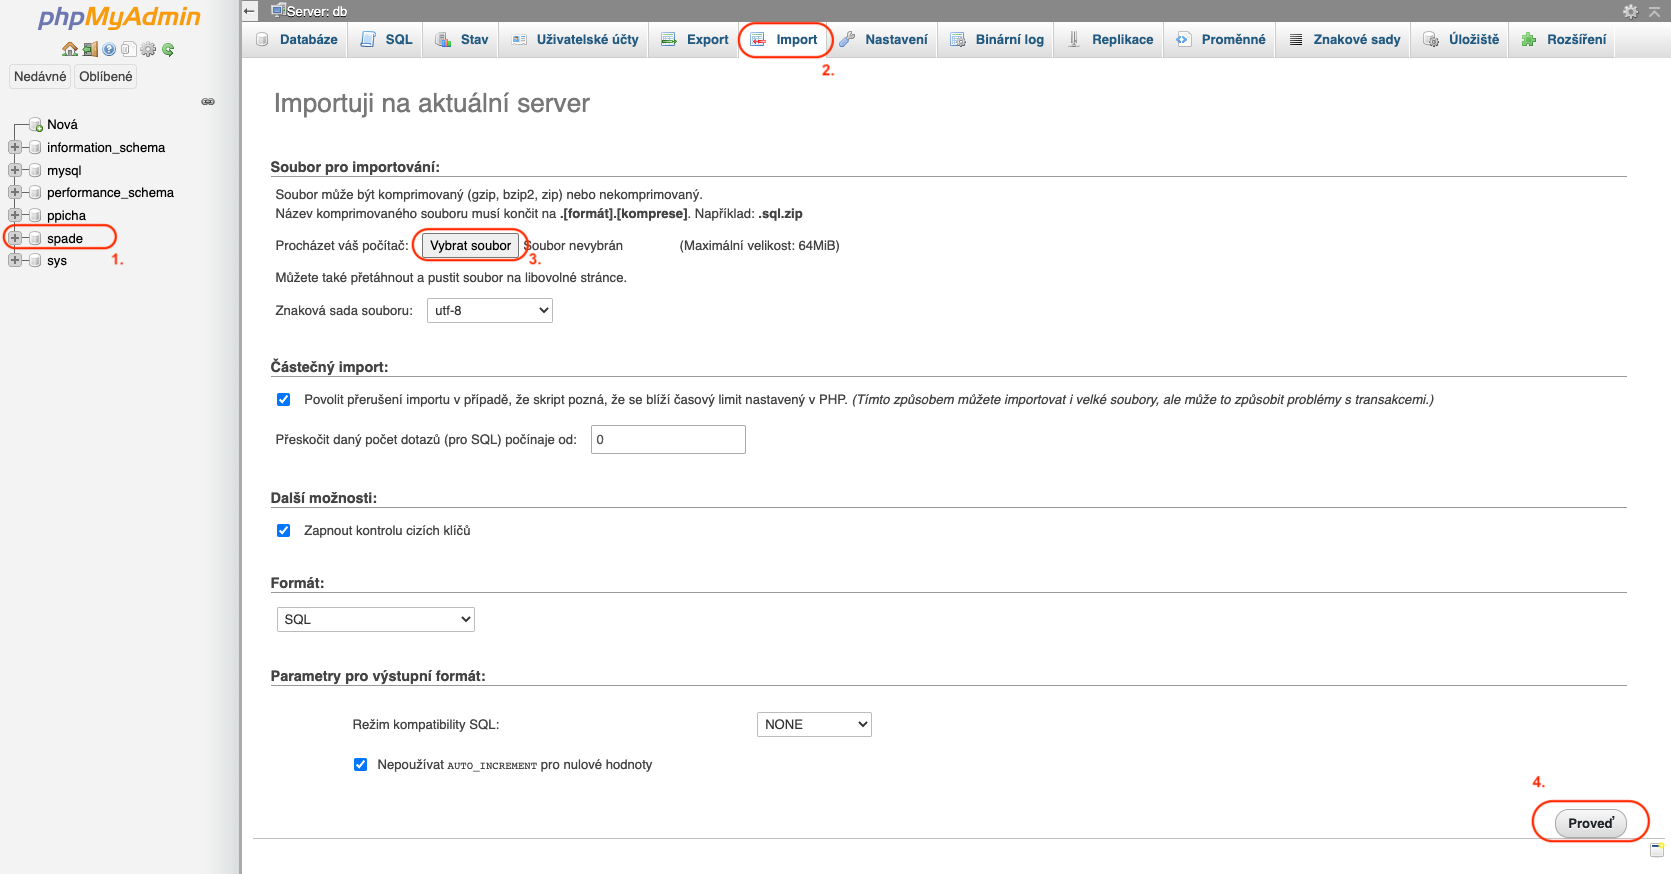
\includegraphics[width=400pt]{img/deploy_php_2.png}
    \caption{Obnova databáze ze zálohy}    
    \label{img:deploy_php_2}
\end{figure}
\FloatBarrier
\item Posledním krokem je konfigurace vytvořené databáze. Pro konfiguraci databáze je zapotřebí obsah souboru \texttt{config.sql}, který je opět uložen v kořenové složce projektu. V phpMyAdmin přejdeme do záložky \textit{SQL}, vložíme obsah souboru do pole pro SQL a stiskneme tlačítko \textit{Proveď} viz obrázek číslo \ref{img:deploy_php_3}. Tím by měla být databáze úspěšně nakonfigurována a aplikace plně funkční.
\begin{figure}[!htb]
    \centering
    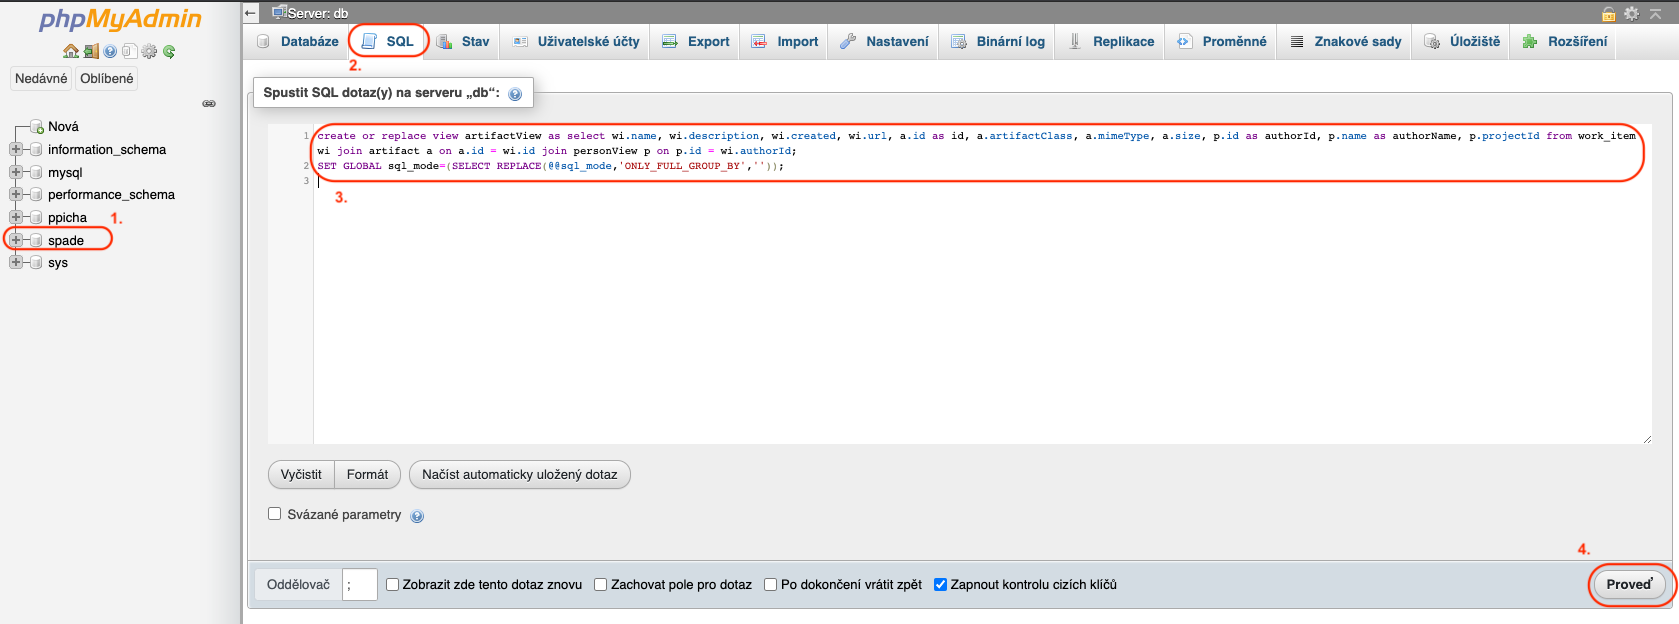
\includegraphics[width=400pt]{img/deploy_php_3.png}
    \caption{Dodatečná konfigurace databáze}    
    \label{img:deploy_php_3}
\end{figure}
\FloatBarrier
\end{enumerate}
\subsection{Pomocí příkazového řádku}
\begin{enumerate}
    \item Spustit v příkazovém řádku následující příkaz.
    \begin{center}
    \verb|docker exec -it mysql-db bin/bash|    
    \end{center}
    Tím dojde k přípojení terminálu k běžícímu kontejneru MySQL databáze.
    \item Přihlásit se do konzole databáze následujícím příkazem.
    \begin{center}
    \verb|mysql -u root -p|    
    \end{center}
    Následně je uživatel vyzván pro vložení hesla pro uživatele \textit{root}.
    \begin{center}
    Heslo: \verb|testtest|    
    \end{center}
    \item V příkazovém řádku MySQL vytvoříme databázi následujícím příkazem.
    \begin{center}
    \verb|create database spade;|    
    \end{center}
    \item Přepnout se do vytvořené databáze následujícím příkazem.
    \begin{center}
    \verb|use spade;|    
    \end{center}
    \item Dále je zapotřebí načíst databázi ze zálohy. Soubor se zálohou je již nakopírován na databázovém serveru. Stačí tedy spustit následující příkaz.
     \begin{center}
    \verb|source /usr/local/etc/db_dump.sql|
    \end{center}
    Tím dojde ke kompletnímu obnově všech tabulek a pohledů. Pozor tato operace může trvat několik minut.
    \item Posledním krokem je konfigurace databáze. Soubor pro konfiguraci je opět nakopírován na databázový server. Stačí spustit následující příkaz.
    \begin{center}
    \verb|source /usr/local/etc/config.sql|
    \end{center}
    Tím dojde ke konfiguraci databází a po tomto kroku by měla být aplikace plně funkční.
\end{enumerate}

\section{Konfigurace aplikace}
Konfigurace celkové aplikace lze provádět v souboru \texttt{docker-compose.yml}. V tomto souboru je možné nakonfigurovat, na kterých portech budou služby spuštěny a také heslo pro připojení do databáze. Pro aplikování změn je nutné restartovat aplikaci. Aktuální soubor je zobrazen níže.
\newline
\begin{lstlisting}
version: '3.3'

services:
  #service 1: definition of mysql database
  db:
    image: mysql:latest
    container_name: mysql-db
    environment:
      - MYSQL_ROOT_PASSWORD=testtest
    ports:
      - "3306:3306"
    restart: always
    volumes:
      - ./db_dump.sql:/usr/local/etc/db_dump.sql
      - ./config.sql:/usr/local/etc/config.sql

  #service 2: definition of phpMyAdmin
  phpmyadmin:
    image: phpmyadmin/phpmyadmin:latest
    container_name: my-php-myadmin
    ports:
      - "8082:80"
    restart: always
    depends_on:
      - db
    environment:
      SPRING_DATASOURCE_USERNAME: root
      SPRING_DATASOURCE_PASSWORD: testtest
    volumes:
      - ./uploads.ini:/usr/local/etc/php/conf.d/uploads.ini

  #service 3: definition of your spring-boot app
  antipatterndetection:
    image: anti-pattern-detection
    container_name: anti-pattern-detection-app
    build:
      context: .
      dockerfile: Dockerfile
    ports:
      - "8080:8080"                 
    restart: always
    depends_on:
      - db
    environment:
      SPRING_DATASOURCE_URL: jdbc:mysql://mysql-db:3306/spade
      SPRING_DATASOURCE_USERNAME: root
      SPRING_DATASOURCE_PASSWORD: testtest

\end{lstlisting}
\subsection{Změna portu}
Port je vždy uváděn v formátu \texttt{<veřejný port>:<port uvnitř kontejneru>}. Pro změnu portu stačí přepsat pouze část nalevo od dvojtečky, tedy veřejný port. Pokud dojde ke změně veřejného portu MySQL databáze, je nutné provést úpravu i na řádku 45, kde je definován JDBC konektor pro aplikaci.
\subsection{Změna hesla databáze}
Heslo pro uživatele \texttt{root} je definováno na řádce číslo devět s označením \texttt{MYSQL\_ROOT\_PASSWORD}. Pokud dojde ke změně tohoto hesla, je nutné ho upravit také na dalších příslušných místech. Konkrétně se jedná o řádky 29 a 47 s označením \texttt{SPRING\_DATASOURCE\_PASSWORD}.
\chapter{Uživatelská příručka}
Aplikace je určena pro přehledné a rychlé analyzování jednotlivých projektů a anti-vzorů.
\section{Detekce anti-vzorů}
Postup detekce anti-vzorů je popsán v následujícím seznamu.
\begin{enumerate}
    \item Otevřít prohlížeč a přejít na hlavní stránku aplikace. V horní části obrazovky se nachází hlavní navigační menu, v levé části se nachází tabulka s projekty a v pravé části tabulka s anti-vzory. Hlavní obrazovka je zobrazena na obrázku číslo \ref{img:user_screen_1}.
\begin{figure}[!htb]
    \centering
    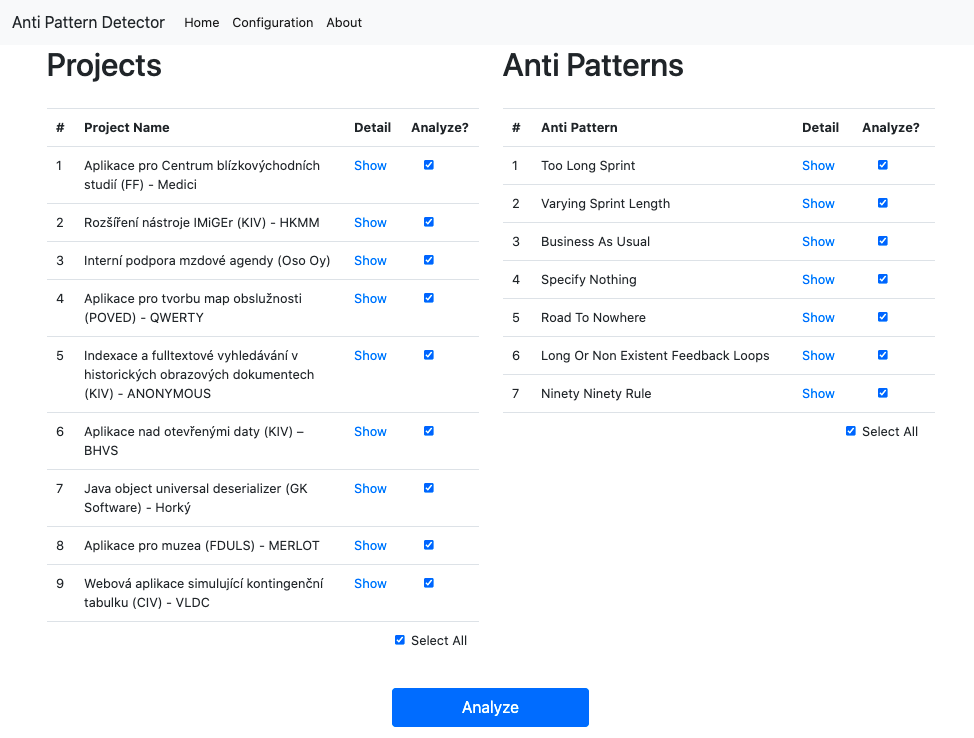
\includegraphics[width=350pt]{img/user_screen_1.png}
    \caption{Hlavní obrazovka aplikace}    
    \label{img:user_screen_1}
\end{figure}
\FloatBarrier
    \item Vybrat všechny projekty, které chcete analyzovat. Pozor musí být vybrán alespoň jeden projekt (v případě nevybrání žádného projektu se zobrazí hláška viz obrázek číslo \ref{img:user_screen_2b}). Pro výběr daného projektu použijte zaškrtávací políčko viz obrázek číslo \ref{img:user_screen_2}. Pro označení nebo odznačení všech projektů použijte zaškrtávací políčko \texttt{Select All}.
\begin{figure}[!htb]
    \centering
    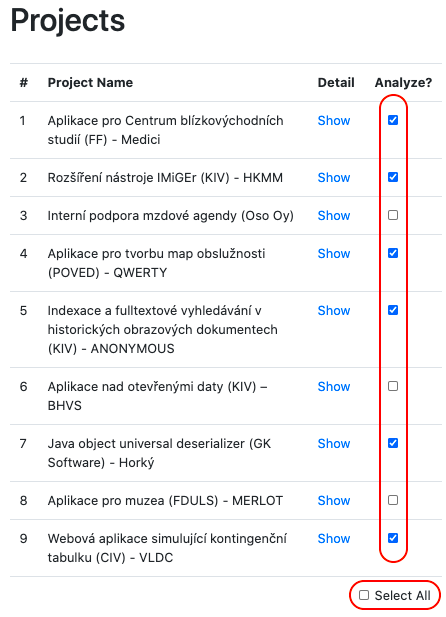
\includegraphics[width=200pt]{img/user_screen_2.png}
    \caption{Výběr projektů}    
    \label{img:user_screen_2}
\end{figure}
\begin{figure}[!htb]
    \centering
    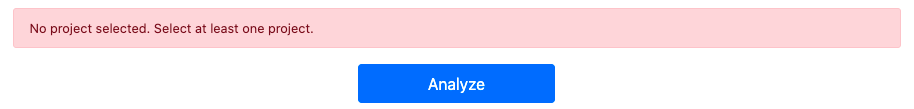
\includegraphics[width=400pt]{img/user_screen_2b.png}
    \caption{Chybová hláška -- žádný vybraný projekt}    
    \label{img:user_screen_2b}
\end{figure}
\FloatBarrier
    \item Vybrat všechny anti-vzory, které chcete ve vybraných projektech detekovat. Pozor musí být vybrán alespoň jeden anti-vzor (v případě nevybrání žádného anti-vzoru se zobrazí hláška viz obrázek číslo \ref{img:user_screen_3b}). Pro výběr daného anti-vzoru použijte zaškrtávací políčko viz obrázek číslo \ref{img:user_screen_3}. Pro označení nebo odznačení všech anti-vzorů použijte zaškrtávací políčko \texttt{Select All}.
\begin{figure}[!htb]
    \centering
    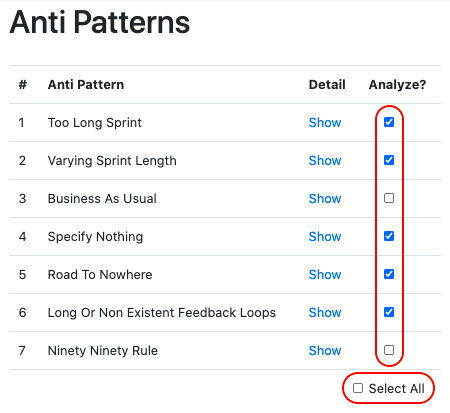
\includegraphics[width=200pt]{img/user_screen_3.png}
    \caption{Výběr anti-vzorů}    
    \label{img:user_screen_3}
\end{figure}
\begin{figure}[!htb]
    \centering
    
\includegraphics[width=400pt]{img/user_screen_3b.png}
    \caption{Chybová hláška -- žádný vybraný anti-vzor}    
    \label{img:user_screen_3b}
\end{figure}
\FloatBarrier
    \item Po vybrání příslušných projektů a anti-vzorů stačí stisknout tlačítko \texttt{Analyze}.
    \item Po dokončení analýzy dojde k zobrazení tabulky s výsledky detekce a legendy viz obrázek číslo \ref{img:user_screen_4}.
\begin{figure}[!htb]
    \centering
    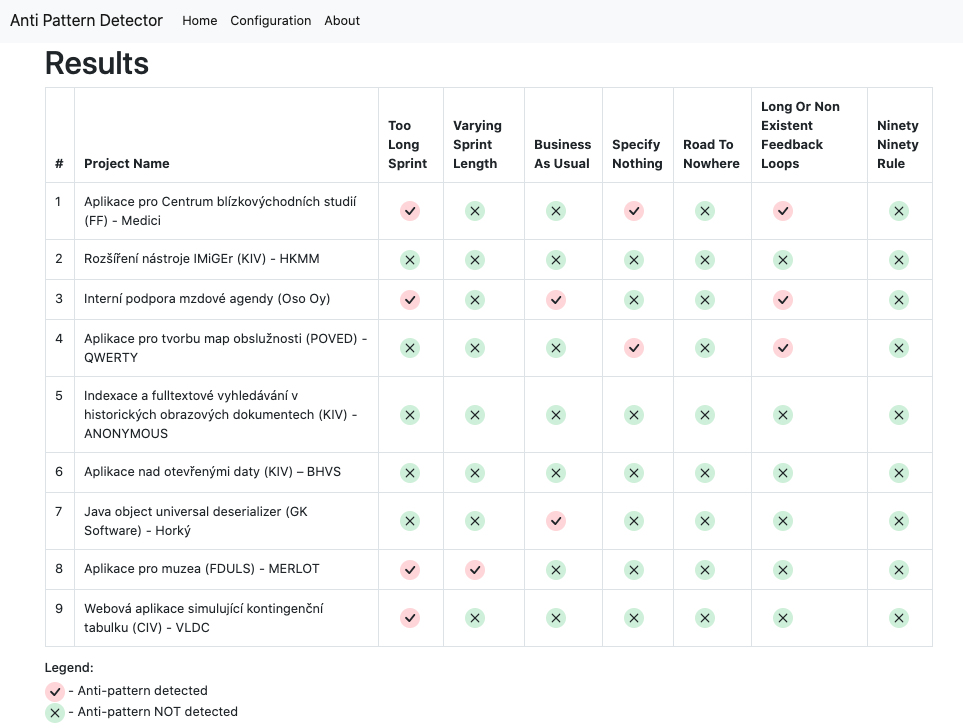
\includegraphics[width=350pt]{img/user_screen_4.png}
    \caption{Výsledná tabulka}    
    \label{img:user_screen_4}
\end{figure}
\FloatBarrier
    \item U každého výsledku detekce lze zobrazit dialogové okno s podrobnostmi o detekci. Dialogové okno lze zobrazit po kliknutí na ikonu, která znázorňuje výsledek detekce anti-vzoru u příslušného projektu viz obrázek číslo \ref{img:user_screen_10}.
\begin{figure}[!htb]
    \centering
    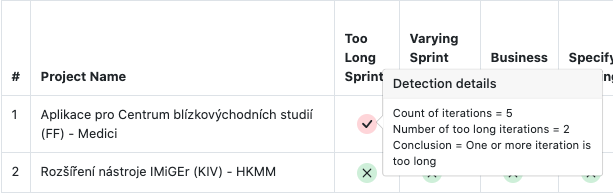
\includegraphics[width=350pt]{img/user_screen_10.png}
    \caption{Zobrazení podrobností o detekci}    
    \label{img:user_screen_10}
\end{figure}
\FloatBarrier
    \item Pro opětovný výběr projektů nebo anti-vzorů stiskněte tlačítko \texttt{Back Home} nebo tlačítko \texttt{Home} v hlavním menu viz obrázek číslo \ref{img:user_screen_5}. Tím dojde k otevření hlavní stránky aplikace.
\begin{figure}[!htb]
    \centering
    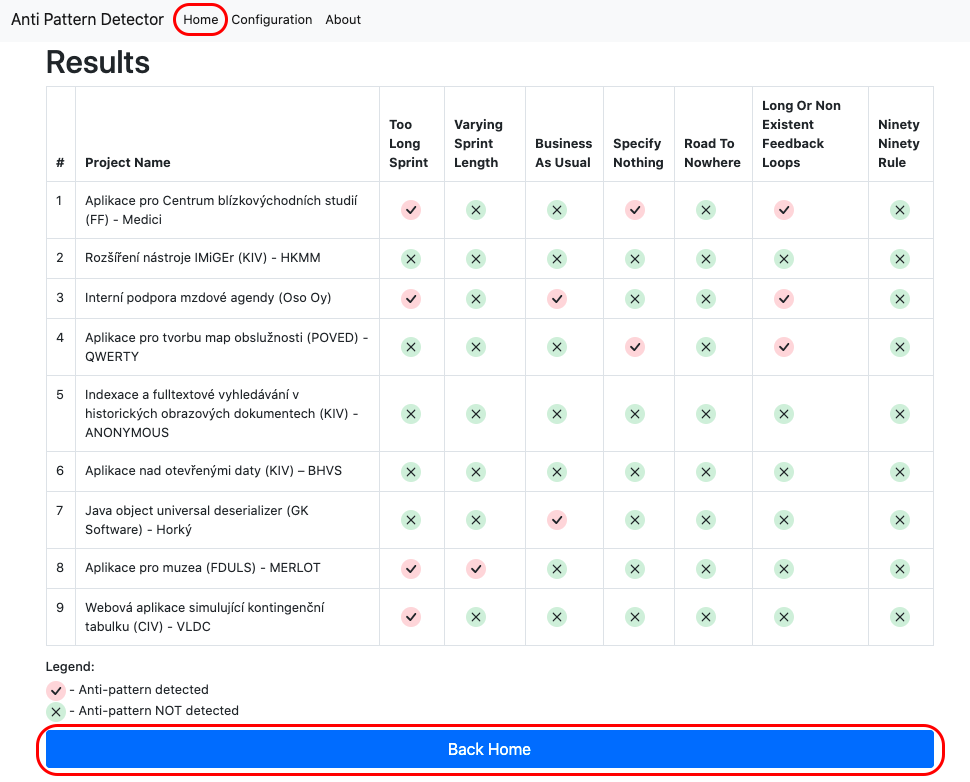
\includegraphics[width=350pt]{img/user_screen_5.png}
    \caption{Návrat na hlavní stránku}
    \label{img:user_screen_5}
\end{figure}
\FloatBarrier
\end{enumerate}
\section{Konfigurace prahových hodnot}
Pomocí výsledné aplikace lze konfigurovat jednotlivé prahové hodnoty, které byly definovány v kapitole číslo \ref{sec:antipattern_analyzation}. Postup pro nastavení prahových hodnot je popsán v následujícím seznamu.
\begin{enumerate}
    \item Přejít na stránku konfigurace pomocí tlačítka \texttt{Configuration} v hlavním menu viz obrázek číslo \ref{img:user_screen_11}.
    \begin{figure}[!htb]
    \centering
    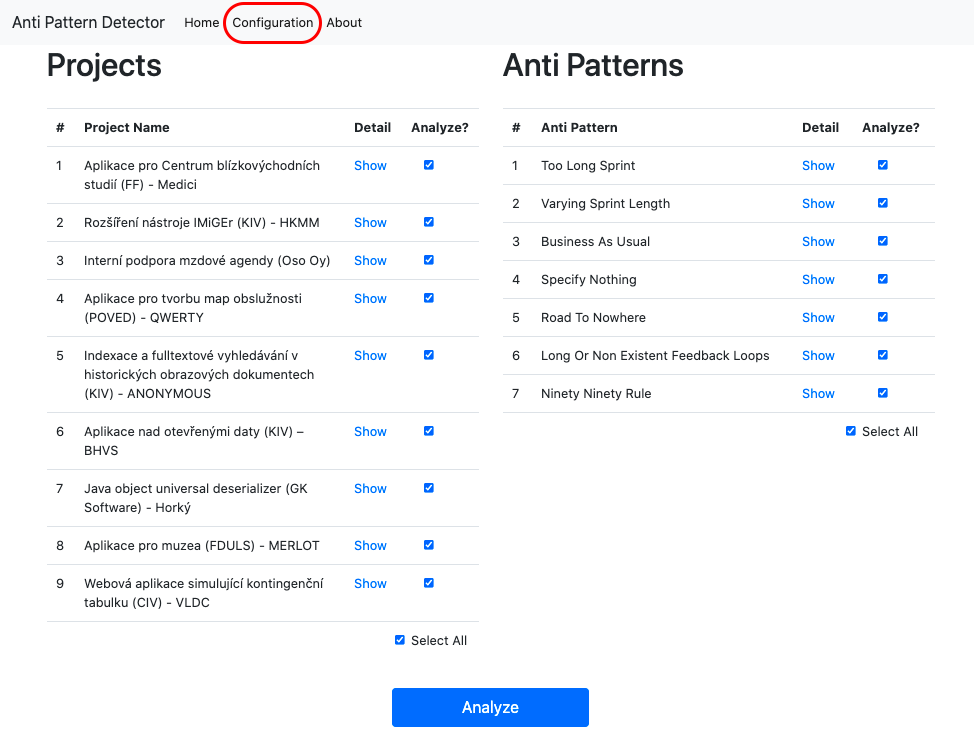
\includegraphics[width=350pt]{img/user_screen_11.png}
    \caption{Zobrazení seznamu prahových hodnot}
    \label{img:user_screen_11}
\end{figure}
\FloatBarrier
    \item Následně se zobrazí seznam všech implementovaných anti-vzorů a jejich aktuálně nastavených prahových hodnot viz obrázek číslo \ref{img:user_screen_22}.
    \begin{figure}[!htb]
    \centering
    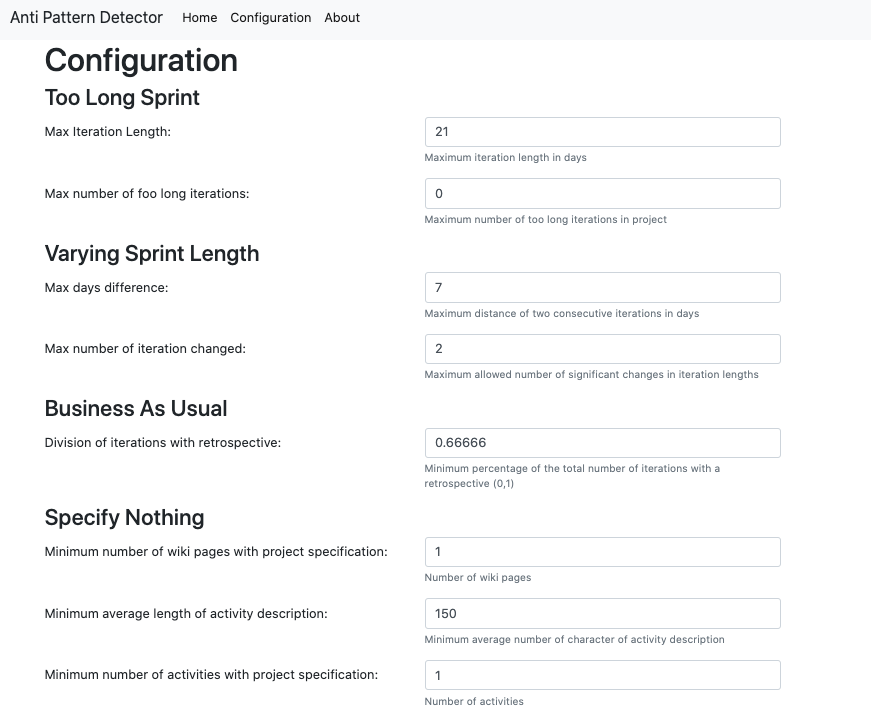
\includegraphics[width=350pt]{img/user_screen_22.png}
    \caption{Zobrazení prahových hodnot}
    \label{img:user_screen_22}
\end{figure}
\FloatBarrier
    \item Pro editaci jedné nebo více prahových hodnot stačí přepsat číselnou hodnotu u dané prahové hodnoty a následně stisknout tlačítko \texttt{Save} ve spodní části obrazovky viz obrázek číslo \ref{img:user_screen_33}.
    \begin{figure}[!htb]
    \centering
    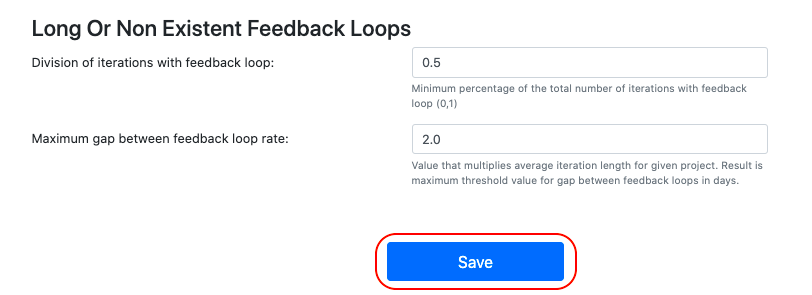
\includegraphics[width=350pt]{img/user_screen_33.png}
    \caption{Uložení prahových hodnot}
    \label{img:user_screen_33}
\end{figure}
\FloatBarrier
    \item V případě, že byly hodnoty správně nastaveny, dojde k zobrazení hlášky viz obrázek číslo \ref{img:user_screen_44}.
    \begin{figure}[!htb]
    \centering
    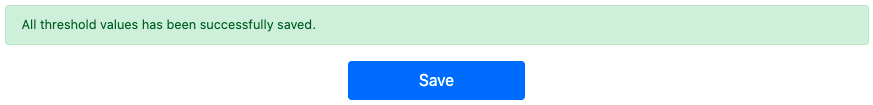
\includegraphics[width=400pt]{img/user_screen_44.png}
    \caption{Hláška o úspěšném uložení prahových hodnot}
    \label{img:user_screen_44}
\end{figure}
\FloatBarrier
    \item V případě neúspěšného uložení dojde k výpisu chybové hlášky viz obrázek číslo \ref{img:user_screen_55} a je nutné nastavení prahových hodnot upravit a zopakovat.
    \begin{figure}[!htb]
    \centering
    
\includegraphics[width=400pt]{img/user_screen_55.png}
    \caption{Hláška o neplatném nastavení prahových hodnot}
    \label{img:user_screen_55}
\end{figure}
\FloatBarrier
\end{enumerate}
\section{Zobrazení informací o projektu}
Aplikace umožňuje zobrazení základních informací o vybraném projektu. Postup pro zobrazení informací o projektu je popsán v následujícím seznamu.
\begin{enumerate}
    \item Přejít na hlavní stránku aplikace.
    \item Stisknout tlačítko \texttt{Show} vedle projektu, u kterého chcete zobrazit podrobnosti viz obrázek číslo \ref{img:user_screen_6}.
\begin{figure}[!htb]
    \centering
    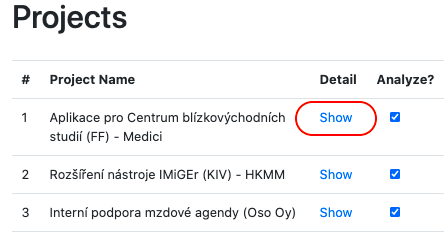
\includegraphics[width=300pt]{img/user_screen_6.png}
    \caption{Zobrazení podrobností o projektu}
    \label{img:user_screen_6}
\end{figure}
\FloatBarrier
    \item Následně se zobrazí obrazovka s informacemi o projektu viz obrázek číslo \ref{img:user_screen_7}.
\begin{figure}[!htb]
    \centering
    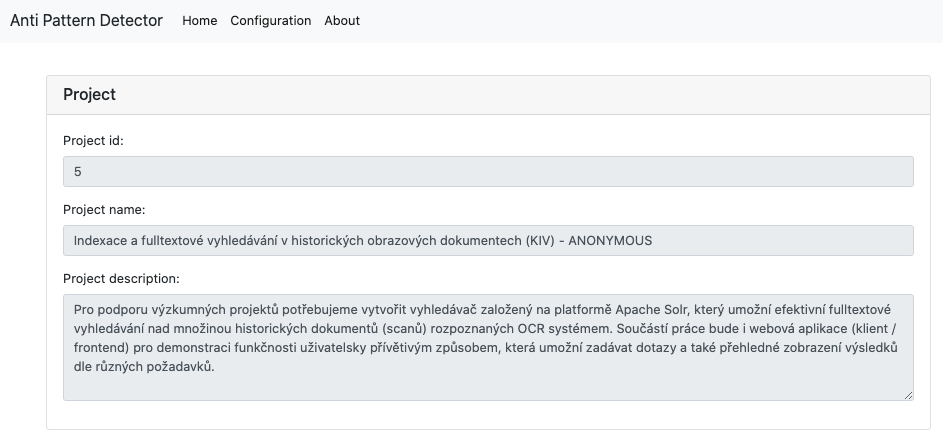
\includegraphics[width=400pt]{img/user_screen_7.png}
    \caption{Podrobnosti o vybraném projektu}    
    \label{img:user_screen_7}
\end{figure}
\FloatBarrier
\end{enumerate}
\section{Zobrazení informací o anti-vzoru}
Aplikace umožňuje zobrazení základních informací o vybraném anti-vzoru. Postup pro zobrazení informací o anti-vzoru je popsán v následujícím seznamu.
\begin{enumerate}
    \item Přejít na hlavní stránku aplikace.
    \item Stisknout tlačítko \texttt{Show} vedle anti-vzoru, u kterého chcete zobrazit podrobnosti viz obrázek číslo \ref{img:user_screen_8}.
\begin{figure}[!htb]
    \centering
    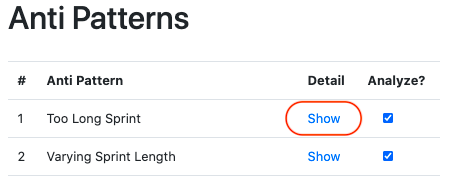
\includegraphics[width=300pt]{img/user_screen_8.png}
    \caption{Zobrazení podrobností o anti-vzoru}
    \label{img:user_screen_8}
\end{figure}
\FloatBarrier
    \item Následně se zobrazí obrazovka s informacemi o anti-vzoru a všechny jeho prahové hodnoty viz obrázek číslo \ref{img:user_screen_9}.
\begin{figure}[!htb]
    \centering
    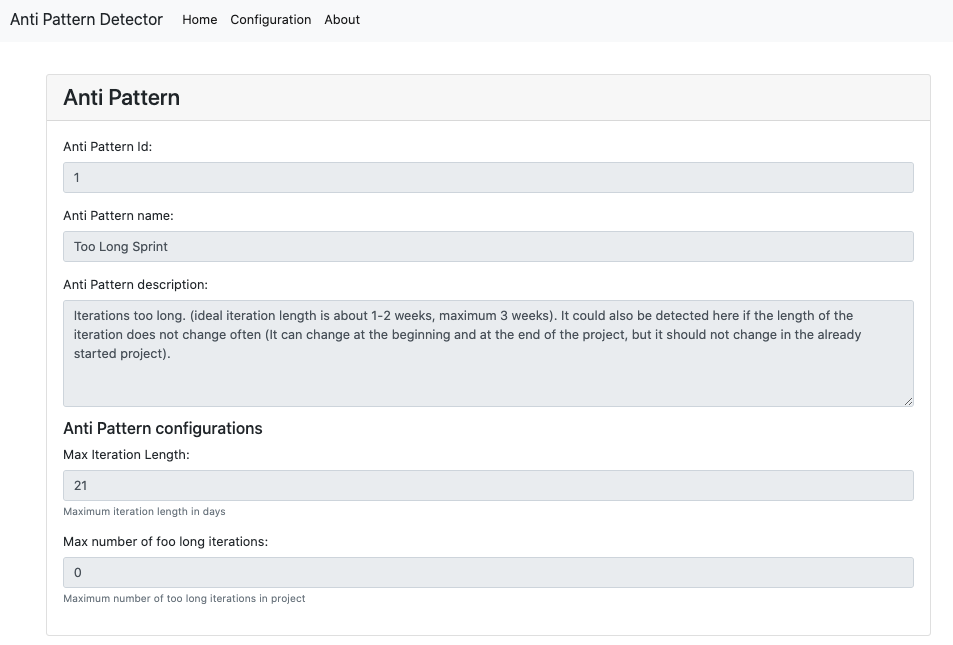
\includegraphics[width=400pt]{img/user_screen_9.png}
    \caption{Podrobnosti o vybraném anti-vzoru}
    \label{img:user_screen_9}
\end{figure}
\FloatBarrier
\end{enumerate}
\end{document}
